%\chapter*[Normative references]{NORMATIVE REFERENCES}

%Following standards used in this work
%Text

% English
\chapter*[Abstract]{ABSTRACT}
% краткая выжимка, включающая описание цели, проделлано работы и полученных результатов
The purpose of this thesis is to research and implement the MLOps methodology while considering cybersecurity principles for software engineering, using on-premises technologies as an alternative to cloud providers or other providers in order to ensure the security of confidential data storage. The theoretical aspects of MLOps investigated in this study supported the development of a more effective process for working with potential stakeholders and applying scientific knowledge of DS in practice. Application development was performed using a variety of modern Python libraries and frameworks, as well as the PostgreSQL relational database. Furthermore, a pre-trained LLM was deployed and monitored utilizing Docker containerization for hosting. The findings are directly applicable in practical contexts for industry-standard practices and future research activities.

% Russian
%\chapter*[Аннотация]{АННОТАЦИЯ}
%Целью данной дипломной работы является исследование и внедрение методологии MLOps, учитывая принципы кибербезопасности при разработке программного обеспечения с использованием on-premises технологий, в качестве альтертативы cloud провайдерам или другим сервисам, для обеспечения безопасности хранения конфиденциальных данных. Изученные теоретические аспекты MLOps способствовали разработке более эффективного процесса работы с потенциальными заинтересованными сторонами и применения научных знаний о DS на практике. Разработка приложения осуществлялась с использованием множества современных библиотек и фреймворков на Python, а также с применением реляционной базы данных PostgreSQL. Кроме того, была развернута предобученная LLM, над которой производился мониторинг с применением средств контейниризации Docker для хостинга. Полученные результаты напрямую применимы в практическом плане для отраслевых методик и будущей исследовательской деятельности.

% Kazakh
%\chapter*[Аңдатпа]{АҢДАТПА}
%Бұл дипломдық жұмыстың мақсаты құпия деректерді сақтау қауіпсіздігін қамтамасыз ету үшін cloud провайдерлерге немесе басқа провайдерлерге балама ретінде on-premises технологияларды пайдалана отырып, бағдарламалық жасақтама жасау үшін киберқауіпсіздік принциптерін қарастыра отырып, MLOps әдіснамасын зерттеу және енгізу болып табылады. Зерттелген MLOps теориялық аспектілері әлеуетті мүдделі тараптармен жұмыс істеу және DS ғылыми білімін тәжірибеде қолдану үшін тиімдірек процесті дамытуға қолдау көрсетті. Қолданбаларды әзірлеу әр түрлі заманауи Python кітапханалары мен фреймворктерін, сондай-ақ PostgreSQL реляциялық деректер базасын пайдалану арқылы орындалды. Сонымен қатар, хостинг үшін Docker контейнеризациясын пайдалану арқылы алдын ала дайындалған LLM орналастырылды және бақыланды. Нәтижелер салалық стандартты тәжірибелер мен болашақ зерттеу әрекеттері үшін практикалық контексттерде тікелей қолданылады.






\chapter*[Definitions]{DEFINITIONS}

Following terms are used in this work:

\begin{definitions}[4cm] % ширина метки терминов (по умолчанию 3 см)
    %-------------------
    \item [DevOps] - a methodology that emerged as a shift paradigm for the tech industry for addressing both social and technical issues via applying processes around the Agile manifesto.
    %-------------------
    \item [MLOps] - a fusion of DevOps and machine learning, represents a collection of concepts for implementing machine learning products in a practical environment, including automation processes within the development and business spheres.
    %-------------------
    \item [Web scraping] - a process of data extraction from various web resources.
    %-------------------
\end{definitions}







\chapter*[Designations and abbreviations]{DESIGNATIONS AND ABBREVIATIONS}

Following designations and abbreviations are used in this work:

\begin{glossaries}[3cm] % ширина метки обозначений (по умолчанию 2 см)
    %-------------------
    \item [IT] Information Technology
    %-------------------
    \item [ML] Machine Learning
    %-------------------
    \item [DL] Deep Learning
    %-------------------
    \item [DS] Data Science
    %-------------------
    \item [Ops] Operations
    %-------------------
    \item [MLOps] Machine Learning Operations
    %------------------- 
    \item [NLP] Natural Language Processing
    %-------------------
    \item [API] Application Programming Interface
    %-------------------
    \item [LLM] Large Language Model
    %-------------------
    \item [AI] Artificial Intelligence
    %-------------------
    \item [PoC] Proof of Concept
    %-------------------
    \item [SOTA] State-of-the-art
    %-------------------
    \item [IDE] Integrated Development Environment 
    %-------------------
    \item [R\&D] Research and Development
    %-------------------
    \item [SaaS] Software as a Service
    %-------------------
    \item [CI] Continuous Integration
    %-------------------
    \item [CD] Continuous Deployment
    %-------------------
    \item [CT] Continuous Training
    %-------------------
    \item [REST] Representation State Transfer
    %-------------------
    \item [RPC] Remote Procedure Call
    %-------------------
    \item [KPI] Key Performance Indicators
    %-------------------
    \item [ROS] Return on Sales
    %-------------------
    \item [ЕTL] Extract Transform Load
    %-------------------
    \item [ЕLT] Extract Load Transform
    %-------------------
\end{glossaries}








\chapter*[Introduction]{INTRODUCTION}

\textbf{Work relevance.} 
% Сфера data science в последнее время очень популярна - поэтому появляется множество исследований и проектов направленных на это, однако они попросту терпят провалы или плохо масштабируемые - поэтому есть MLOps который способствует качественному прогрессу и обеспечивает грамотные подходы и вместе со стандартами безопасности с cybersecurity
From a marketing standpoint, companies are increasingly adopting DS solutions to thrive in the IT industry, driving demand for SaaS platforms. However, these platforms raise concerns about data confidentiality, internal functionality, security features, and the cost-effectiveness of subscriptions. Proprietary solutions from commercial organizations also negatively impact the open-source community by reducing transparency and trust. Additionally, deploying SaaS solutions is more expensive than local applications. Therefore, effective model deployment to production requires MLOps methodologies, which integrate machine learning experts, developers, and system administrators, accelerating processes and ensuring web application security.

\textbf{Research object.} Overall, the research object is the process of creating products that are strategically designed to integrate with various forms of MLOps technologies. This idea is accomplished through identifying possible approaches within its general context of the area.

\textbf{Research subject.} Moreover, the subject of this study focuses on the integration considerations of advanced cybersecurity principles in web services. It also covers a comprehensive assessment of practical issues, such as business operations, implementation phases, along with other interrelated concepts.

\textbf{Goal of the work.} In alignment with the thesis topic, the primary project direction is aimed at developing a complete web application of textual data process automation according to modern industry-standard practices.

\textbf{Objectives:}
\begin{enumerate}
    %----------
    \item Construct an API web service based on technological trends, architectural solutions, and security design methods.
    %----------
    \item Research and implement the MLOps methodology by organizing procedures of development, testing, deployment, hosting pipeline, and ensuring replicable workflow throughout the entire lifecycle of the product.
    %----------
\end{enumerate}

\textbf{Research methodology.} The theoretical methods were primarily established on the information analysis and synthesis of previously identified objectives. Examined research materials encompassed different scientific literature, courses, academic articles and publications, conference proceedings, supplementary sources, etc. Furthermore, the collection of resources was assembled through publicly accessible data on the internet and platforms focused on scholarly material searches, including Google Scholar or Mendeley. Additionally, there was applied a knowledge base technique involving the use of storage for condensed information. On the contrary, practical methods were aligned towards experimental and observational approaches. Therefore, comparative metrics, measurements, and evaluations were conducted by comparing with similar open-source solutions, due to the declaration of a tangible product as a result of the project.

\textbf{Work significance.} The theoretical significance revolves around the concept of summarizing crucial commercial, scientific, and public literature in order to formulate a theoretical foundation or conceptual consensus. Thus, it provides opportunities for readers to comprehend an actual background behind formerly mentioned technological areas and their current state. Consequently, these insights might contribute as a basis element for the creation of a specialized course within the domain of cybersecurity as well as further detailed research. On the other hand, the practical value of the project could be utilized in local enterprises and commercially driven startups, because it addresses business-oriented challenges.

\textbf{Novelty.} The thesis represents a cutting-edge perspective on the topic of MLOps integration using state-of-the-art technologies, revealing novel aspects of the topic. However, this technique remains relatively understudied and demands significant computational power, leading to certain companies monopolizing the integration of LLM for instance. Those who are unable to adapt would become outsiders in the information technology market. Hence, this study stands out by attempting to provide a phased overview of the theme and identifying development standards for domestic products. The emphasis is considered on manageable and cost-effective methods. This means that the practical approach encompasses application protection along with the consistency of storage, confidentiality, integrity, availability, collection, and processing of data as critical resources for language models.

% \textbf{Structure of the work.} 








\chapter[Theoretical part]{THEORETICAL PART}
% тут нужно небольшое предисловие - небольшое объяснение что в этой теоретической части будет раскрыто и для чего это нужно

\section[What is MLOps?]{What is MLOps?}
% MLOps as a part of data science
The general field of data science strives to solve data-driven problems. This means that its entire concept is built around the processing and application of data in the form of complex systems. Commonly, there are many misconceptions about data scientists, one of which is the belief that they must be multifaceted specialists in all areas of data science. Recently, this discipline has been distinctly divided into a combination of different directions, as shown in figure \ref{fig.1.1}: science (scientific competencies and research), domain (domain-specific and business expertise), development (software engineering and programming) \cite{natekin_alexey_2018}. As a result, the proportional distribution of these features shapes dynamic subclasses of data science professions such as ML engineer, data analyst, data engineer, MLOps, analyst, ML researcher, etc.

\begin{figure}[h]
\centering
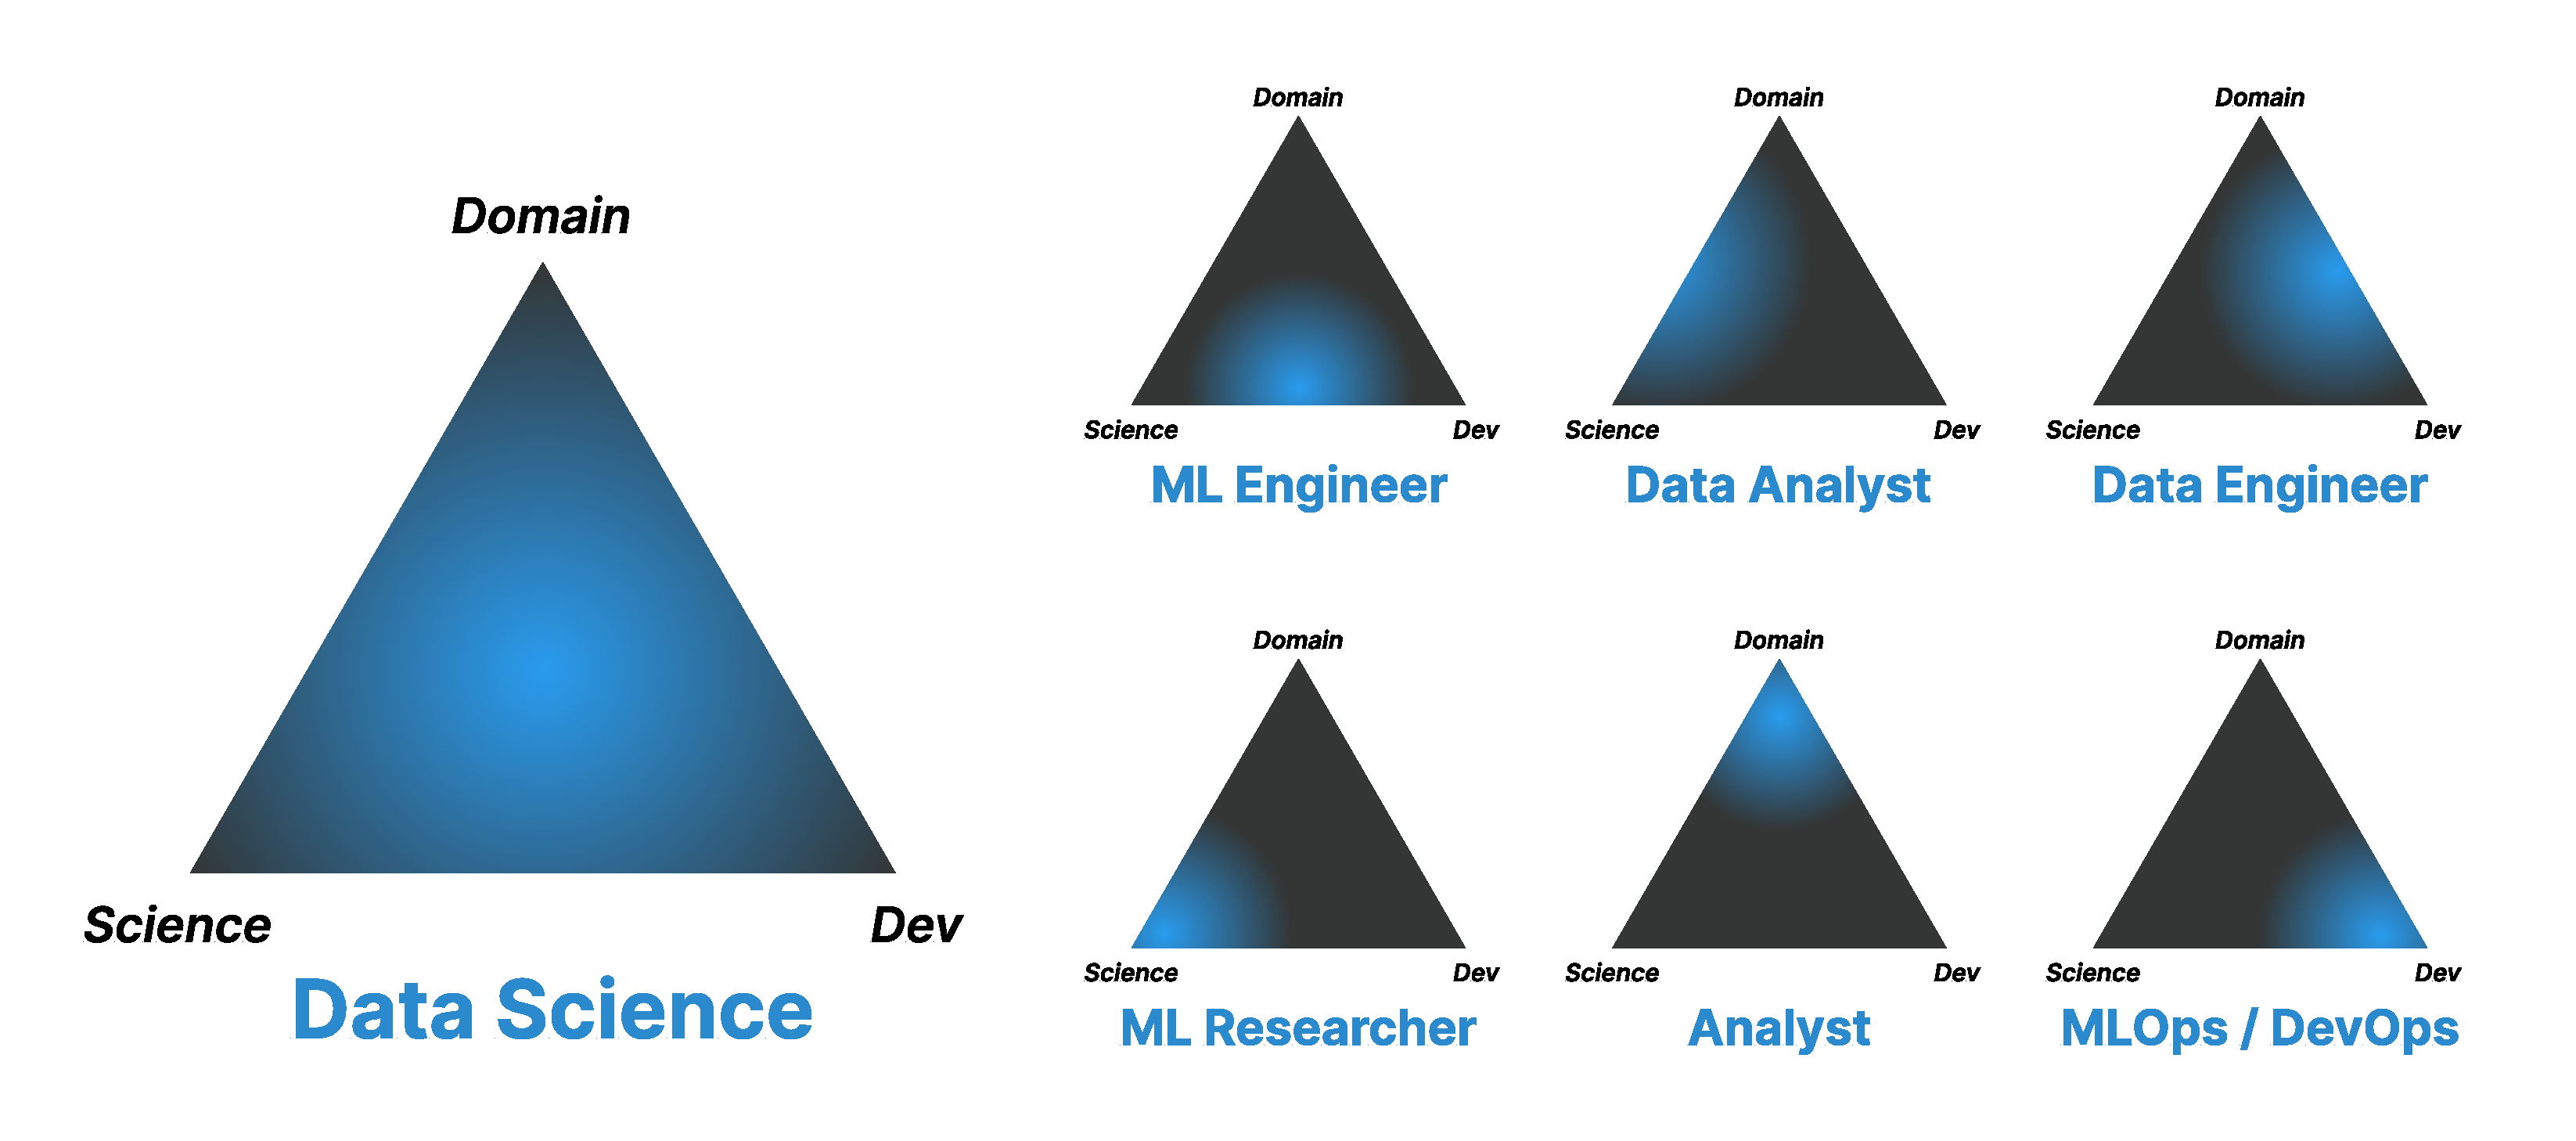
\includegraphics[width=1.0\textwidth]{figures/figure_1_1.pdf}
% \\
% \parbox[t]{\textwidth}{\vspace{1ex}\large\hspace*{7.5mm}Description}
\captionsetup{style=figureStyle}
\caption{Directions and combinations of data science aspects\cite{natekin_alexey_2018}}\label{fig.1.1}
\end{figure}

% About MLOps, MLOps as a part of DevOps, актуальность подхода, связь с другими дисциплинами
Among these emerging specializations, one particularly notable area is MLOps, which is still a vague term. It only started to gain popularity after the rise of DevOps and the strengthening of Ops mindsets. The primary factors for its widespread dissemination have been commercialization through out-of-the-box tools as well as the growing demand for cloud environments \cite{kreuzberger_d_2022}. In this context, cloud providers like Amazon, Google, or Alibaba offer significant advantages through bulk storage and computational VMs to avoid maintenance costs by providing a pay-as-you-go or SaaS subscription model \cite{zhou_y_2020}. That case clearly demonstrates its inherent benefits. Transitioning to the broader perspective, DevOps represents a methodology that emerged as a shift paradigm for the tech industry for addressing both social and technical issues via applying processes around the Agile manifesto \cite{kreuzberger_d_2022}. Unlike traditional approaches, it has significantly enhanced collaboration and interaction within large-scale projects, leading to substantial expertise among professionals in its practices. Broadly speaking, MLOps, as a fusion of DevOps and machine learning, represents a collection of concepts for implementing machine learning products in a practical environment, including automation processes within the development and business spheres. According to Kreuzberger et al., MLOps teams require more than just data scientists; they involve interdisciplinary collaboration including stakeholders, architects, data engineers, software engineers, etc. in order to achieve the true effectiveness and objectives of MLOps \cite{kreuzberger_d_2022}.

To understand the reasons behind the adoption of MLOps methodology by organizations, it is beneficial to examine the research survey conducted by Makinen et al. This survey explores a wide range of Ops-oriented companies in the market, including small teams (11-30 individuals), scale-ups (151-500 employees), and enterprises (1001 and more employees). Authors declare that organizations typically evolve gradually before transitioning to MLOps, so this progression occurs as they address production issues and advance in their ML maturity, moving from a data-centric approach to a model-centric one and eventually expanding to a pipeline-centric model \cite{makinen_s_2021}. Therefore, MLOps is more suitable for experienced teams that understand how to handle various challenges and manage unrealistic expectations effectively.


\section[The replication crisis in MLOps]{The replication crisis in MLOps}
Replication is an essential component of any practically-oriented scientific experiment, which is a procedure for achieving valid results for a methodological part of the study. In general, it shows that outcomes are not random in pre-provisioned circumstances. According to the latest publication standards, the Association for Computing Machinery highlights three forms of that indicator: relatability ('same team, same experimental setup'), reproducibility ('different team, same experimental setup'), and replicability ('different team, different experimental setup') \cite{plesser_h_e_2018}. Despite the fact that it is necessary to strictly follow requirements (i.e., hardware, software, data acquisition, or historical boundaries) in order to implement PoC in data science, a fundamental study published by Nature has already raised the insight that about 60 percent of scientific publications in engineering and technical fields contain false-positive results and difficult-to-reproduce experiments \cite{baker_m_2016}. According to Martinez et al., nearly 90 percent of data science projects never reach production state, indicating that this is a risky venture \cite{martinez_i_2021}. For example, these articles may fail to account for certain metrics, overlook numerous auxiliary factors during measurements, use legacy methodology, and so on. Moreover, technical issues are escalated by the widespread application of Jupyter Notebooks among data scientists. According to a study about public repositories on Github, nearly 65 percent of these notebooks suffer from dependency or environment issues, execution order problems, and the absence of necessary external files \cite{pimentel_j_f_2019}. These challenges are part of anti-patterns that must be addressed to prevent the accumulation of technical debt, as minor errors can destabilize ML systems due to their CACE principle (Changing Anything Changes Everything) \cite{sculley_d_2015}. Therefore, the philosophy of MLOps aims to address and provide comprehensible methodologies for all the aforementioned confusions in production. For example, Breck et al. emphasize the importance of using testing checklists to identify critical oversights like untested code, inadequate evaluation methods, and biases \cite{breck_e_2017}. Additionally, it is in demand to utilize a specialized IDE for running short code scripts, as Jupyter Notebooks are best suited for quick experiments or code snippets rather than primary development artifacts. For instance, these Bash or Python scripts are integral to pipeline automation in end-to-end processes, enabling CI, CD, and CT to automate ML re-training, versioning, and configuration \cite{faubel_l_2023}. Meanwhile, the final model must be packaged in backend containers and accessed through REST or RPC interfaces, using standardized APIs to facilitate system integration \cite{kolltveir_a_b_2022}. Furthermore, any subsequent experiment should be documented during the research process in the form of step-by-step descriptions or a wiki. On the other hand, the code base has to be maintained with comments, proper styling, linters, formatters, templating of structure-based file organization, and dependencies. Overall, production systems are not completely about coding but also involve leveraging collaborative and complex infrastructures, as visualized in figure 1.2.

\begin{figure}[h]
\centering
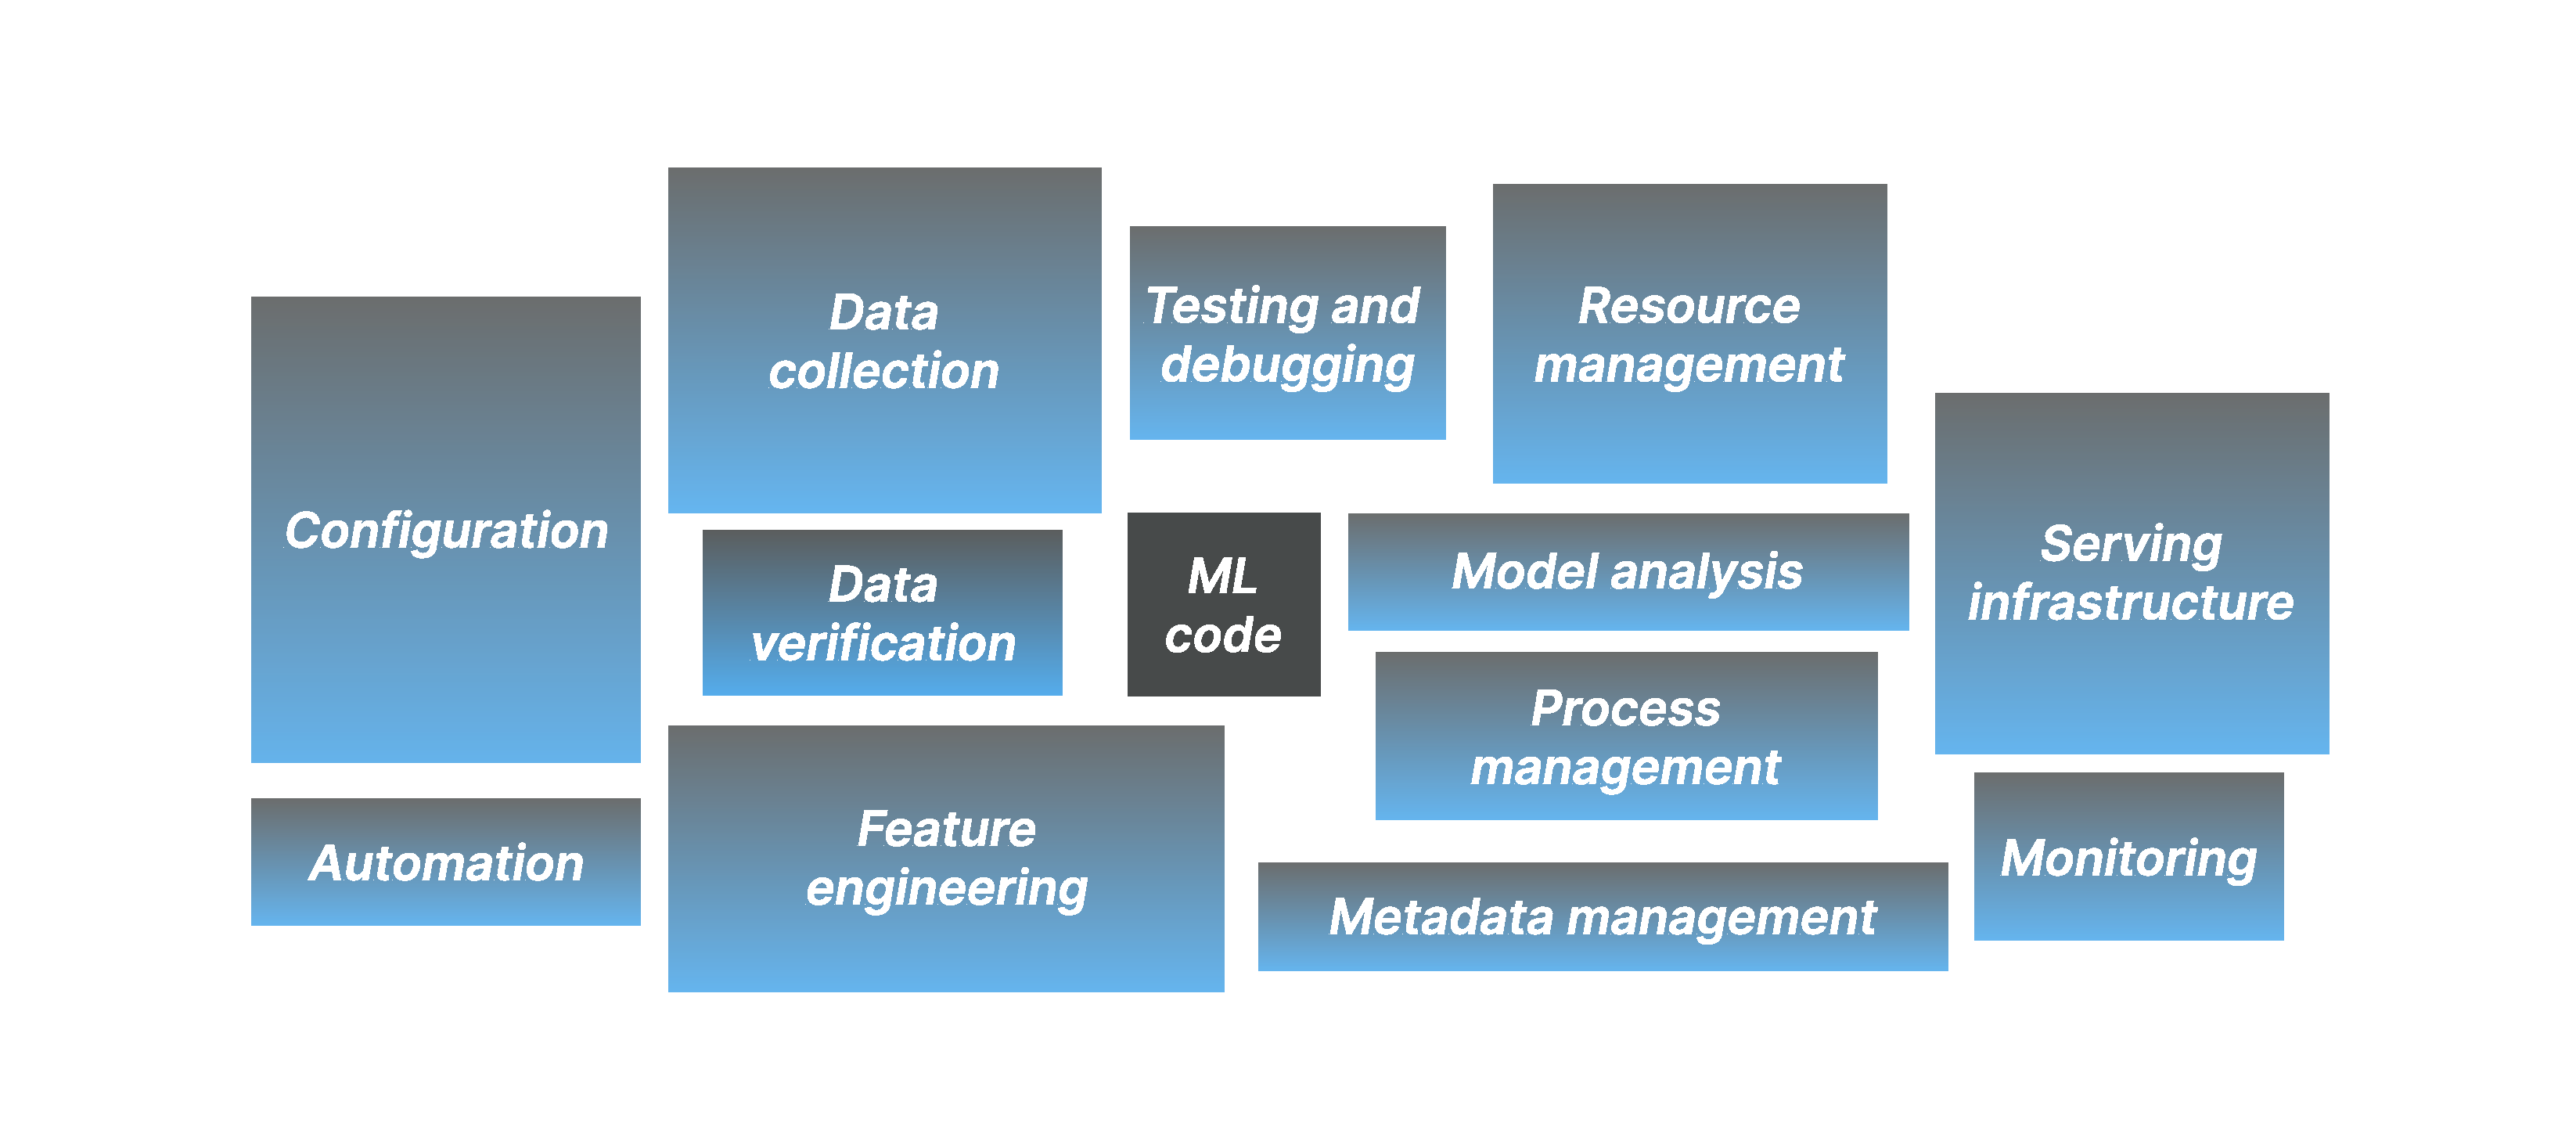
\includegraphics[width=1.0\textwidth]{figures/figure_1_2.pdf}
% \\
% \parbox[t]{\textwidth}{\vspace{1ex}\large\hspace*{7.5mm}Description}
\captionsetup{style=figureStyle}
\caption{Structure of data science projects\cite{sculley_d_2015}}\label{fig.1.2}
\end{figure}


\section[Data in MLOps]{Data in MLOps}
Data plays a significant role as an important resource similar to oil, serving as the foundation of any data science project, particularly in data-centric tasks \cite{pan_i_2022}. Its quality and volume have a direct influence on model performance. Generally, these tasks are commonly referred to data engineering and are required to develop effective procedures and pipelines around data. However, data engineering is often confused as big data which only refers to the scale of data and the corresponding toolkit required. It is commonly defined by 5 V's (volume, velocity, variety, veracity, value) and only represents a subset field within data science that focuses on data distribution and parallel processing \cite{martinez_i_2021}. Technologies such as Hadoop and Apache Spark have transformed data storage and parallel processing, with the escalation in computational power, particularly from GPUs, while the increased scale of data exacerbates technology complexity, infrastructure requirements, and associated costs \cite{munawar_h_s_2022}. For instance, certain articles claim that data engineering consists of several sub-stages \cite{faubel_l_2023, testi_m_2022}:

- Data collection involves multiple stages including data extraction, preparation, and transformation. Firstly, data extraction or gathering can utilize domain-related sources and multiple methods such as web scraping, querying records, and real-time sensors for data acquisition. Secondly, data preparation involves exploratory data analysis to understand data schemas and characteristics expected by the model. Finally, data engineers construct consistent pipelines for preliminary transformations, including cleaning and splitting into train, test, and validation datasets. However, throughout the process, there may arise risks about customer data, such as availability, sufficiency, processing time, and annotation quality \cite{martinez_i_2021}. Therefore, a data assessment is necessary, evaluating processing complexity, sample object counts, domain-related patterns, annotation quality, and the handling of outliers or missing values. Additionally, experts recommend extending the data pool via creating variations of existing data through data augmentation or applying transfer learning \cite{testi_m_2022}.

- Data management serves as a supportive stage, facilitating tasks such as data labeling and versioning. Data labeling tools help data science teams in annotating large datasets, while data versioning tools assist both data science and engineering teams in managing model and dataset versions. These tools enable teams to gain insights into how data changes affect model performance and how datasets evolve over time.

% Объяснение про ETL / ELT (Сбор данных, хранение, обработка)
% Объяснение про Базы данных и хранилища данных (data lakes , data warehouses)
% Объяснение про парсинг и вебскрапперы
The processes described above are also known in some sources as ETL/ELT pipelines. According to Souibgui et al., ETL integration involves aggregating different final results in data warehouses while ensuring high data quality through professional tooling and step-by-step processing via streaming and batching data delivery \cite{souibgui_m_2019}. The main distinction between ETL and ELT lies in the stage at which transformation occurs. In ELT, data transformation is postponed until after loading unprocessed data, a process gaining popularity due to rapidly changing business requirements \cite{mukherjee_r_2017}, as represented in figure 1.3.

\begin{figure}[h]
\centering
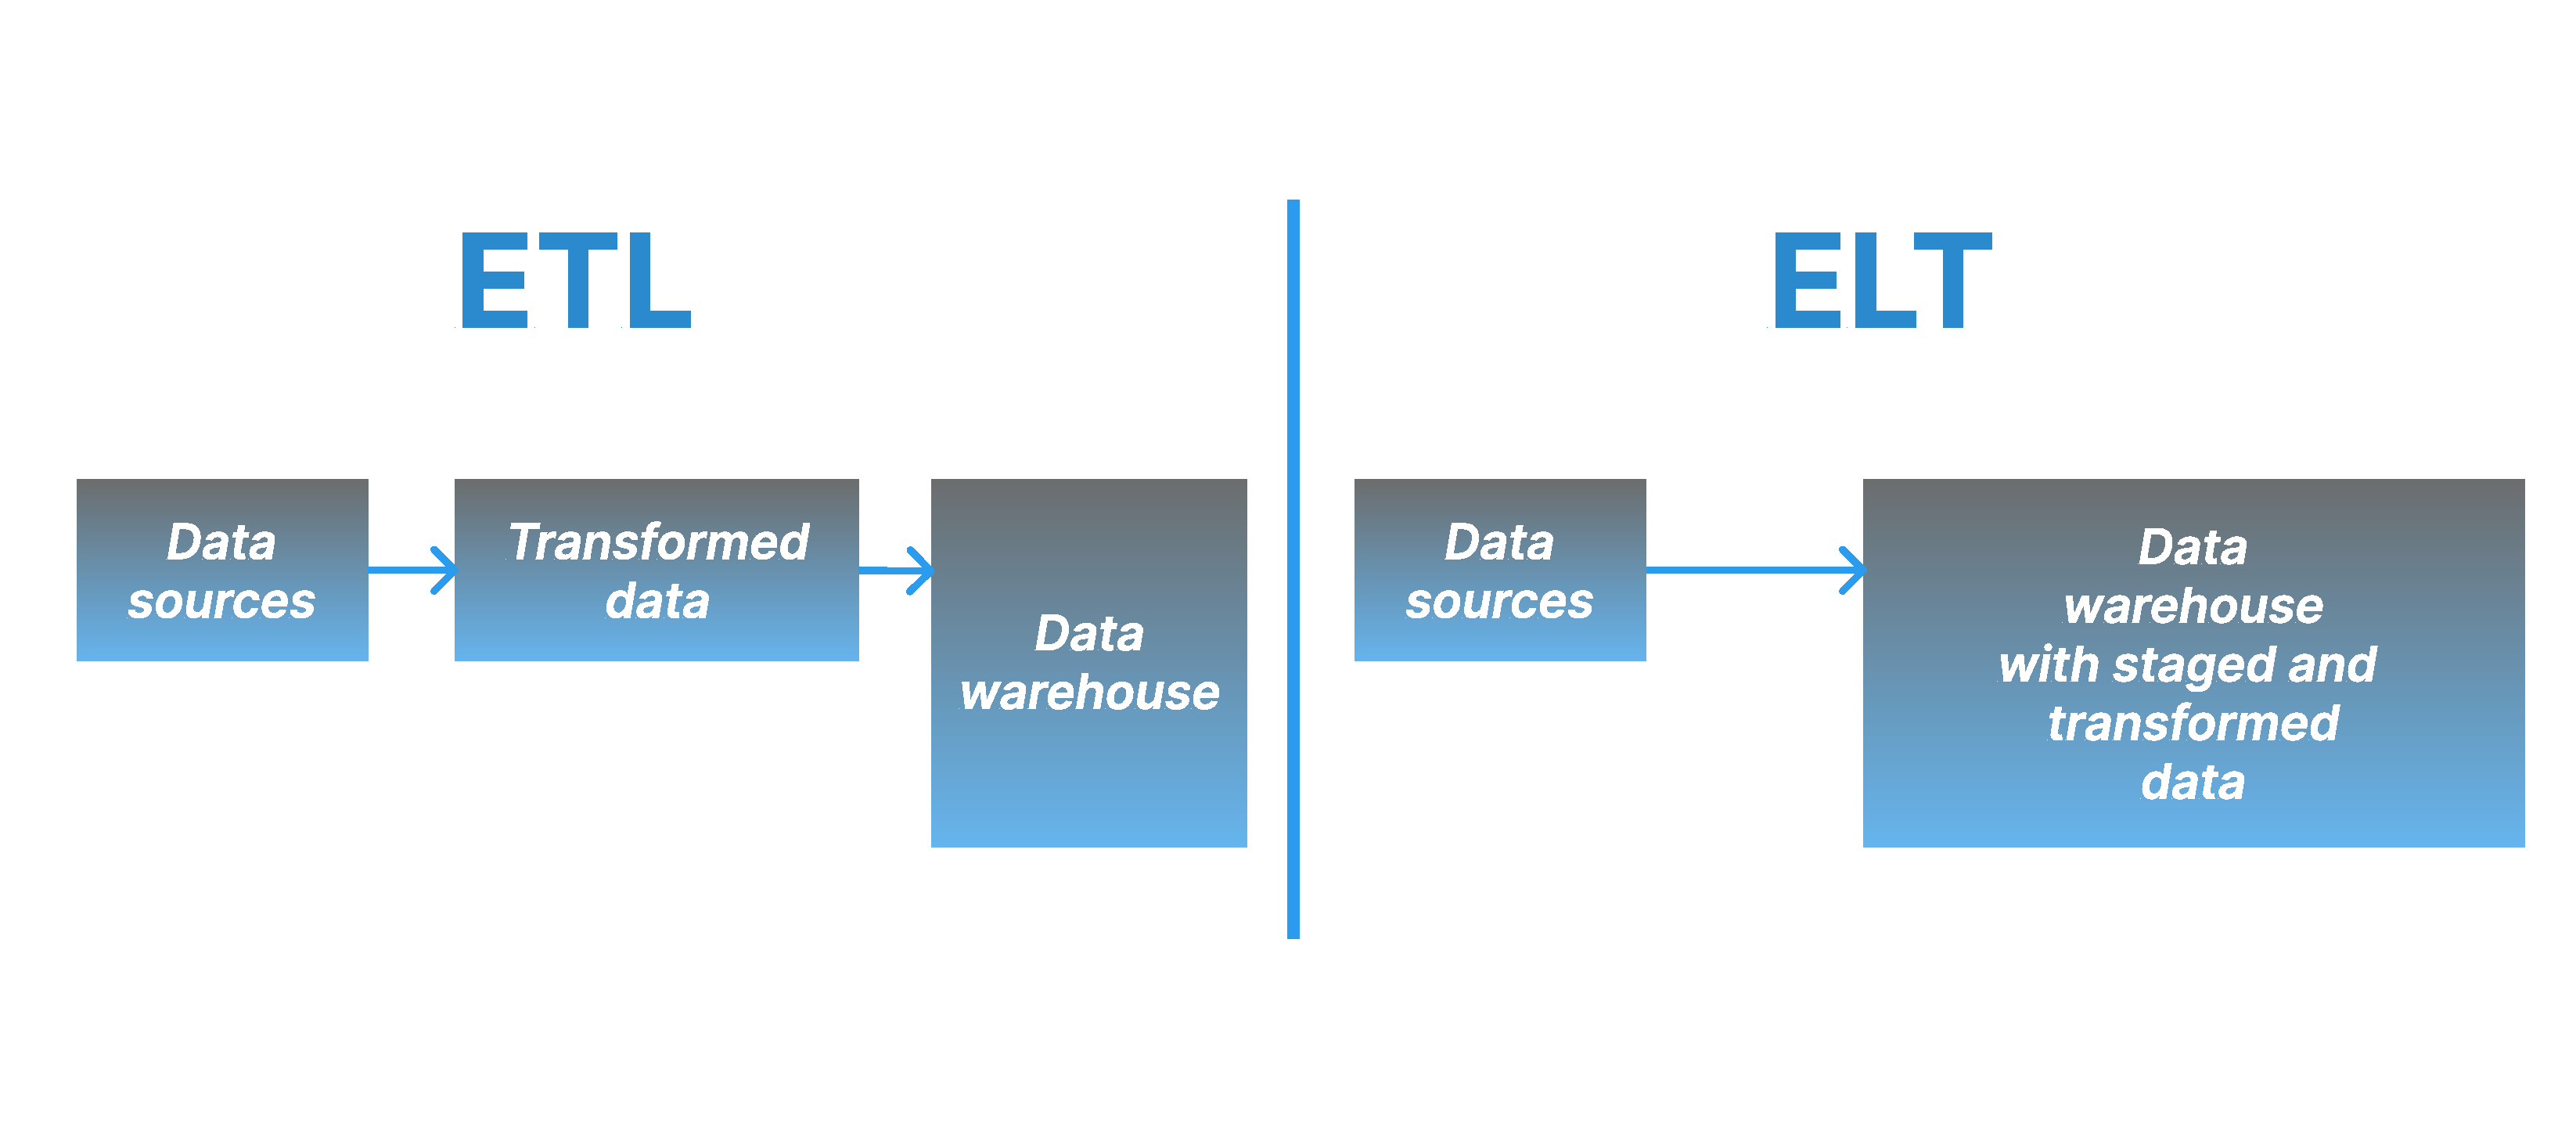
\includegraphics[width=1.0\textwidth]{figures/figure_1_3.pdf}
% \\
% \parbox[t]{\textwidth}{\vspace{1ex}\large\hspace*{7.5mm}Description}
\captionsetup{style=figureStyle}
\caption{ETL/ELT pipelines\cite{mukherjee_r_2017}}\label{fig.1.3}
\end{figure}

% Объяснение про Шифрование и безопасность данных при их хранении, какая связь с ИБ существует
From a cybersecurity standpoint, there are numerous concerns regarding data handling. For instance, data security and privacy management involves safeguarding information from denial-of-service attacks and unauthorized access or modification through authentication, authorization, data anonymization, and access tracking methods. Authentication typically involves usernames and passwords, limiting user data access, while access tracking logs details like dataset requests, data manipulation, and access validity. Data anonymization conceals sensitive data before user presentation, although merged data sources may potentially deanonymize information \cite{davoudian_a_2020}.

% \section[MLOps in NLP domain]{MLOps in NLP domain}
% Немного про мл и дл направления - работа с разными доменами
% Если углубляться в домейны, то их огромная куча: computer vision, natural language, robotics, и т.д. Однако если смотреть по направления специализированным есть мл, дл, рл и другое - они именно специализированные направления, а не домейны
% Architectures and solutions in MLOps
% Углубление в нлп, концепцию поиска данных, популярные архитектуры в нлп, про эмбединги, векторные вычисления и движки, промты, высокоуровнивые подходы и популярные фишки (RAG, Few Shot, etc.)

\section[Workflow and management optimization in MLOps]{Workflow and management optimization in MLOps}
% Про то как MLOps влияет на работу в команде + достижение результатов заказчика в бизнесе
The MLOps workflow seamlessly involves collaboration with both team members and stakeholders. At the initiation phase of any project, step-by-step assessment and analysis of business requirements is a critical phase: evaluation of feasibility, practicality, resource estimation, and formulation of a technical specification. According to the best practices of Kim et al., Ops patterns can be delivered in three forms of business interactions: 'the first way' (optimizing workflow without intervals, so it enhancing visibility and products are safe to change), 'the second way' (establishing rapid and continuous feedback loop throughout to prevent recurring problems), 'the third way' (fostering a culture of proactive improvement of trust and experimentation for multiple feedback loops) \cite{kim_g_2016}. In addition, studies of Faubel et al. support this theory and clearly demonstrate that MLOps is an ongoing cycle of triggers for business tasks and their resolutions, as represented in figure 1.4 \cite{faubel_l_2023}. Fundamentally, this structure views business as having a central role in guiding critical decisions and strategic directions.

\begin{figure}[h]
\centering
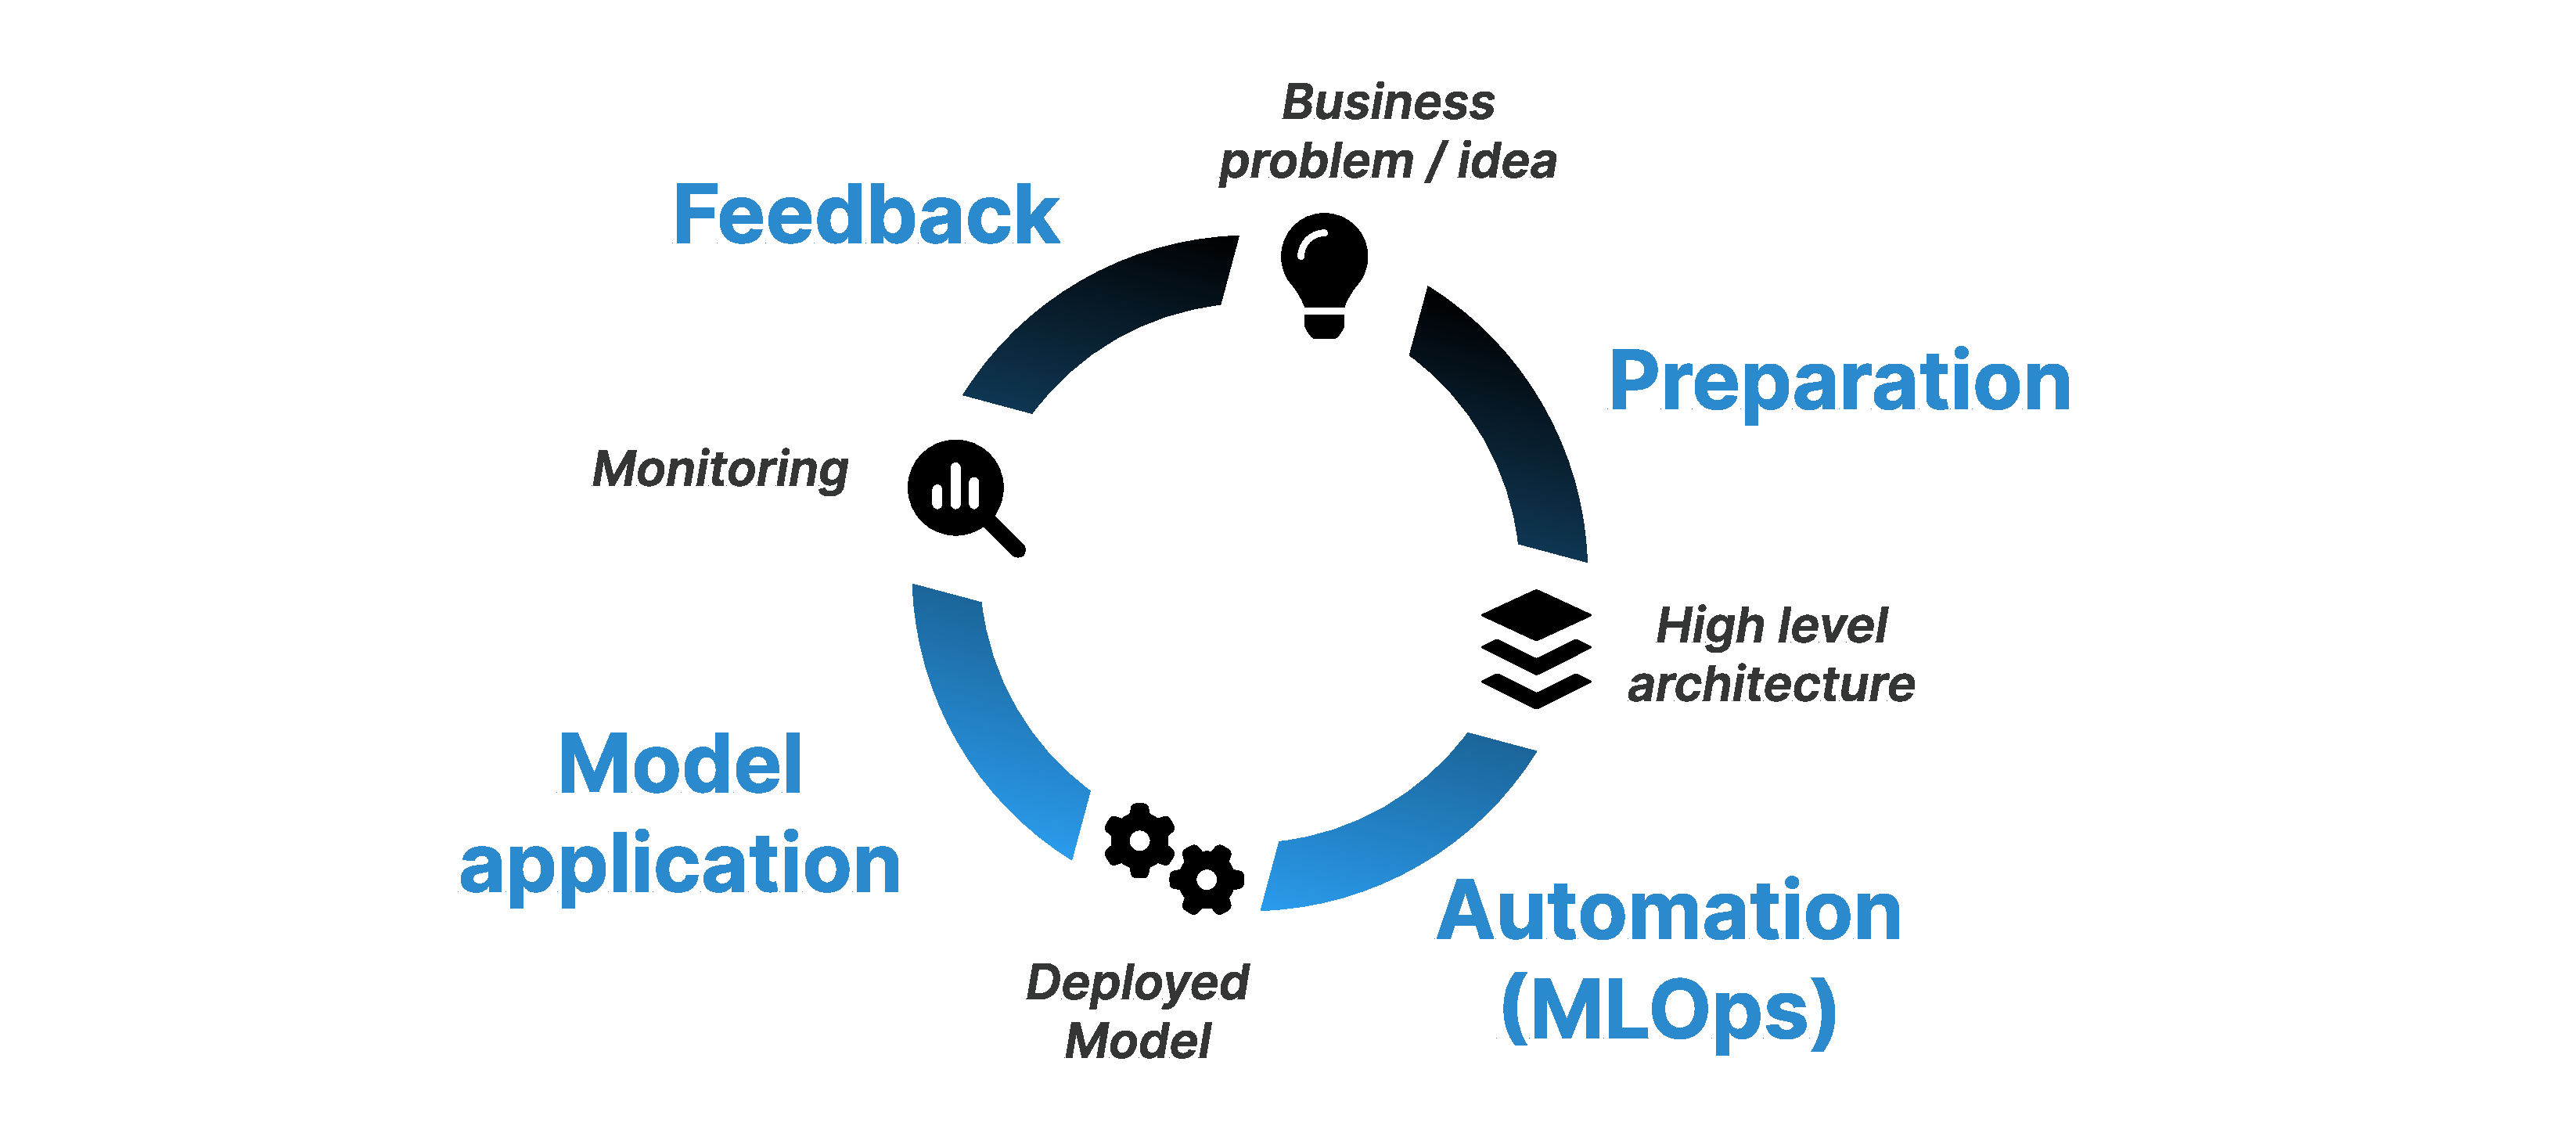
\includegraphics[width=1.0\textwidth]{figures/figure_1_4.pdf}
% \\
% \parbox[t]{\textwidth}{\vspace{1ex}\large\hspace*{7.5mm}Description}
\captionsetup{style=figureStyle}
\caption{High-level life cycle of MLOps\cite{faubel_l_2023}}\label{fig.1.4}
\end{figure}

However, everything does not always proceed according to plan, and unexpected challenges may arise. Initially, it is essential to conduct an evaluation of stakeholders via researching detailed information about them, understanding their previous activities, and scheduling a meeting with all interested parties in order to remain adaptable to the situation. After that, there is a process of aligning business objectives with stakeholders that includes the determination of specific outcomes and desired tangible business benefits (which do not necessarily have to be financial gains but rather long-term strategic, social, or other advantages). This task is typically performed by business analysts, but it might be undertaken by the team lead or any other person that is responsible for the R\&D team, considering the potential complexity of tasks that require deep expertise. During this phase, documenting any processes, systems, vital elements, or policies related to the business is critical as it can impact KPI metrics such as quality, performance, time-to-market, costs, ROS, scalability, etc. \cite{testi_m_2022}. At the same time, the limitations of project resources must be defined in terms of technological competences as well as resource boundaries (complexity, prices, and timescales). This might result in proper risk management that saves additional time and effort in advance. From a practical perspective, it is advisable to review open-source or commercial solutions in the relevant field via establishing evaluation benchmarks (any special metrics, performance, community support, or overall popularity), as they often offer superior functionality and can be further refined.

% Немного про официальные методолгии и фреймворки менеджмента в MLOps
Following the planning or initiation phase, the project transitions into active development, which is built upon the chosen development model that outlines a series of processes and approaches. For instance, the imperative model requires a progressive gain from low to high quality of the product. This approach is prevalent in data science due to the construction of hypotheses and the gradual refinement of acceptable performance. It also resembles spiral cycles, where the initial prototyping phase is rapid and subsequent iterations increase in duration and complexity. On the other hand, an incremental model is provided through small, high-quality features with audience testing for evaluation. Finally, the waterfall model involves completing all stages sequentially, resulting in a finished product. This model is suitable for small and simple projects and has modifications that include additional testing phases.

In common practice, development models serve as components of higher-level methodologies. Firstly, classic project management provides a basic toolkit in conditions of high uncertainty and strict constraints, so it could be inflexible as everything is predetermined. Secondly, the Scrum framework consists of sprints, taking into account individual tasks and previously completed tasks from past sprints. Thirdly, Kanban does not impose strict deadlines but operates as a continuous flow of tasks, typically visualized as boards representing each stage of a task's life cycle, such as 'to do', 'doing', and 'done' \cite{kim_g_2016}. Additionally, there are many other specialized approaches, such as the CRISP family, which emphasizes strict monitoring and numerous other practices \cite{shankar_s_2024, martinez_i_2021}. For example, the standard CRISP-DM (Cross-Industry Standard Process for Data Mining) was introduced by data mining experts, particularly for two teams consisting of ML scientists and ML engineers \cite{testi_m_2022}. Conversely, the CD4ML approach is only focused about the ML application lifecycle with strict phased responsibilities: data scientists handle model building and experimentation, while application developers manage model deployment and usage \cite{makinen_s_2021}. All of these methodologies are rarely applied in their pure form and often represent combinations of different approaches.





\chapter[Practical part]{PRACTICAL PART}

% \section[General review]{General review}
% - Общее объяснение концепта всей архитектуры, использованных инструментов, подходов, и концептов

\section[Web scraping]{Web scraping}
\subsection{Comparison of web scraping tools} % + краткая справка что такое web scrapping
Web scraping is the process of data extraction from various web resources. It occurs due to a request to the server from the client via HTTP or HTTPS protocols (which could be based on SSL or TLS security certificates with several HTTP versions from 1.1 to 2) to a particular domain address of the resource (that is resolved through the DNS server) or directly to the IP address. Upon completion of the TCP/IP 3-way handshake, we receive a response from the server or resource in some content format (HTML, XML, JSON, etc.). Usually, the client is represented by the capabilities of widely-used web browsers and their drivers, such as ChromiumDriver, GeckoDriver, and so on. On the other hand, the Python programming language already has a built-in package that acts as a custom client or a web toolkit - urllib (which is inherited from the http package). For example, the curl and wget packages in Linux can implement similar functionality, operating on comparable principles. The module urllib is consistently used by pip (a standard package installer for Python) to establish connections for installing packages from the PyPI (Python Package Index) registry via the setuptools package manager or precompiled packages in the wheel format. In the open-source market, the most popular solutions are custom libraries that provide greater flexibility and functionality:

- The ``requests'' library is the most popular one in this list and currently ranks in the top 10 packages on the PyPI registry. It does not support asynchronous requests or HTTP/2. Certainly, there could be a threading pool or multithreading, which depends on the number of CPU threads. In contrast, asynchronous processing operates with a single thread while still achieving concurrency. Asynchronous tasks are typically I/O-bound, whereas multithreading tasks are CPU-bound.

- In case of ``urllib3'', it is the same as ``requests'' without any new functionality.

- ``aiohttp'' is strictly focused on asynchronous requests and tasks.

- ``httpx'' is modern and capable of handling various HTTP requests across versions, supporting both asynchronous and synchronous operations.

These libraries are only suitable for static websites and may not be applied to sites with dynamically loaded content due to JavaScript code. Although, Js2Py library could solve that issue via translation from JavaScript code into Python objects accordingly, it is more appropriate to utilize dedicated toolkits like Selenium or Playwright, which allow to control browsers using Python code.

Acquiring and analyzing data from websites typically involves parsing HTML code. HTML represents a structure in the form of a Document Object Model (DOM), which makes it challenging to process using conventional methods like regular expressions. Therefore, full-fledged tools such as bs4 with lxml, parsel, or selctolax enable the extraction of elements based on names, classes, tags, CSS styles, or XPath locations. It is also important to acknowledge comprehensive frameworks like Scrapy, which can execute all the aforementioned tasks, including conducting requests and parsing simultaneously.

\subsection{General overview of web scraping part} % (Базовый парсинг данных МФЦА на httpx и bs4)
In this project, it was decided to extract data from the AIFC platform and their public registry of registered organizations. The entire structure of the data extraction pipeline is illustrated in figure 2.1.

\begin{figure}[h]
\centering
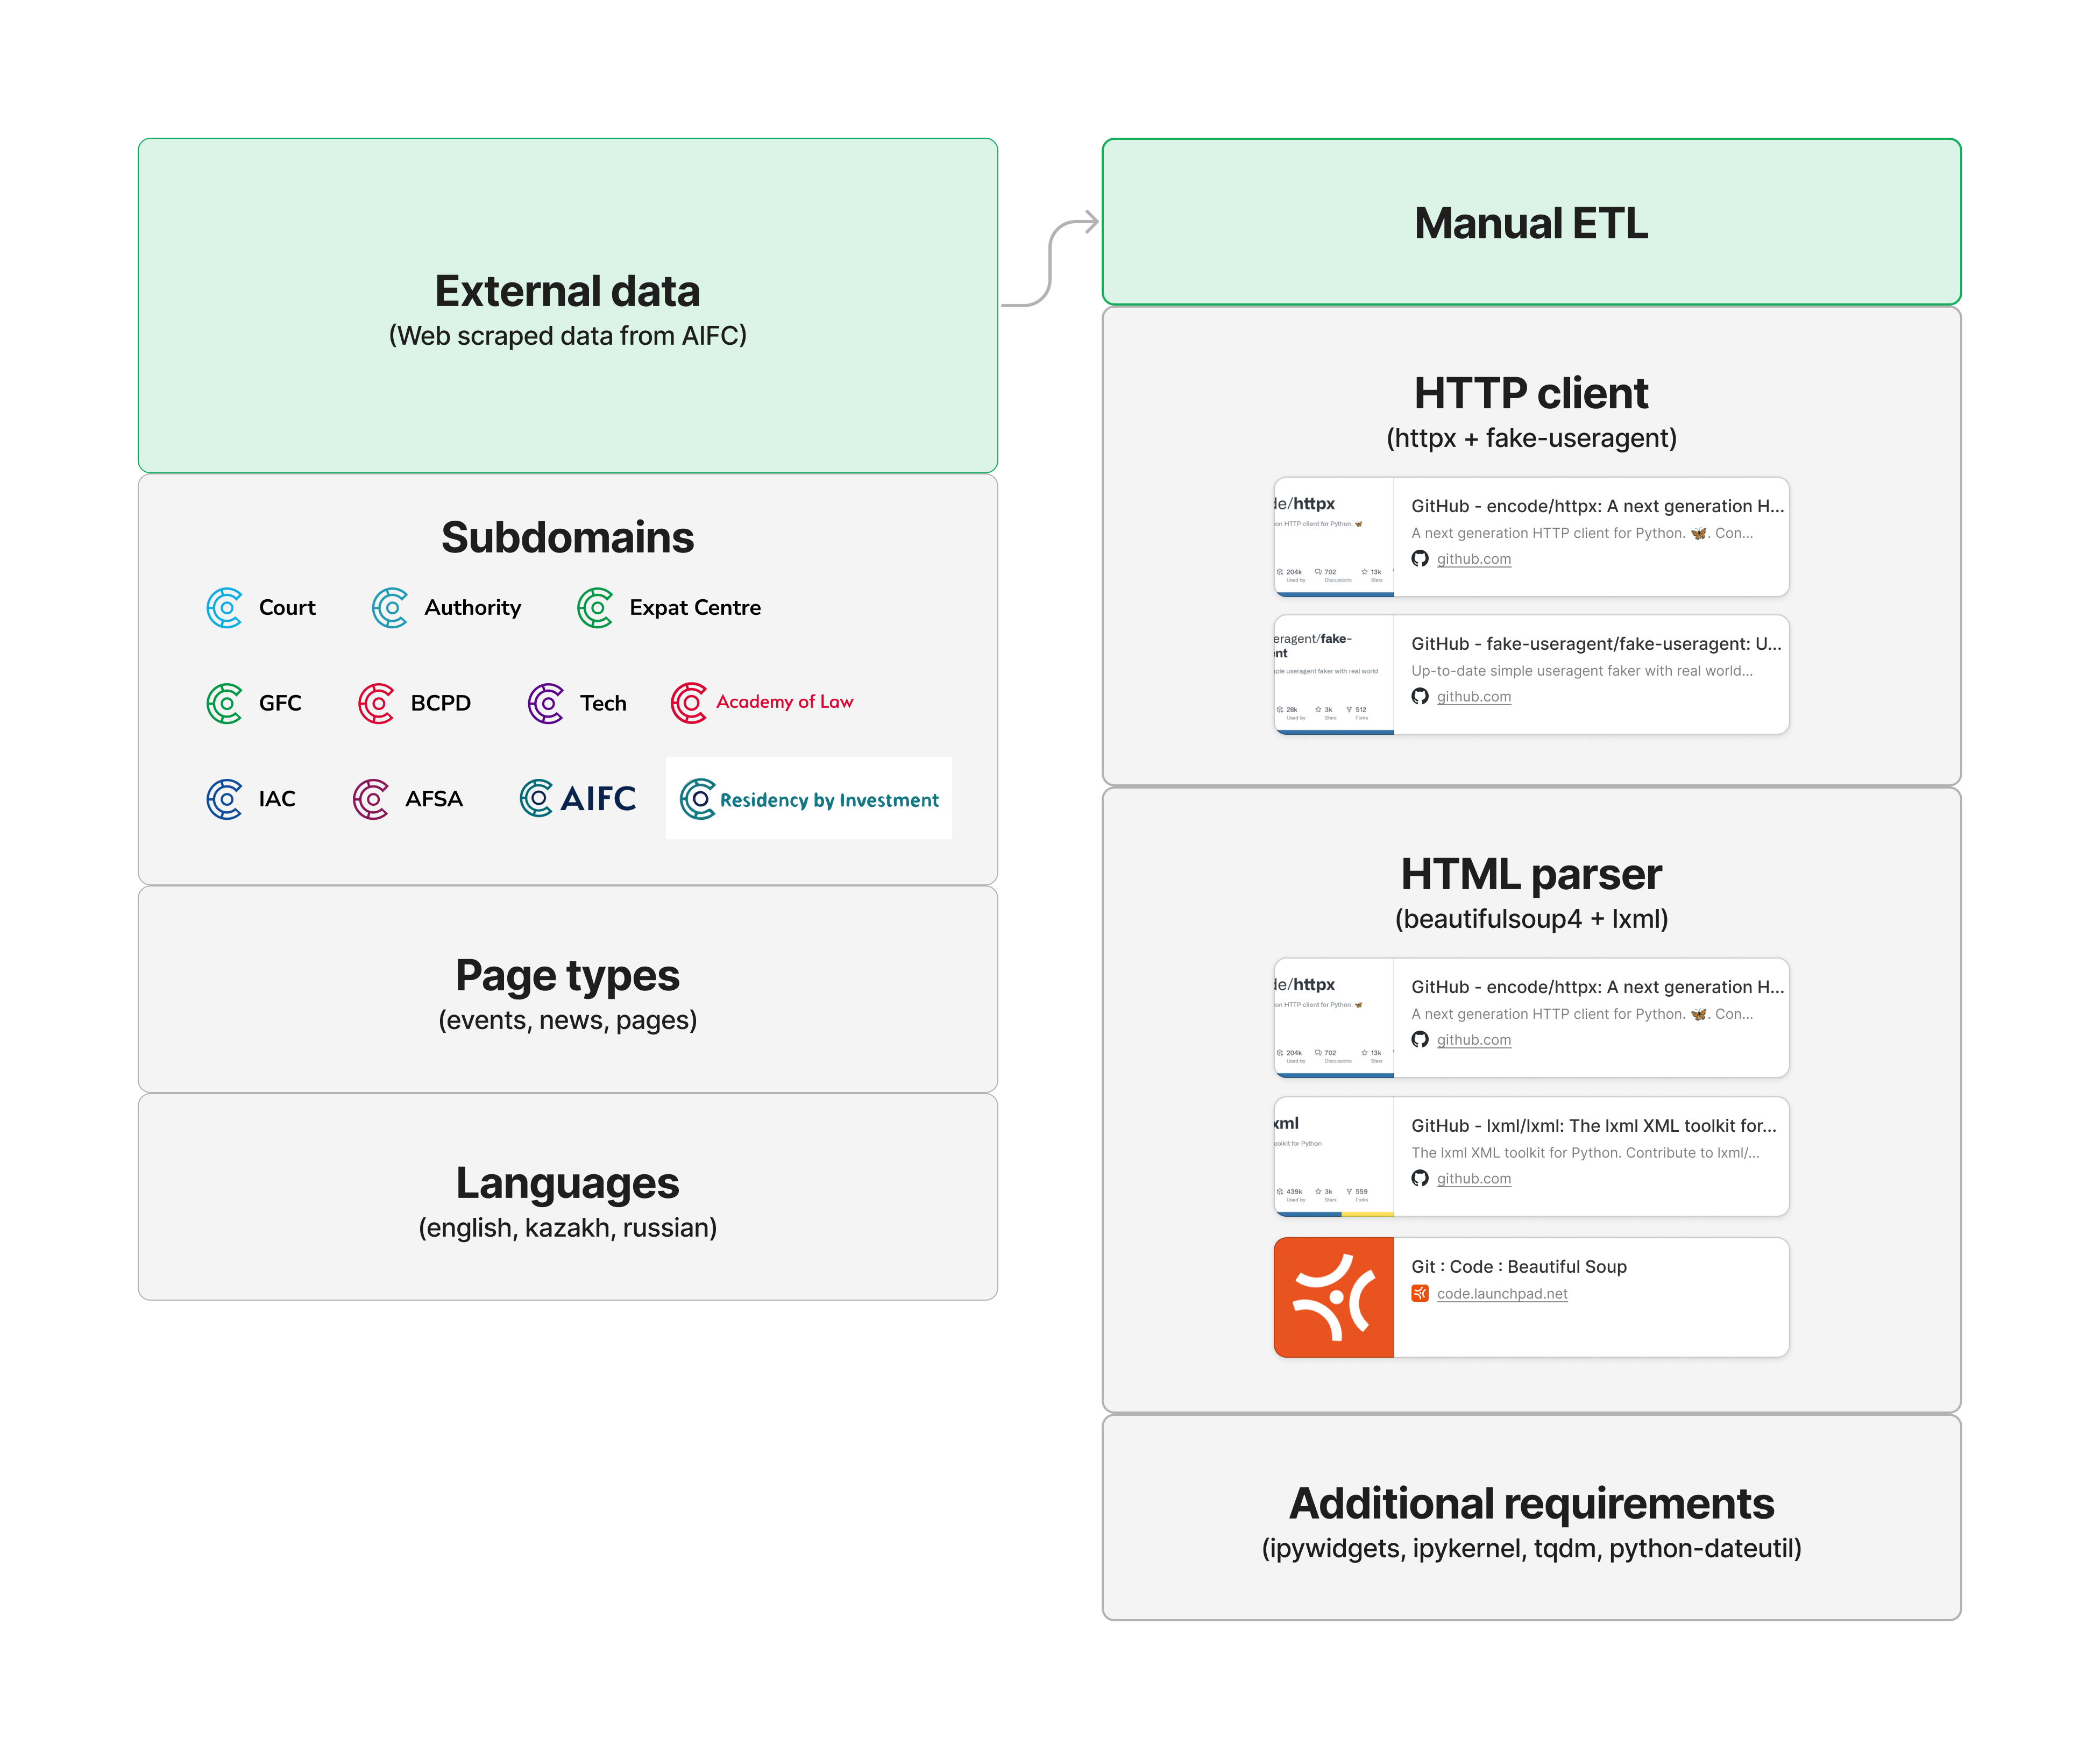
\includegraphics[width=1.0\textwidth]{figures/figure_2_1.png}
% \\
% \parbox[t]{\textwidth}{\vspace{1ex}\large\hspace*{7.5mm}}
\captionsetup{style=figureStyle}
\caption{External sources of data with provided manual ETL or web scrapping pipeline}\label{fig.2.1}
\end{figure}

Firstly, the left block that is labeled ``External data'' represents data sources, which include all AIFC subdomains except for the AIX platform. Because data on AIX is updated nearly every second, it is difficult to store it on a standard personal computer, necessitating a powerful server device. Additionally, the data was available in three languages and three general types. Secondly, the data extraction was performed using the httpx client and fake-useragent library to generate random client metadata to prevent the system from blocking requests due to excessive traffic from a single device. Additionally, proxies or VPNs can be utilized to mask the device's IP address or route requests through an intermediary device to avoid detection. Thirdly, bs4 and lxml were applied to parse the HTML tree, with the tqdm library used to display script progress in the terminal.

\subsection{Explanation of data parsing and extraction processes}
Before starting data parsing and extraction, it is essential to conduct reconnaissance in order to identify any hidden APIs that can directly provide the raw data in a structured format. Often, web applications and services fetch data from the backend, which typically returns it as JSON objects. It is an efficient and flexible method for data transmission. In this case, a hidden API was discovered by analyzing the behavior of the ``burger button class'', which reveals additional pages and endpoints on the site, functioning as a navigation menu as represented in figure 2.2.

\begin{figure}[h]
\centering
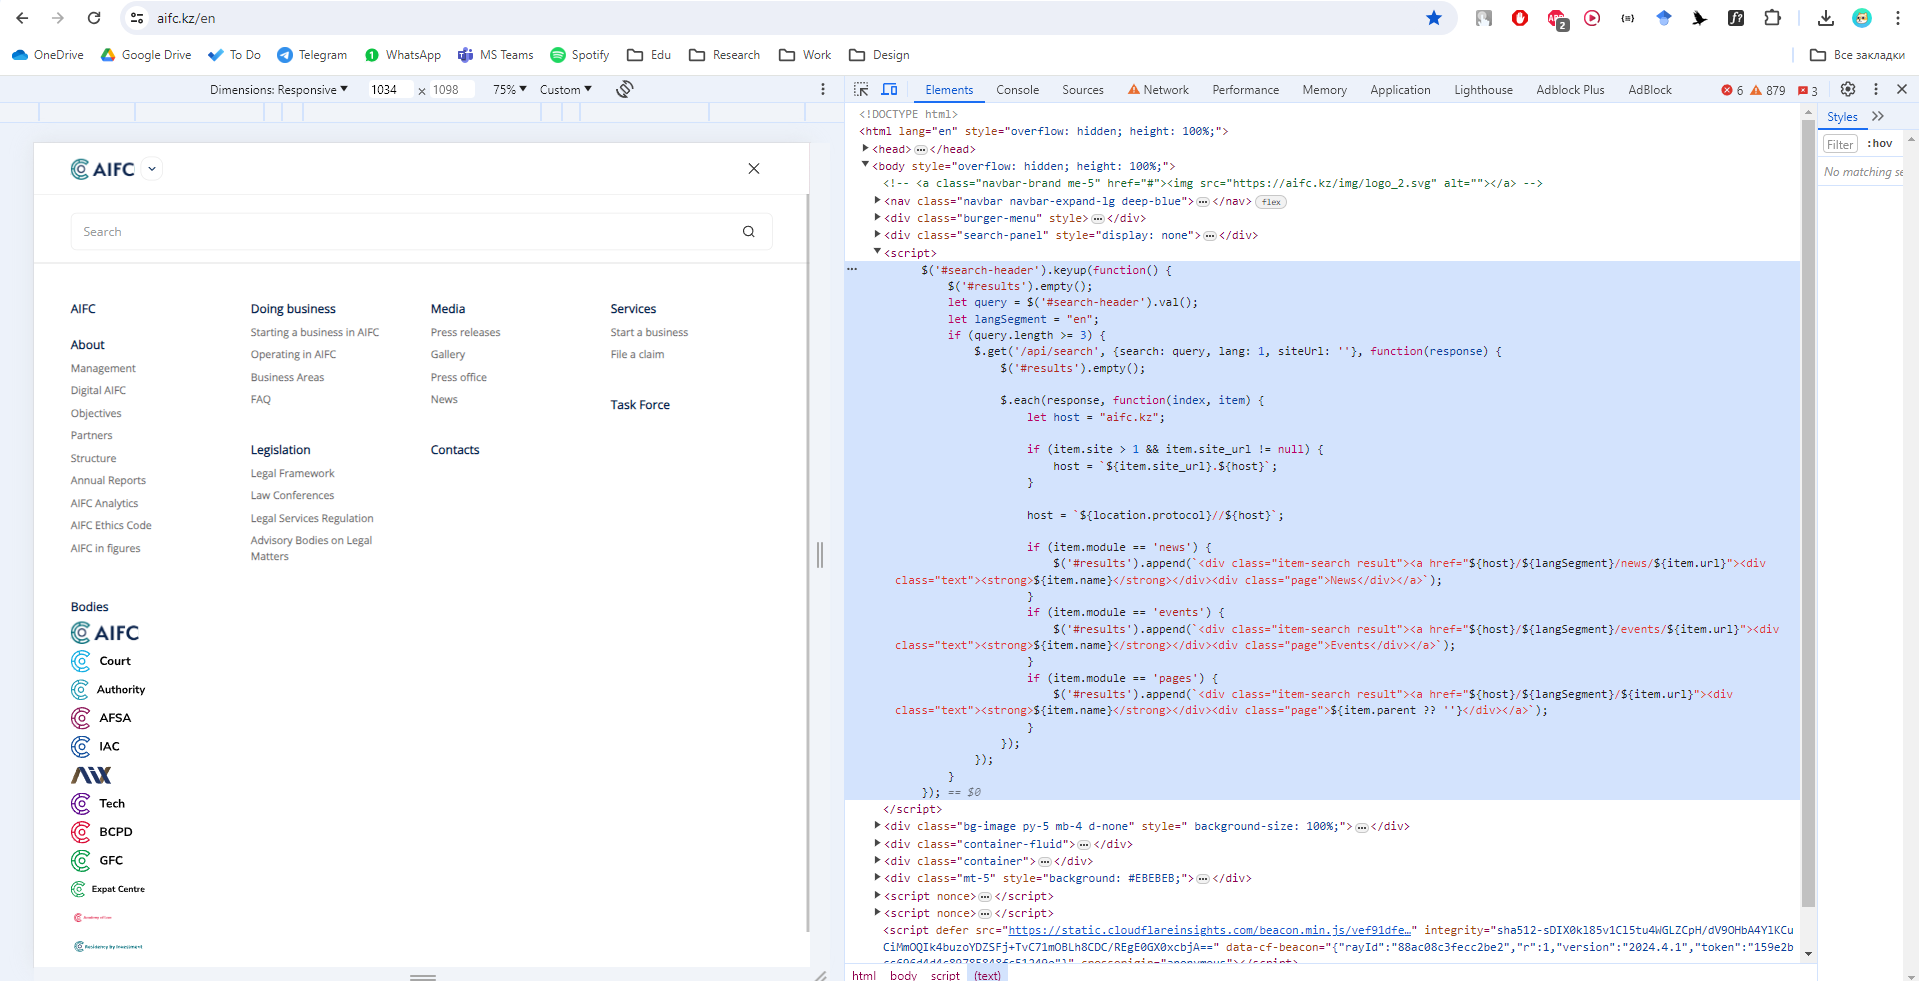
\includegraphics[width=1.0\textwidth]{figures/figure_2_2.png}
% \\
% \parbox[t]{\textwidth}{\vspace{1ex}\large\hspace*{7.5mm}}
\captionsetup{style=figureStyle}
\caption{Screenshot from Google Chrome Browser with debug console on the AIFC website}\label{fig.2.2}
\end{figure}

That element is dynamically generated by JavaScript, which sends a request to an API endpoint (``api/search'') with specific query parameters: siteUrl (determining the subdomain type, such as itrp, aifc, etc.) and lang (the resource language, where 1 is English, 2 is Kazakh, and 3 is Russian). As a result, the API returns an array of JSON objects, as shown in figure 2.3. Each object consists of the following fields: id, url, name, description, site, module, parent, and site\_url.

\begin{figure}[h]
\centering
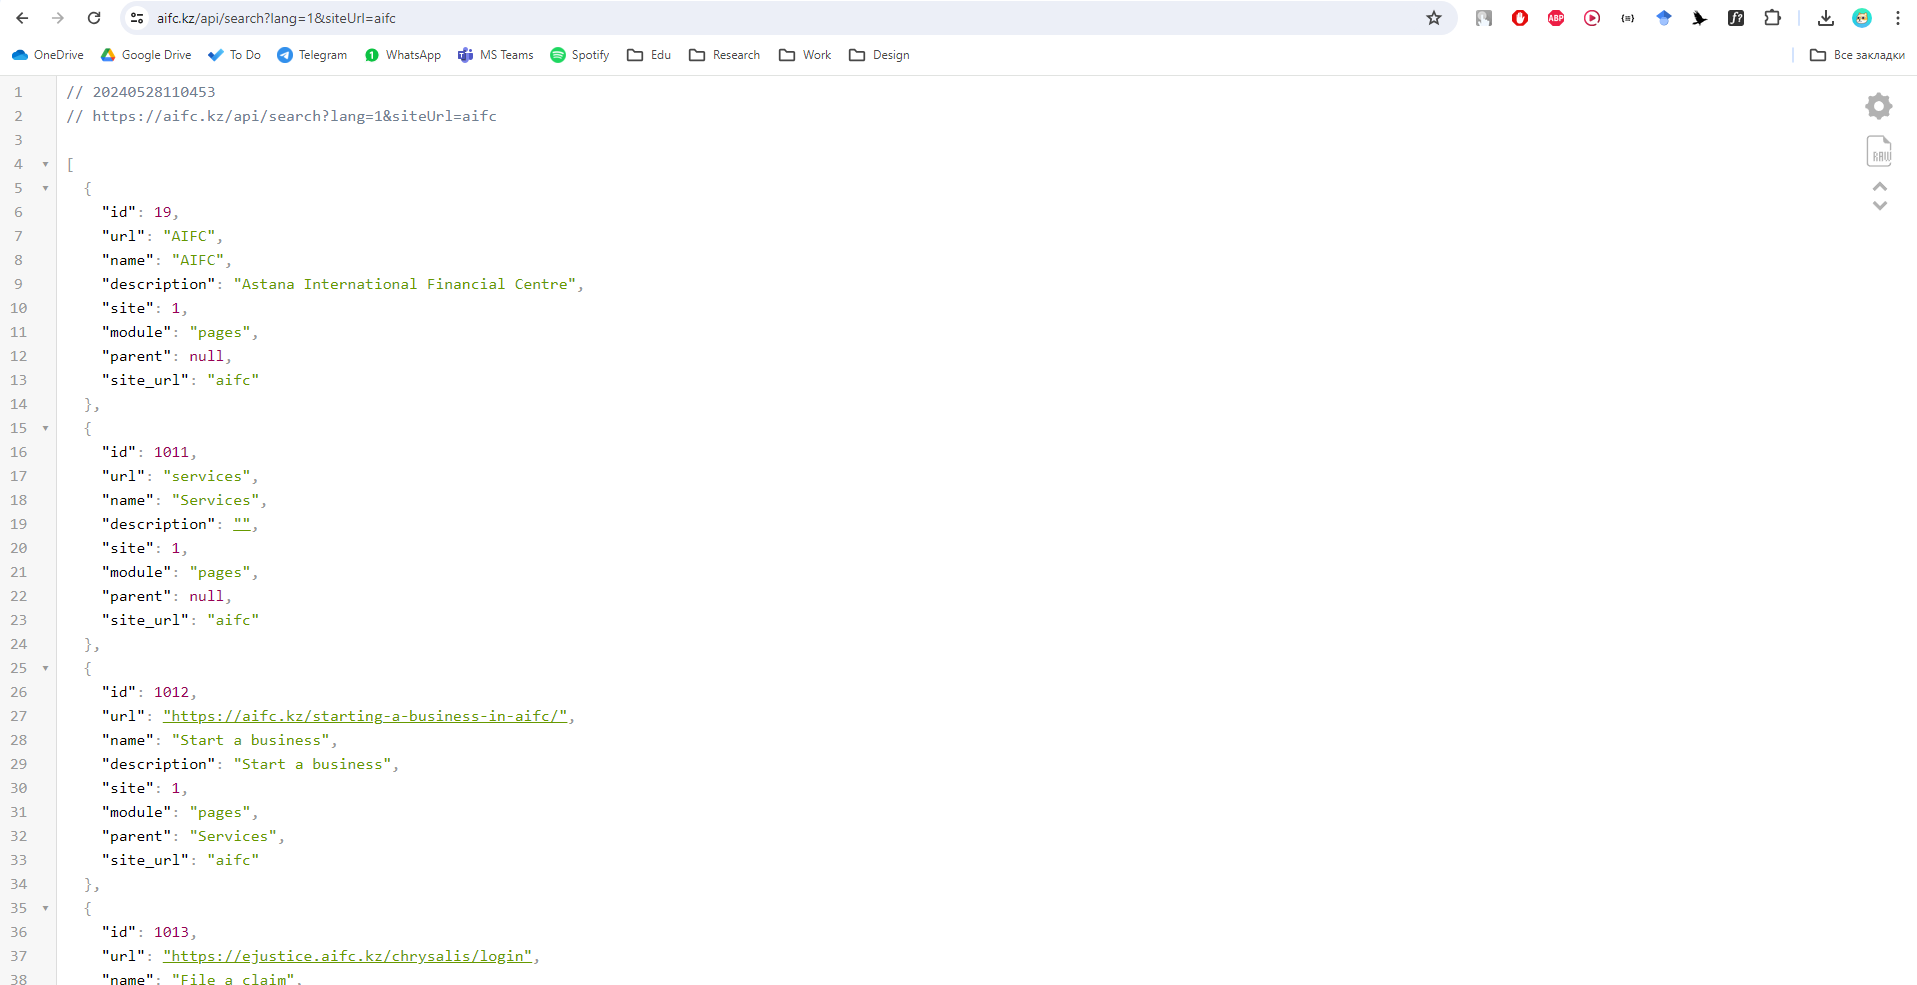
\includegraphics[width=1.0\textwidth]{figures/figure_2_3.png}
% \\
% \parbox[t]{\textwidth}{\vspace{1ex}\large\hspace*{7.5mm}}
\captionsetup{style=figureStyle}
\caption{Array of JSON objects that are returned by API with specific query parameters}\label{fig.2.4}
\end{figure}

For example, id field is a unique identifier for each record without any duplicates within the database. The url field may contain the full link or just the endpoint of the element. The name and description fields are primarily for displaying textual context and are not required for data parsing. The site field was found to be a unique domain identifier, similar to site\_url. This inconsistency suggests unorganized API design by the platform's developers and the presence of numerous redundant elements. The module field indicates the type of page, with three types identified: news (always located at the ``/news'' endpoint), events (about upcoming events at the ``/events'' endpoint), and pages (all other pages that do not fit the criteria of previous types and could be nested if a parent field is specified).

% поэтапное объяснение кода и входных данных и конечных данных
Based on this data, there were written Python scripts with a phased approach: get\_api\_json, transform\_and\_compare\_json\_files, group\_json\_files, get\_news\_data, main. Of course, it could have been implemented using object-oriented programming or something more structured; this example of a parser adequately fulfills its intended task of extracting only the required data. The complete structure of this parser and its code are described in Appendix A.

Firstly, the get\_api\_json function recursively fetches all JSON objects for all languages, grouping them into folders for en, kz, and ru, with JSON objects further grouped by their subdomain affiliation. Moreover, a custom client around httpx with an increased read timeout prevents the parser from crashing if the server takes a long time to respond. JSON object manipulation was done using Python's built-in json module and dict objects, which closely resemble JSON representations.

Secondly, the transform\_and\_compare\_json\_files function transforms the JSON files for each language by removing site\_url and site fields, leaving only objects with unique ids, and then saves the changes. Initially, this function also compared the number of objects and performed a special count. That approach significantly slowed down the data parsing process; hence, it was decided to remove this comparison.

Thirdly, group\_json\_files creates a directory in each language folder for each module type (pages, news, events), effectively grouping JSON objects.

Fourthly, for this example, only the extraction of news will be described and implemented using the get\_news\_data function, as there are already around a thousand objects, and there will be no significant difference from larger datasets. This function creates even more nested directories with folders for HTML and text for each previously parsed JSON object. It then forms the url object for each request to retrieve the original HTML and downloads and parses it using bs4 through its built-in CSS selectors. Subsequently, all downloaded data is saved to the database in embedding format using an external function. Below is the detailed file structure and its description for the final extracted data, as presented in figure 2.4.

\begin{figure}[h]
\centering

\includegraphics[width=1.0\textwidth]{figures/figure_2_4.png}
% \\
% \parbox[t]{\textwidth}{\vspace{1ex}\large\hspace*{7.5mm}}
\captionsetup{style=figureStyle}
\caption{File structure of extracted data}\label{fig.2.4}
\end{figure}

\clearpage

\section[Backend service]{Backend service}
\subsection{General overview of backend part}
% Создание структуры базового сервиса и его архитектура + Про FastAPI как основной бэкенд фреймворк и другие архитектурные и тд решения
The backend architecture is based on a modular monolith structure, where each part is divided into specific elements as feature objects (such as admin, chats, users, auth, etc.), rather than by grouping types (like folders for services, routers, etc.). This architecture does not strictly adhere to DDD (Domain Driven Design) or clean architecture principles, yet it is commonly used in Python projects due to the nature of feature-driven design. All these components are located within the ``src'' folder, which can be named differently and might have multiple nested directories, as shown in figure 2.5.  Moreover, API endpoints are listed in figures 2.6, 2.7, 2.8, and 2.9.

\begin{figure}[h]
\centering
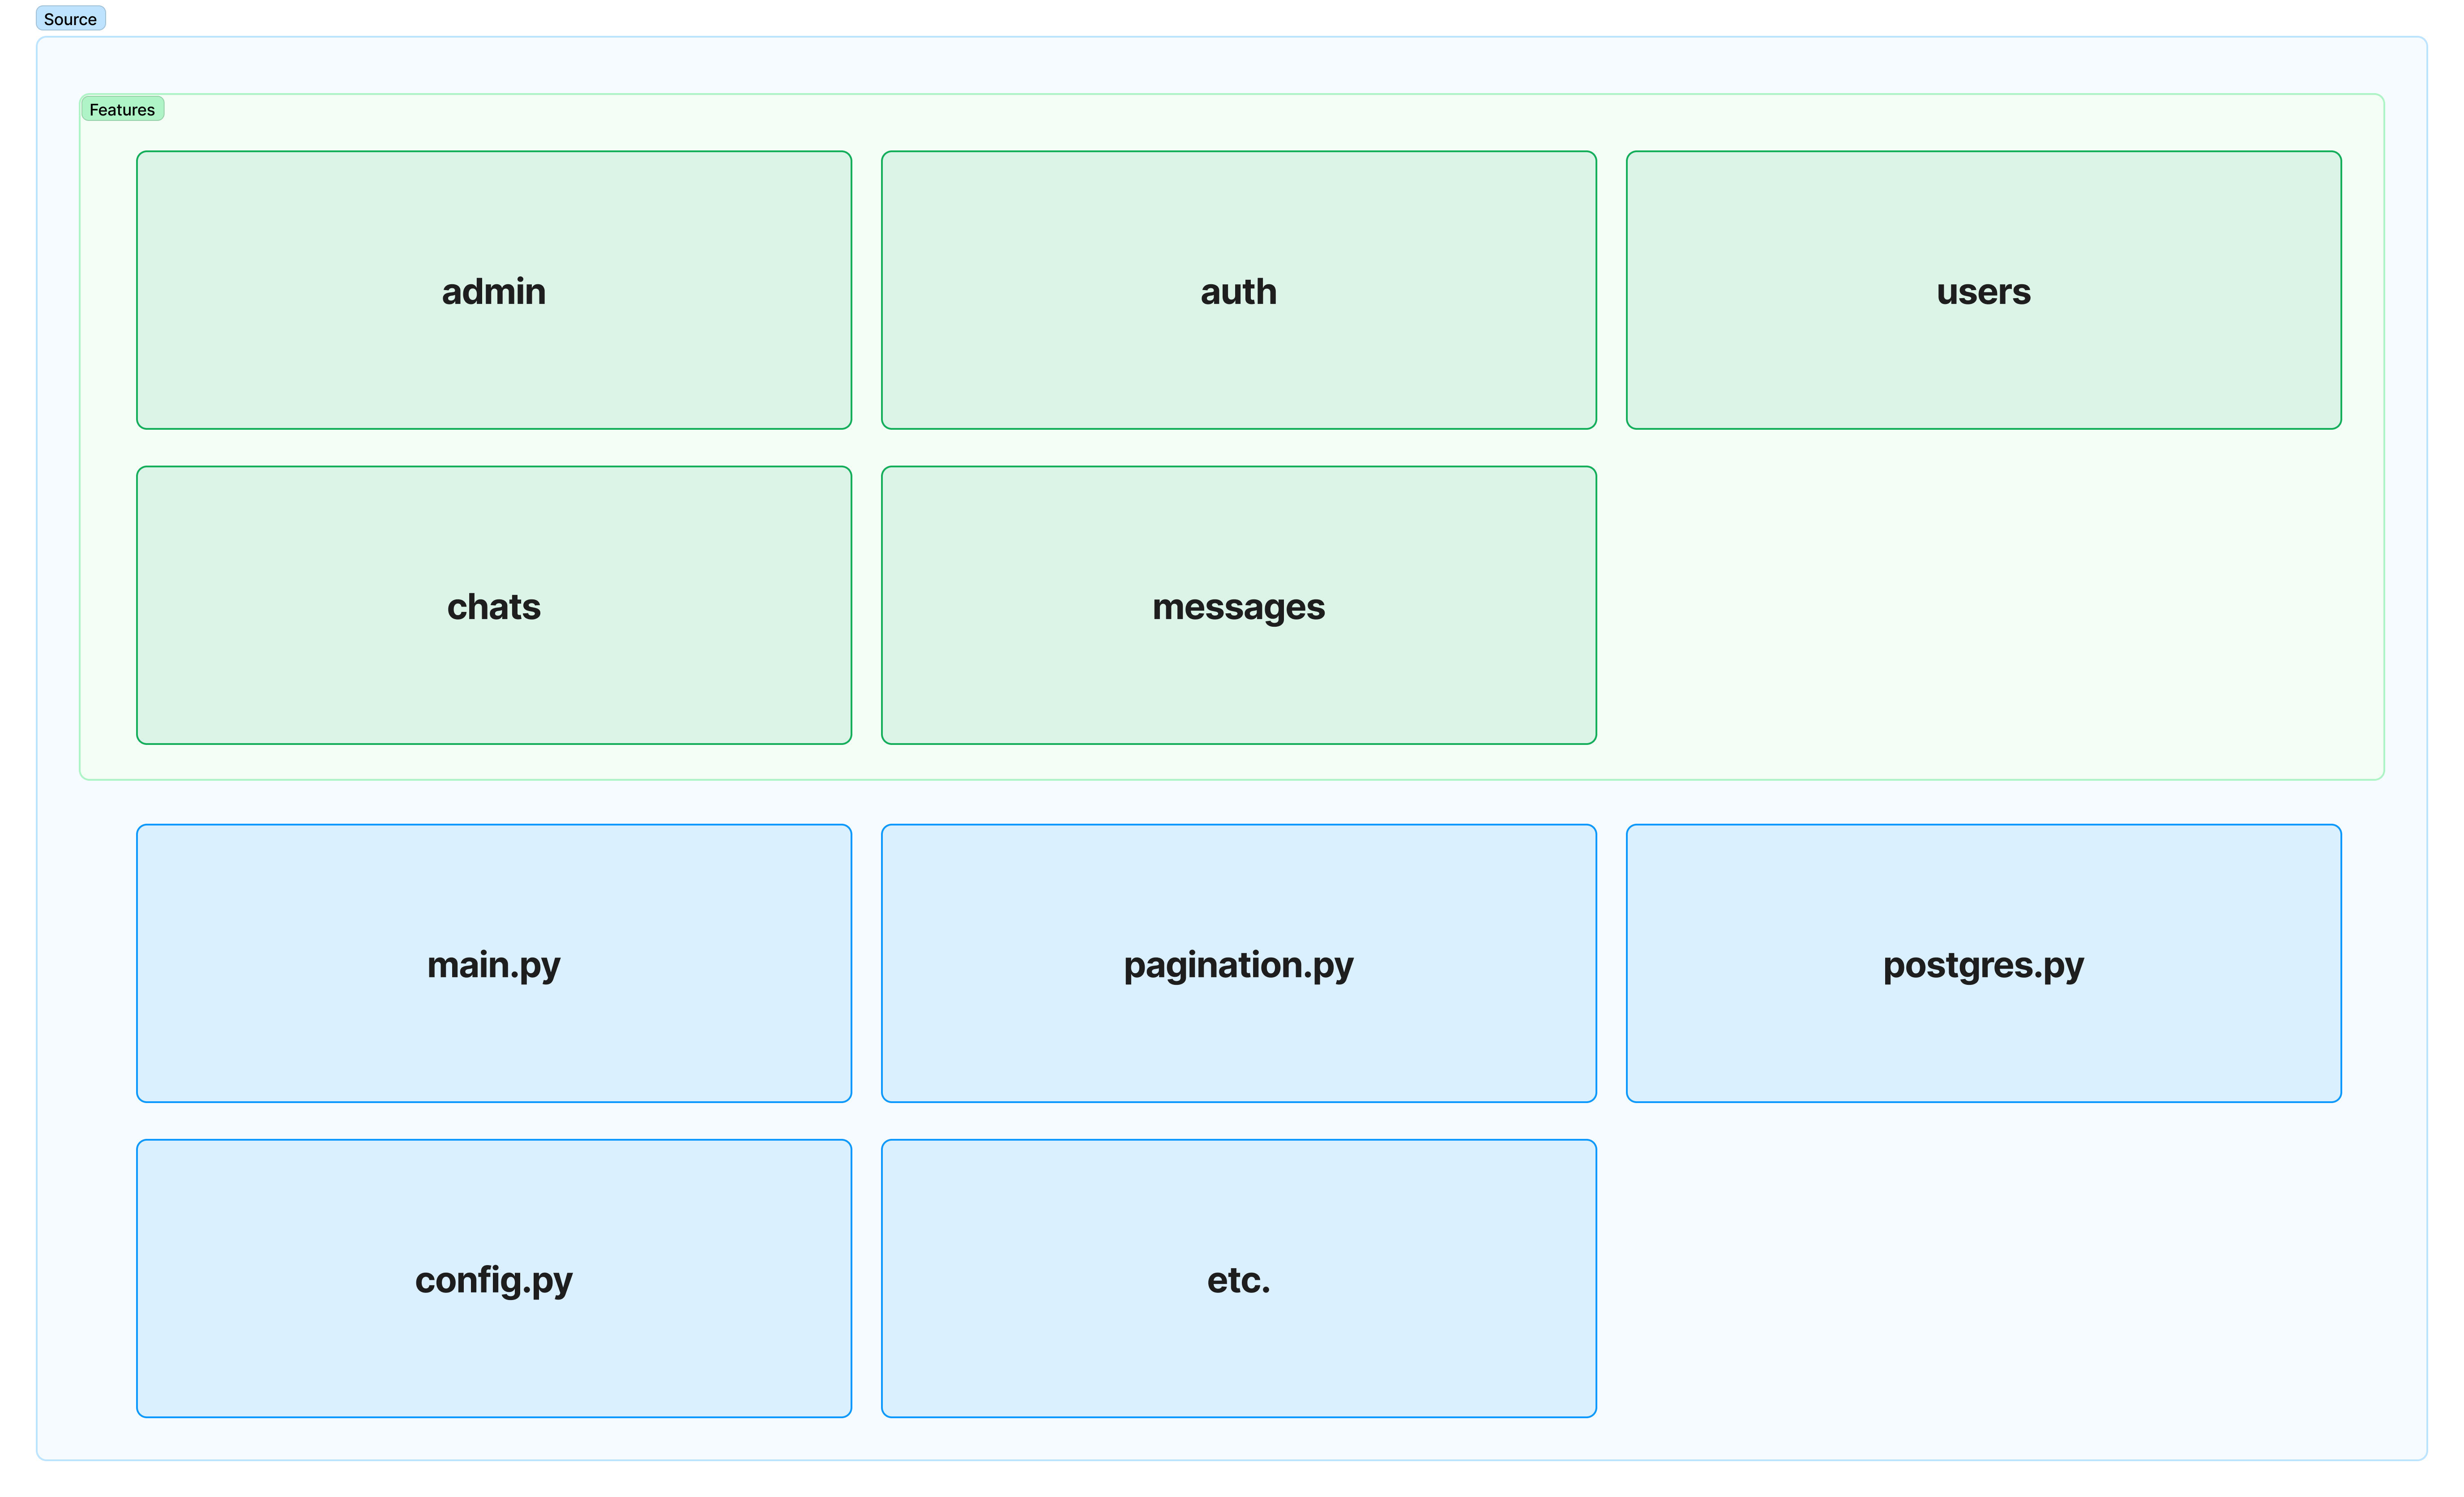
\includegraphics[width=0.85\textwidth]{figures/figure_2_5.png}
% \\
% \parbox[t]{\textwidth}{\vspace{1ex}\large\hspace*{7.5mm}}
\captionsetup{style=figureStyle}
\caption{Architecture of the backend modules or components}\label{fig.2.5}
\end{figure}

\begin{figure}[h]
\centering
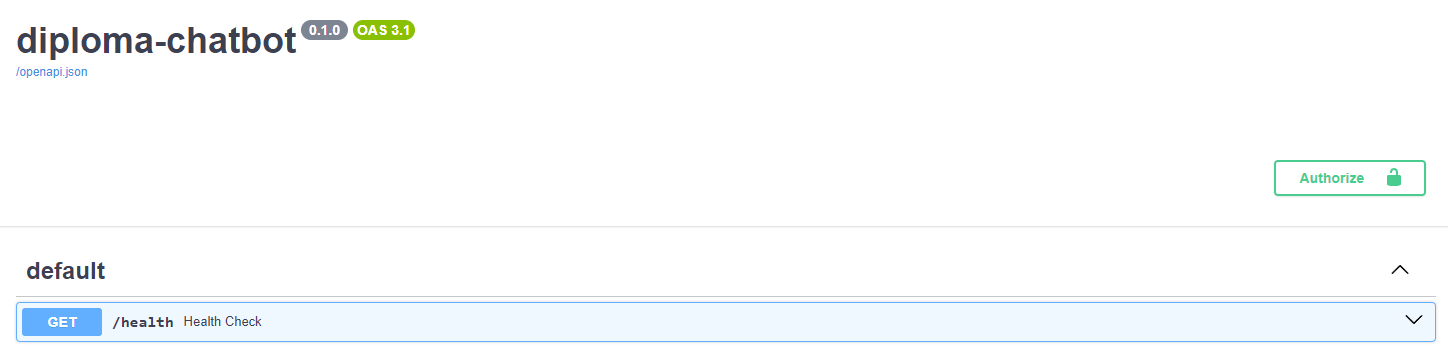
\includegraphics[width=1.0\textwidth]{figures/figure_2_6.png}
% \\
% \parbox[t]{\textwidth}{\vspace{1ex}\large\hspace*{7.5mm}}
\captionsetup{style=figureStyle}
\caption{Default endpoint for the healthcheck}\label{fig.2.6}
\end{figure}

\begin{figure}[h]
\centering
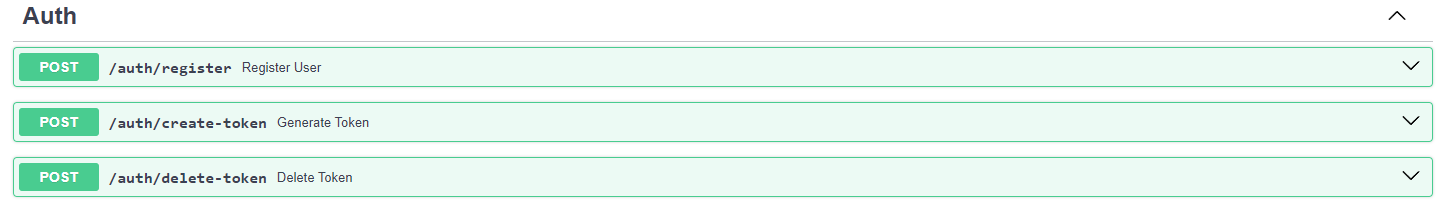
\includegraphics[width=1.0\textwidth]{figures/figure_2_7.png}
% \\
% \parbox[t]{\textwidth}{\vspace{1ex}\large\hspace*{7.5mm}}
\captionsetup{style=figureStyle}
\caption{Endpoints for the authentication process}\label{fig.2.7}
\end{figure}

\begin{figure}[h]
\centering
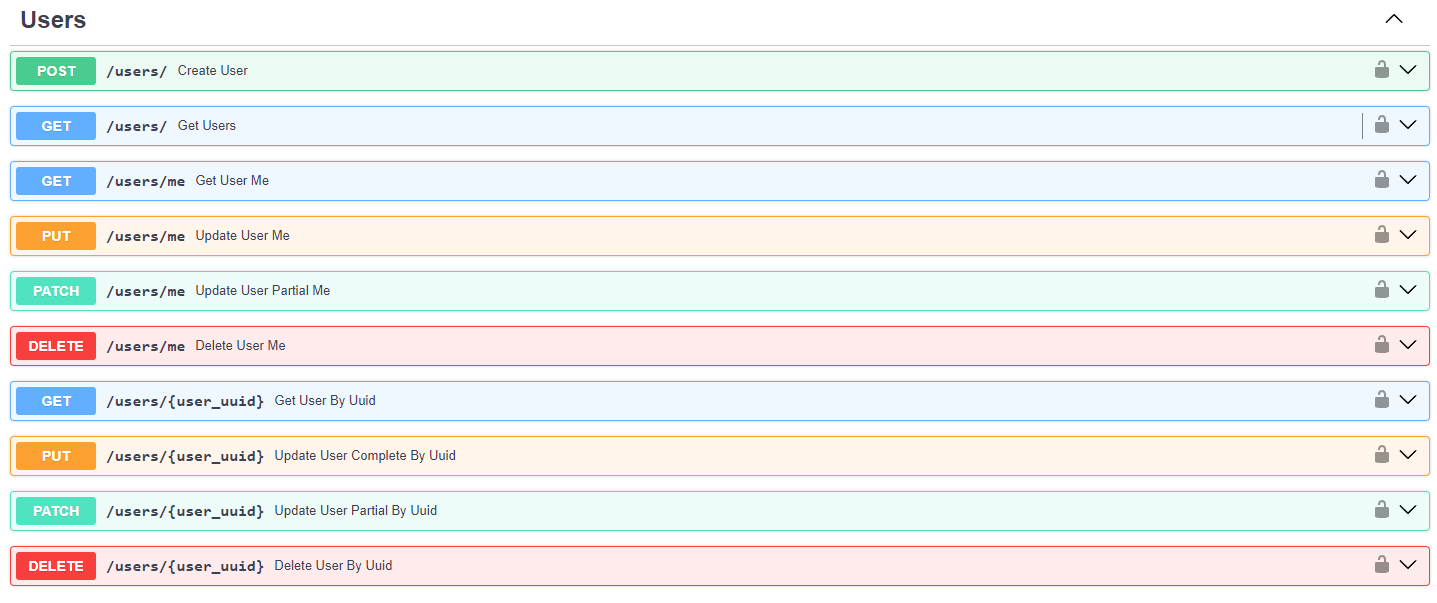
\includegraphics[width=1.0\textwidth]{figures/figure_2_8.png}
% \\
% \parbox[t]{\textwidth}{\vspace{1ex}\large\hspace*{7.5mm}}
\captionsetup{style=figureStyle}
\caption{Endpoints for the users management}\label{fig.2.8}
\end{figure}

\begin{figure}[h]
\centering
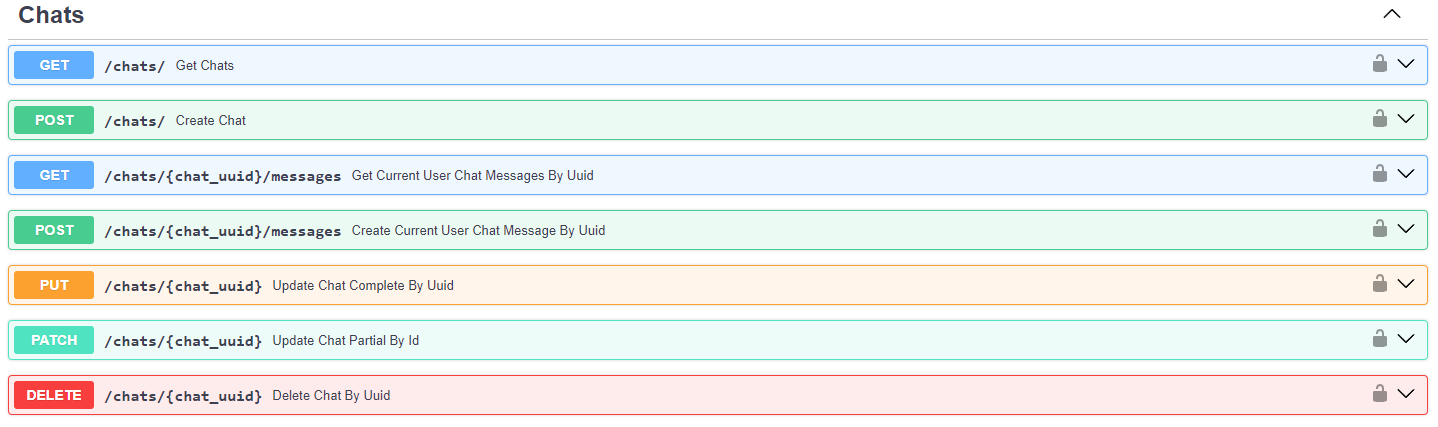
\includegraphics[width=1.0\textwidth]{figures/figure_2_9.png}
% \\
% \parbox[t]{\textwidth}{\vspace{1ex}\large\hspace*{7.5mm}}
\captionsetup{style=figureStyle}
\caption{Endpoints for the chats and messages interaction}\label{fig.2.9}
\end{figure}

Additionally, outside of the modules in src, there are auxiliary Python files along with our application's entry point, main.py, from which the application is launched. For the backend, it was decided to focus on a lightweight framework. Among the most popular frameworks in this range are FastAPI and Flask. For example, FastAPI is based on another framework, Starlette, and offers many additional features with built-in Pydantic support, as revealed in figure 2.10, which displays the entire project structure. Some code snippets are provided in Appendix B.

\begin{figure}[h]
\centering
\includegraphics[width=1.0\textwidth]{figures/figure_2_10.png}
% \\
% \parbox[t]{\textwidth}{\vspace{1ex}\large\hspace*{7.5mm}}
\captionsetup{style=figureStyle}
\caption{The project structure with the backend part}\label{fig.2.10}
\end{figure}

\subsection{Designing database models}
Generally, most databases or database management systems (DBMS) are divided into two categories:

- SQL (``Relational DB'') that typically store data with a consistent structure that does not change over time.

- NoSQL (``Not Only / Non-relational DB'') which is a common for an e-commerce store with products, each having unique properties.

To interact with DBs/DBMSs, there are specific client libraries known as DBAPIs (Database APIs) that act as interfaces or drivers. It is important to understand that all these libraries perform the same fundamental task by sending formulated query to the database. The difference lies in the interface they provide (the classes and functions available for creating queries) and whether they support asynchronous or synchronous query execution. For instance, several connection libraries are available for PostgreSQL in Python: psycopg3, psycopg2, and asyncpg. Additionally, there are various custom wrappers for database objects that enable working with native Python objects instead of raw SQL. These include "Mappers" that help to prevent SQL injection and abstract away the specifics of the DBMS when writing queries:

- ORM (Object-Relational Mapping): SQLAlchemy, Django ORM, SQLModel.

- ODM (Object-Document Mapping), dialect addons, and so on.

For example, figure 2.11 illustrates the relationships between users, chats, and messages, primarily showcasing many-to-one connections between these entities in the production DB.

\begin{figure}[h]
\centering
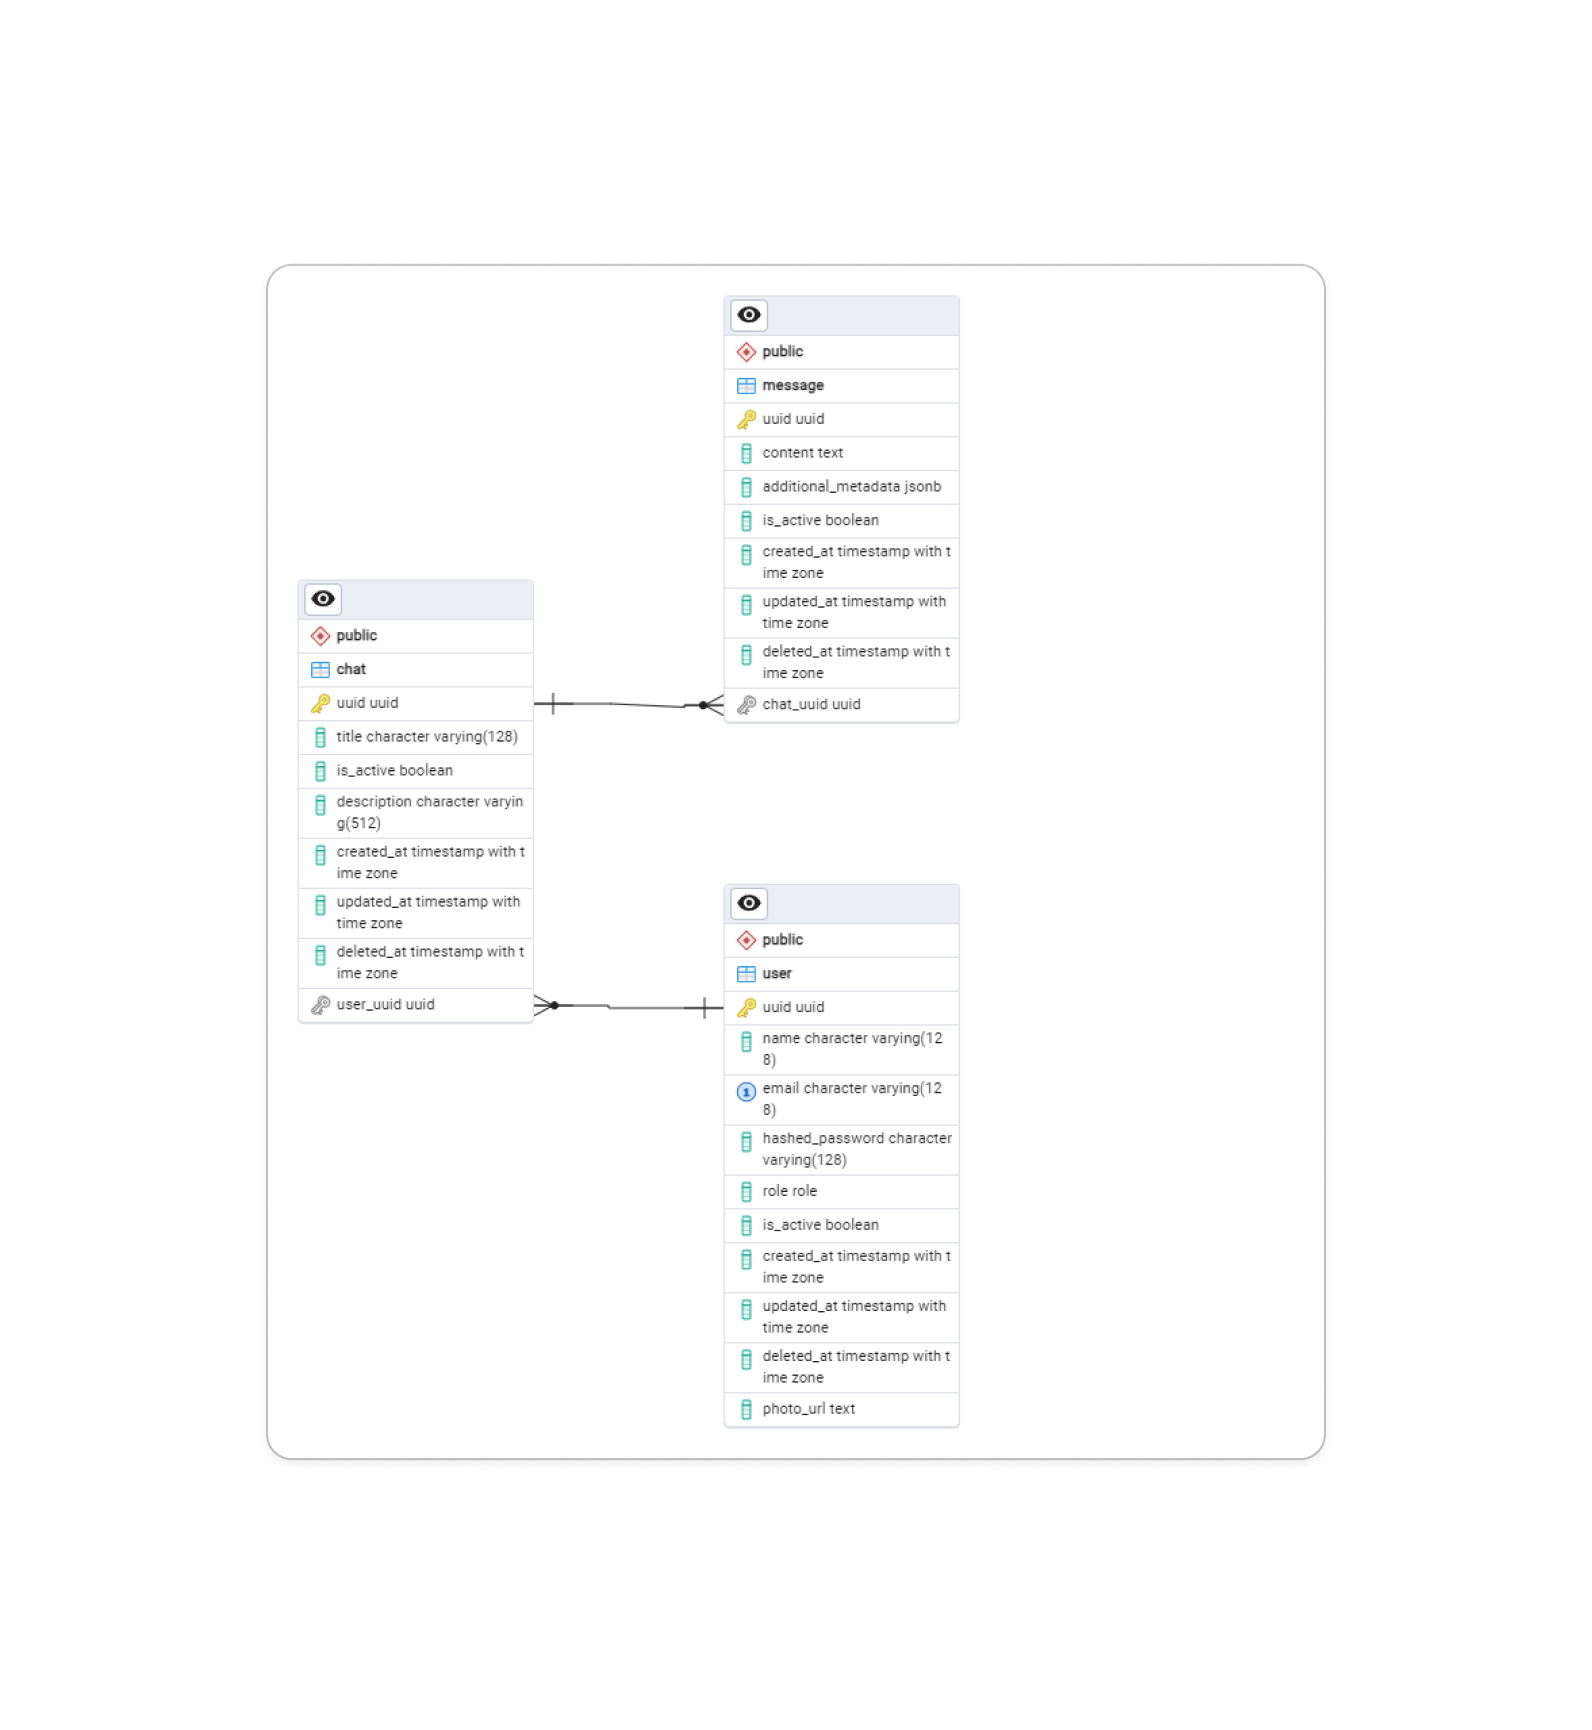
\includegraphics[width=1.0\textwidth]{figures/figure_2_11.png}
% \\
% \parbox[t]{\textwidth}{\vspace{1ex}\large\hspace*{7.5mm}}
\captionsetup{style=figureStyle}
\caption{Relations within the production DB}\label{fig.2.11}
\end{figure}

Furthermore, establishing a direct connection to the database is necessary. Therefore, in a separate file such as ``database.py'' or `postgres.py'' an asynchronous connection session is declared using ``get\_async\_session'' or ``get\_db''. In this case, a yield generator plays a crucial role in maintaining the connection within the context of a single transaction. A transaction in this context refers to one or more actions or changes in the database, such as select, update, insert, or delete operations. If even one of these queries fails or an error occurs on the database side, the changes are rolled back, and the connection is ultimately closed. This file handles the database connection, in this case, PostgreSQL. However, sometimes developers do not merely write functions in this file but wrap them into a comprehensive class like ``DatabaseHelper''.

However, interacting with the database will be impossible without loading the previously mentioned models into it. This is where the concept of migrations comes into play (version control for the database or the process of changing the database schema). For example, Alembic is a tool for managing migrations for SQLAlchemy. There has to be generated a migrations directory with the command ``alembic init migrations'', configured all settings, and created the first migration file with ``alembic revision --autogenerate -m 'Description of changes'''.

\subsection{Developing an authentication and authorization system}
Access control involves ensuring and distributing access rights or permissions within a specific environment: registration (creating new user record), identification (determining the user’s identity), authentication (verifying the user's identity / providing proof of identification), authorization (granting access rights or privileges to a resource or the entire web service following the authentication process). 

Firstly, users were divided into specific roles using RBAC (Role-Based Access Control), with a separate column in the database represented as an ENUM (a strict set of predefined values): USER, MODERATOR, ADMIN. However, in larger applications or systems, many-to-many relationships between user objects and roles are often implemented, along with adding a special JSON field for permissions. There was a custom wrapper that is implemented over the PyJWT library to implement the logic of personalized tokens or unique identifiers, which are tied only to specific users. The token is used for user identification and authentication, providing access to certain resources, as outlined in figure 2.12 and 2.13.

\begin{figure}[h]
\centering
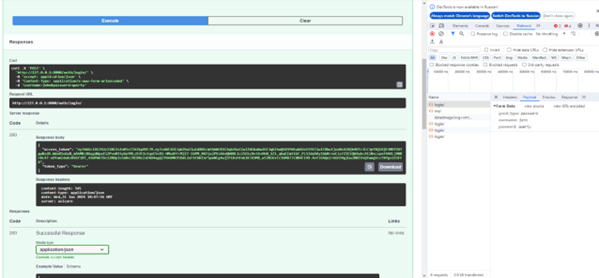
\includegraphics[width=0.8\textwidth]{figures/figure_2_12.png}
% \\
% \parbox[t]{\textwidth}{\vspace{1ex}\large\hspace*{7.5mm}}
\captionsetup{style=figureStyle}
\caption{Example of JWT access token}\label{fig.2.11}
\end{figure}

\begin{figure}[h]
\centering
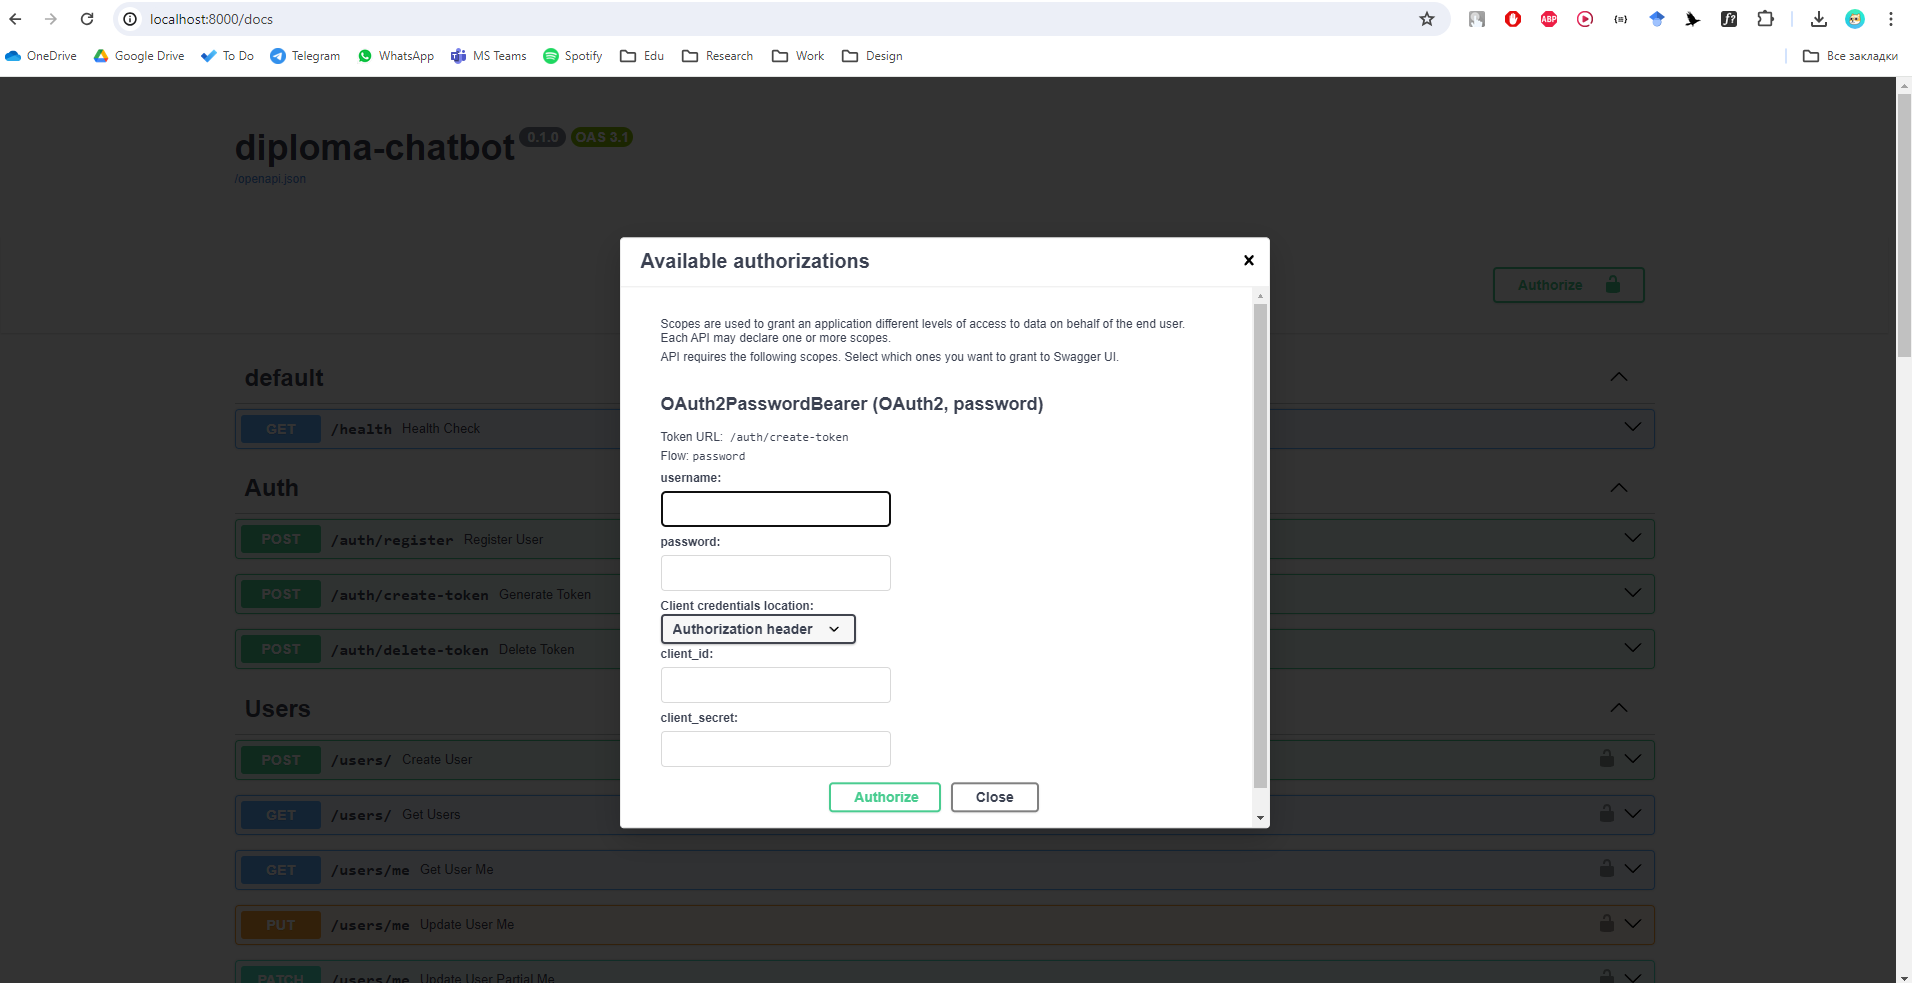
\includegraphics[width=1.0\textwidth]{figures/figure_2_13.png}
% \\
% \parbox[t]{\textwidth}{\vspace{1ex}\large\hspace*{7.5mm}}
\captionsetup{style=figureStyle}
\caption{Authentication via API documentation}\label{fig.2.12}
\end{figure}

The obtained user session token is necessary for prolonged access to platform resources; otherwise, the user would have to repeatedly log in to their account. Storing the token itself can be organized at various levels, such as browser headers, cookies, within the system's database, and so on.

Secondly, it is important to ensure that password storage adheres to commonly accepted specifications for hashing and encryption methods. Hashing involves the process of transforming data from its original form into a fixed set of characters using hash functions. In the diploma project, it is decided to utilize the modern Argon2id algorithm, which far surpasses the older Bcrypt. This process enabled us to store data in an encrypted form, making it less vulnerable to unauthorized access and hacking.

Thirdly, efforts to enhance security continued, leading to the exploration of various methods for validating input data fields (such as passwords, usernames, and other data). Two implementations for password validation were tested: through if-statements and specialized regular expressions (regex). Essentially, they do not differ, but writing regular expressions helps reduce unnecessary lines of code and avoids confusion among developers. Additionally, potential application of the Shannon Entropy formula for assessing password strength was tested. Moreover, the issue of ReDoS (Regular expression Denial of Service) was addressed in accordance with OWASP standards.

Fourthly, a special dependency was added to validate the role for each application router. This principle operates by invoking the validation function through ``Dependency Injection'' in FastAPI. This means that there is no need to manually call the function or any other method within the router's logic; it will be automatically triggered in by the framework itself.

\subsection{Integration of LLM functionality}
% Экосистема интеграции LLM или любого другого NLP-oriented решения (те же SLM или других около-трансформерных решений)
% 1 - причина использования on-premise решения вместо готовых API SaaS и cloud
Integration of LLMs or NLP products became a major trend in 2024. Businesses set themselves the task of effectively applying LLMs to their use cases and achieving efficient scalability of this solution. Consequently, the market for various LLM solutions became oversaturated relative to demand. Following the release of GPT-3.5 from OpenAI in late 2022, numerous companies emerged offering ready-to-use APIs such as Cohere, Antropic, Mistral, etc. Many commercial organizations often select these ready-made solutions because they do not require the presence of data scientists or any other ML specialists in the company, and a backend developer or DevOps engineer can easily integrate such APIs. Additionally, cloud providers and hosting services, like Microsoft Azure, offer APIs similar to OpenAI's. Conversely, some organizations focus on integrating on-premise LLM solutions or other large models, due to strict information security policies prohibiting the disclosure of any data under NDA (Non-disclosure agreement) or corporate secrets to third parties. Such companies may include cybersecurity firms, government agencies, large corporations, and many others.

% 2 - сложности интеграции on-premise решения
However, when choosing an on-premise solution, numerous challenges arise immediately. This process is slowed down for several reasons. Firstly, there is a clear issue of the high cost of computational accelerators and resources (such as GPUs, TPUs, CPUs). Consequently, scaling such a solution is also more expensive. Secondly, the company needs to hire or train experts with minimal data science competencies capable of deploying local solutions. Thirdly, according to many metrics, open-source LLM models are behind proprietary solutions.

% 3 - как упростить интеграцию on-premise решения
For instance, in order to improve model selection, it is best to rely on open metrics or benchmarks from platforms like Hugging Face's LLM-Perf Leaderboard, Open LLM Leaderboard, Chatbot Arena Leaderboard, Bigcode Models Leaderboard, and many others. Additionally, conducting proprietary research and metrics is essential. However, addressing the issue of large models and high load can be resolved in several ways:

- The simplest approach is to use smaller models like Small Language Models (SLMs), which typically have up to 3 billion parameters on average, or basic transformer-based encoders / decoders such as GPT2, T5, BERT, and their variations and modifications. Model size is relative to the number of weights and parameters, with modern LLMs ranging from 7 billion to over 70 billion parameters. Therefore, this approach can indeed be helpful, as not all tasks require large LLMs, and it may be possible to address the task by breaking it down and solving it selectively with other models or approaches, thus avoiding obvious over-engineering.

- Another approach could be fine-tuning for a specific domain or task type. There are numerous types and directions of fine-tuning, including adapters, additive, selective, parameterization-based, soft, etc. However, some studies note that fine-tuning can degrade the model in certain cases because the original pretraining dataset lacked some data patterns, leading to hallucinations in the model or significantly narrowing its capabilities in other tasks where it is not retrained. 

- An alternative strategy for optimizing could involve quantization and reshaping the model format. Quantization changes the model format and affects the floating-point precision - essentially, the lower the precision, the lower the quality of the outputs since it relies on matrix or tensor computations under the hood, as in Numpy or Pytorch. On the other hand, conversion or compilation or compression can also be integrated with quantization and is very similar to it, often presented in various transformed formats like GGML, GGUF, AWQ, GPTQ, etc.

% что было сделано по итогу кратко
For this project, the Llama 3 model with 8 billion parameters in an 8-bit quantization format was chosen. To run the model locally, a specialized inference server or driver is required. For example, there are numerous options tailored to different inference algorithms - vllm, llama cpp, are low-level, while ollama, llama cpp python server, etc., are high-level ones. API from the llama cpp python server provides full compatibility with the OpenAI API specification locally for any model, as shown in figures 2.14, 2.15, 2.16, and 2.17.

\begin{figure}[h]
\centering
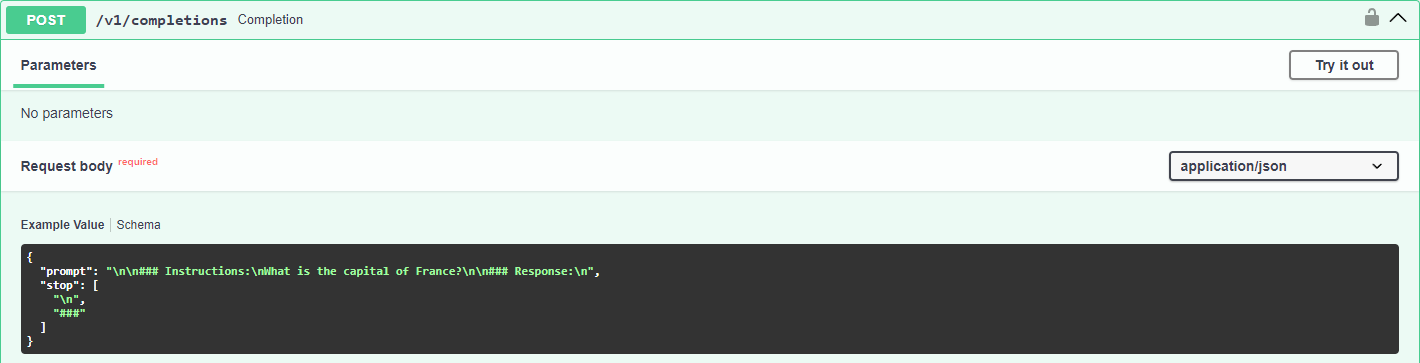
\includegraphics[width=0.6\textwidth]{figures/figure_2_14.png}
% \\
% \parbox[t]{\textwidth}{\vspace{1ex}\large\hspace*{7.5mm}}
\captionsetup{style=figureStyle}
\caption{Endpoint /v1/completions with POST method to generate completion of records based on examples}\label{fig.2.14}
\end{figure}

\begin{figure}[h]
\centering
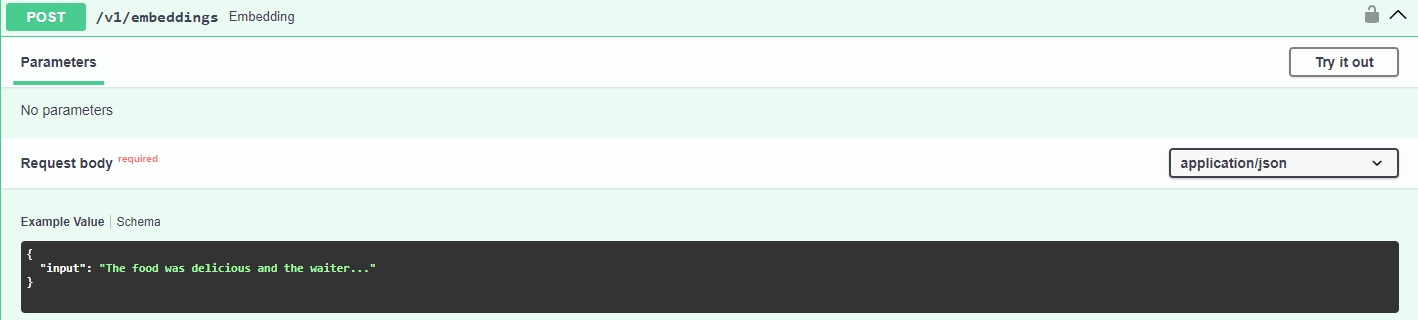
\includegraphics[width=0.6\textwidth]{figures/figure_2_15.png}
% \\
% \parbox[t]{\textwidth}{\vspace{1ex}\large\hspace*{7.5mm}}
\captionsetup{style=figureStyle}
\caption{Endpoint /v1/embeddings with POST method to generate vector embeddings for specific text}\label{fig.2.15}
\end{figure}

\begin{figure}[h]
\centering
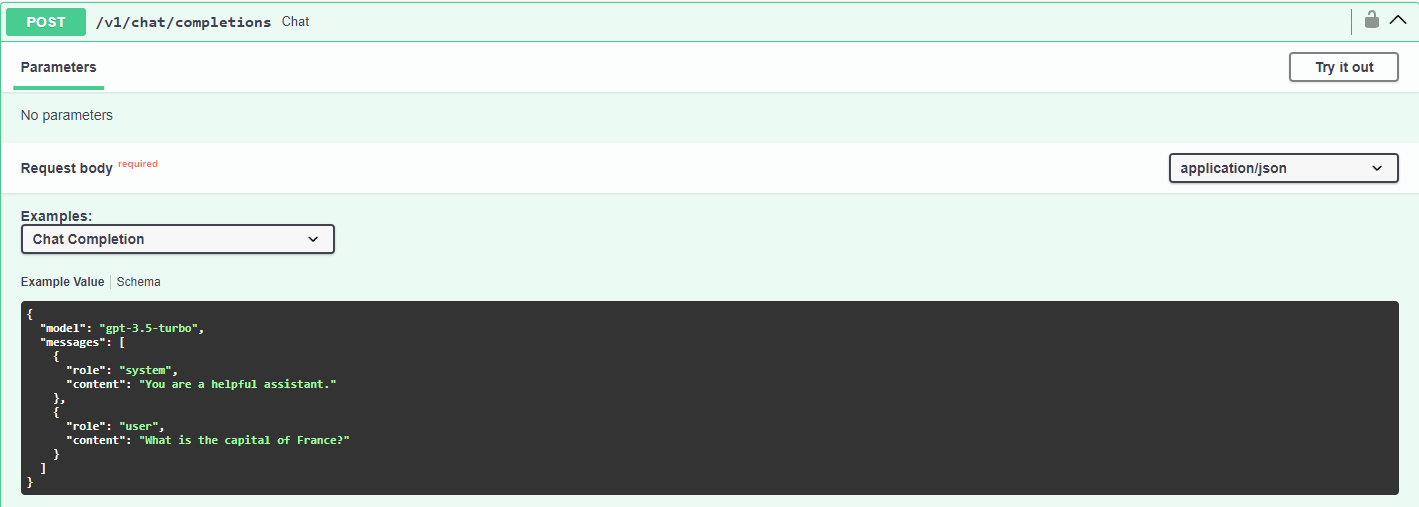
\includegraphics[width=1.0\textwidth]{figures/figure_2_16.png}
% \\
% \parbox[t]{\textwidth}{\vspace{1ex}\large\hspace*{7.5mm}}
\captionsetup{style=figureStyle}
\caption{Endpoint /v1/chat/completions with POST method to generate question answering records}\label{fig.2.16}
\end{figure}

\begin{figure}[h]
\centering
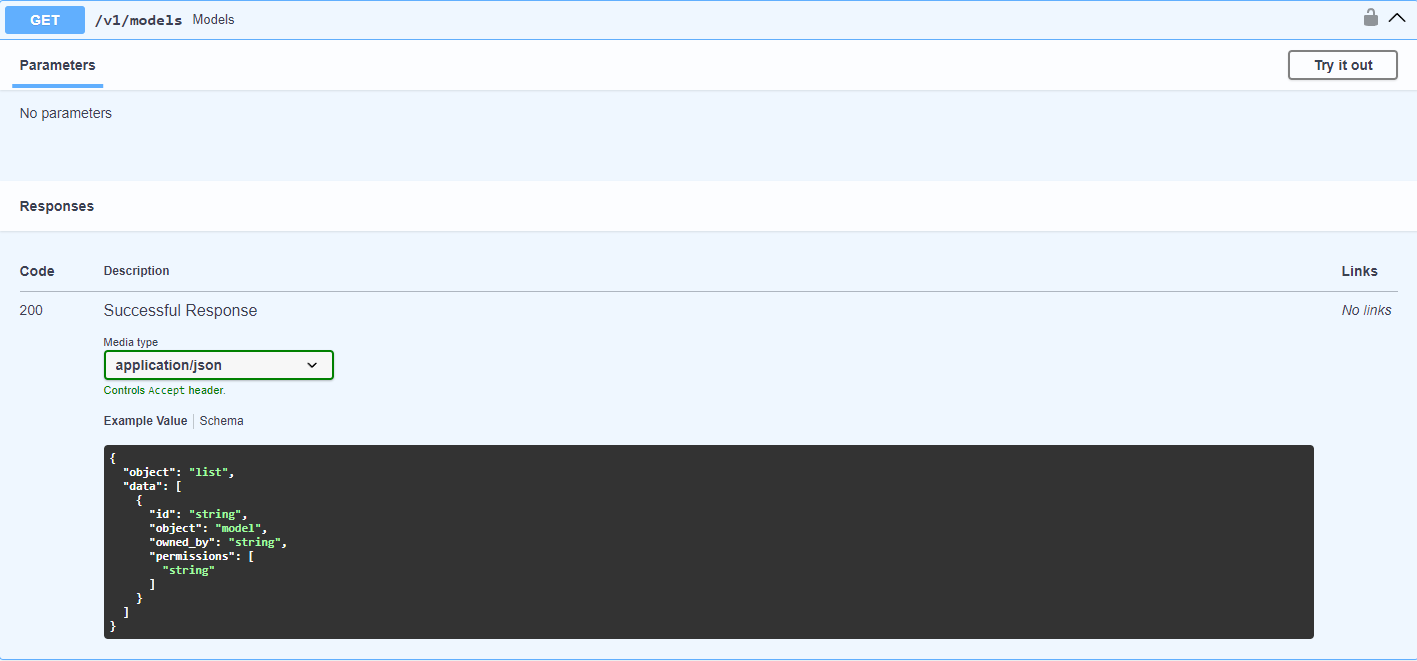
\includegraphics[width=1.0\textwidth]{figures/figure_2_17.png}
% \\
% \parbox[t]{\textwidth}{\vspace{1ex}\large\hspace*{7.5mm}}
\captionsetup{style=figureStyle}
\caption{Endpoint /v1/models with GET method to list all available models}\label{fig.2.17}
\end{figure}

Additionally, it was decided to implement the RAG (Retrieval-Augmented Generation) pipeline. This involves extracting part of the context from the database as a prompt for the model to generate responses based on the database, which serves as an alternative to fine-tuning and does not require retraining the model or additional costs. Retrieving relevant documents is facilitated by the interaction between the Langchain framework and Sentence-Transformers library, which provide a wrapper for the embedding model that ranks texts based on their similarity using cosine similarity metric. Based on metrics from the MTEB leaderboard on the Hugging Face platform, the decision was made to utilize the bge-m3 model for generating and searching embeddings. The complete schema of the RAG pipeline is represented in figure 2.18.

\begin{figure}[h]
\centering
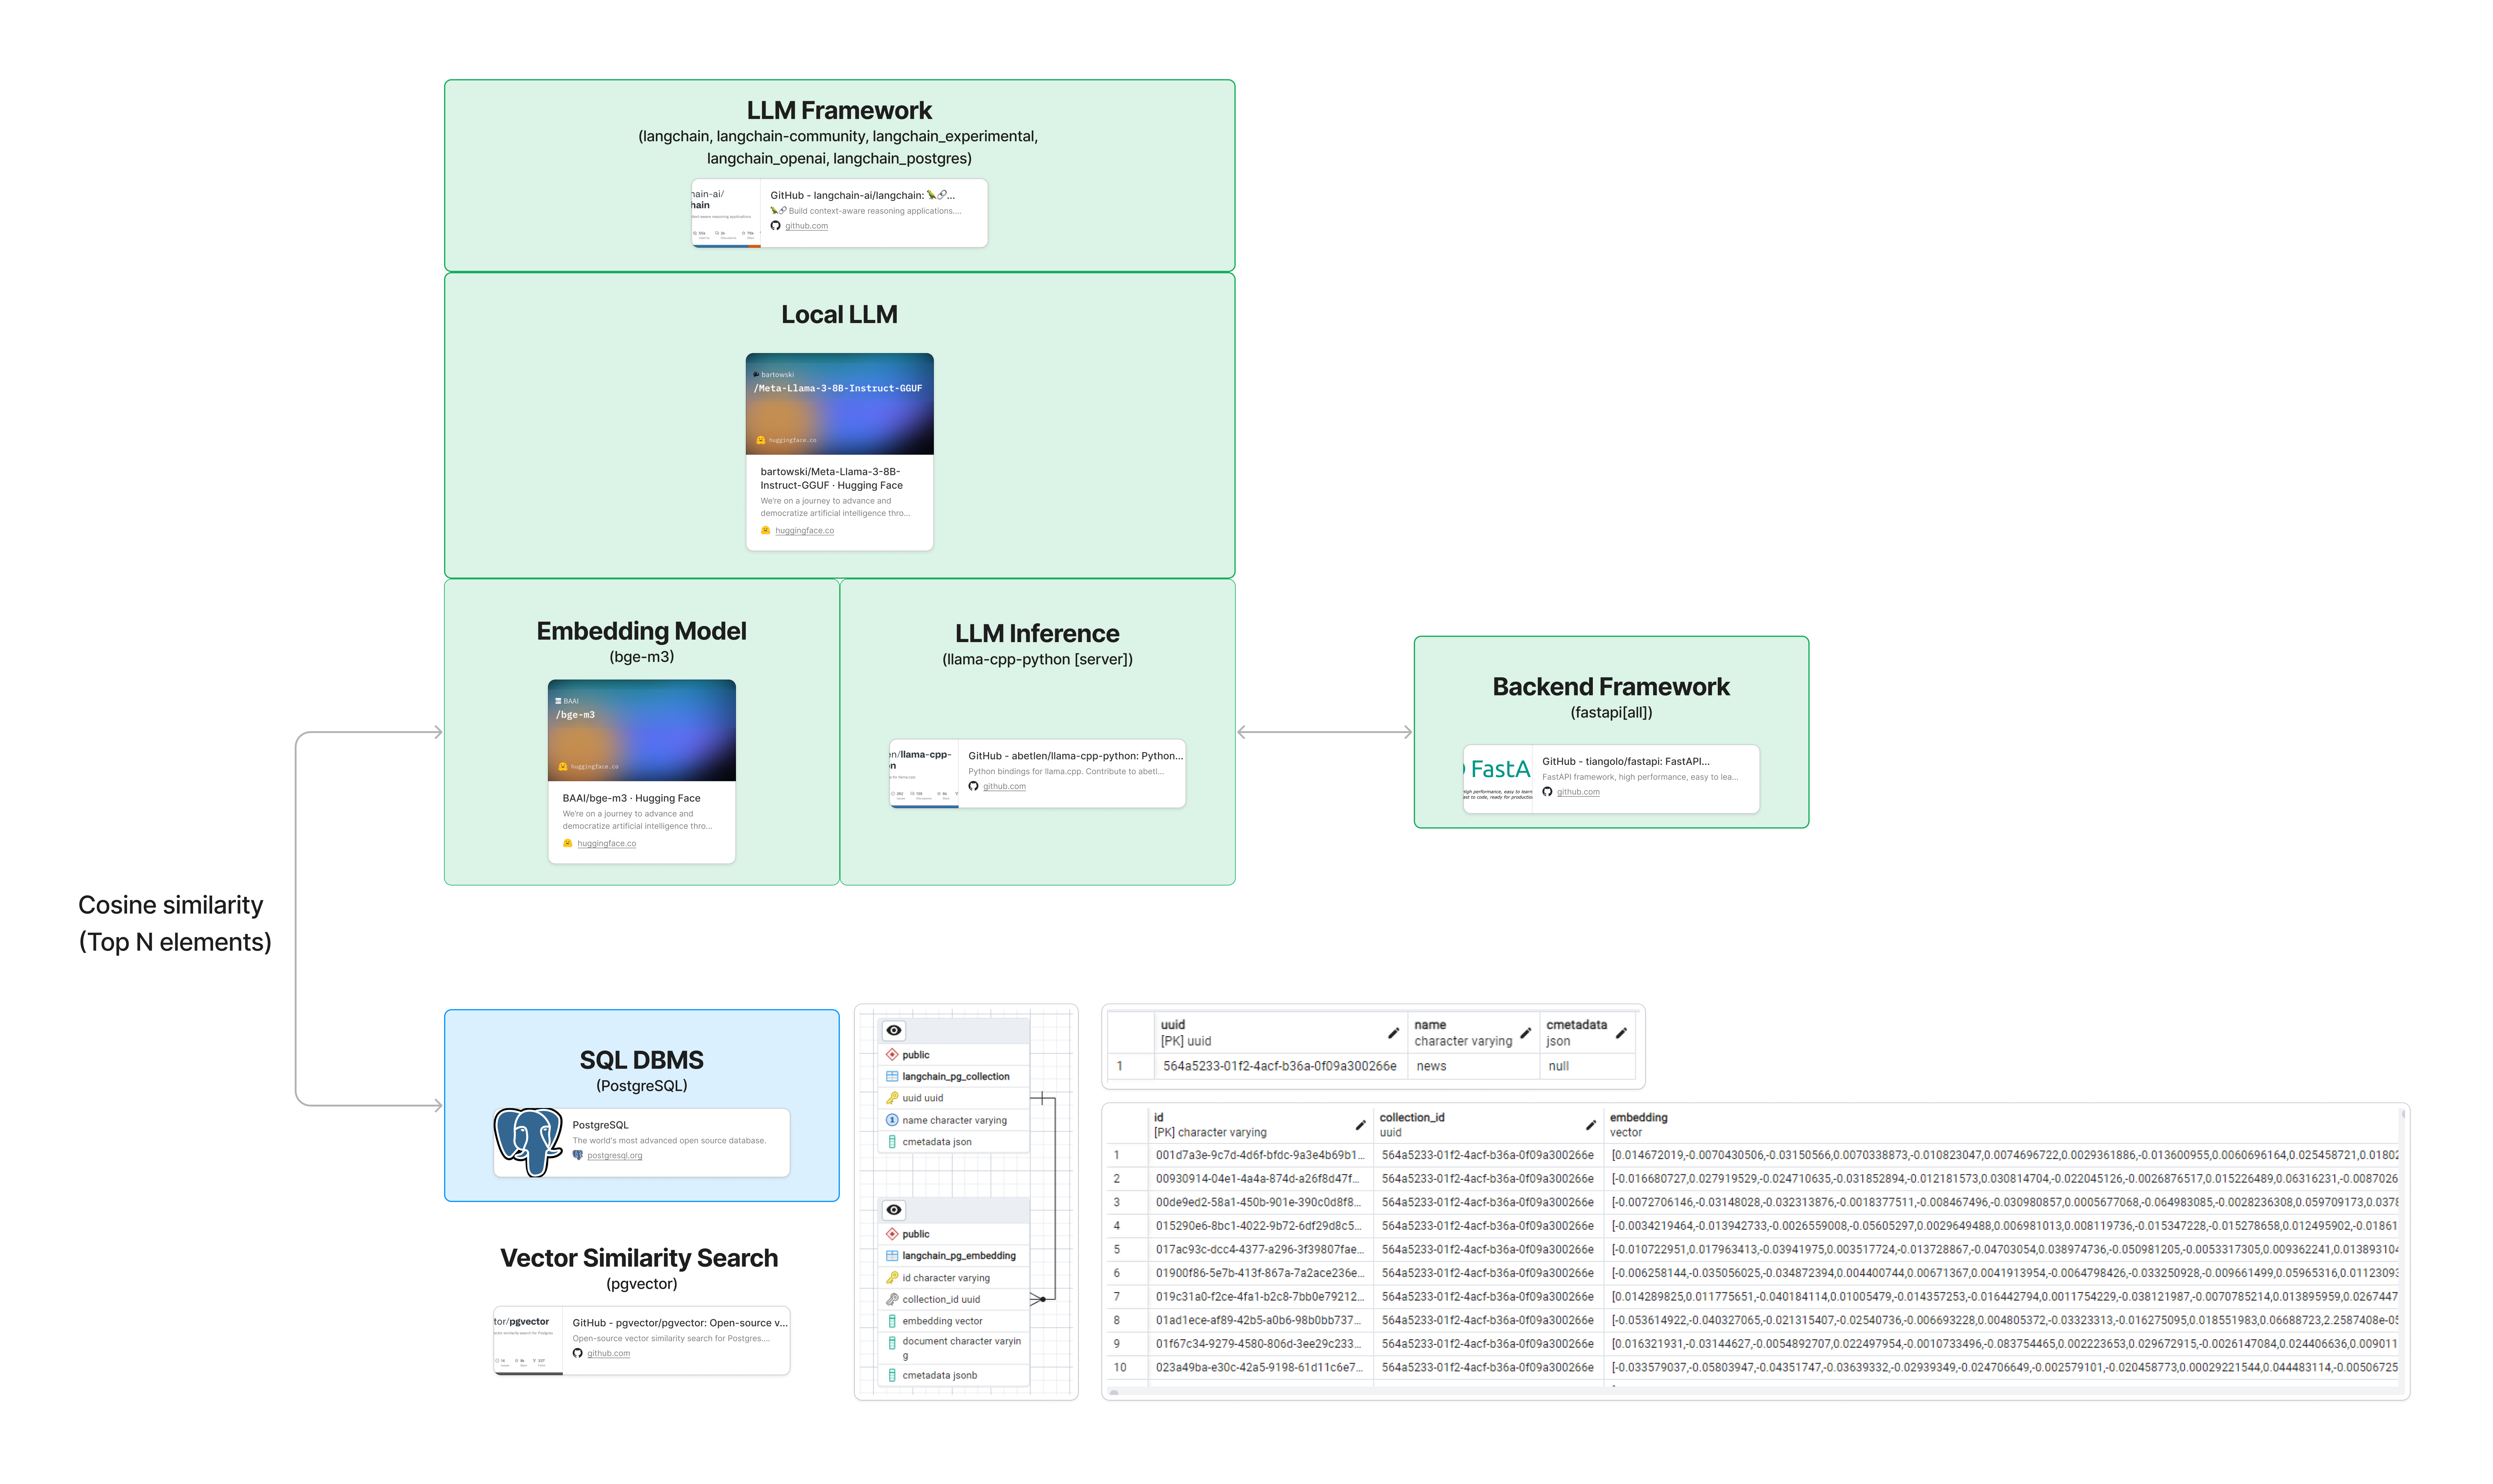
\includegraphics[width=1.0\textwidth]{figures/figure_2_18.png}
% \\
% \parbox[t]{\textwidth}{\vspace{1ex}\large\hspace*{7.5mm}}
\captionsetup{style=figureStyle}
\caption{A basic RAG pipeline}\label{fig.2.18}
\end{figure}

The open-source tool Langfuse was also applied for monitoring and tracing the underlying operations of the LLM and Langchain. All this information is showcased in figures 2.19, 2.20, 2.21, 2.22, 2.23, 2.24, 2.25, and 2.26.

\begin{figure}[h]
\centering
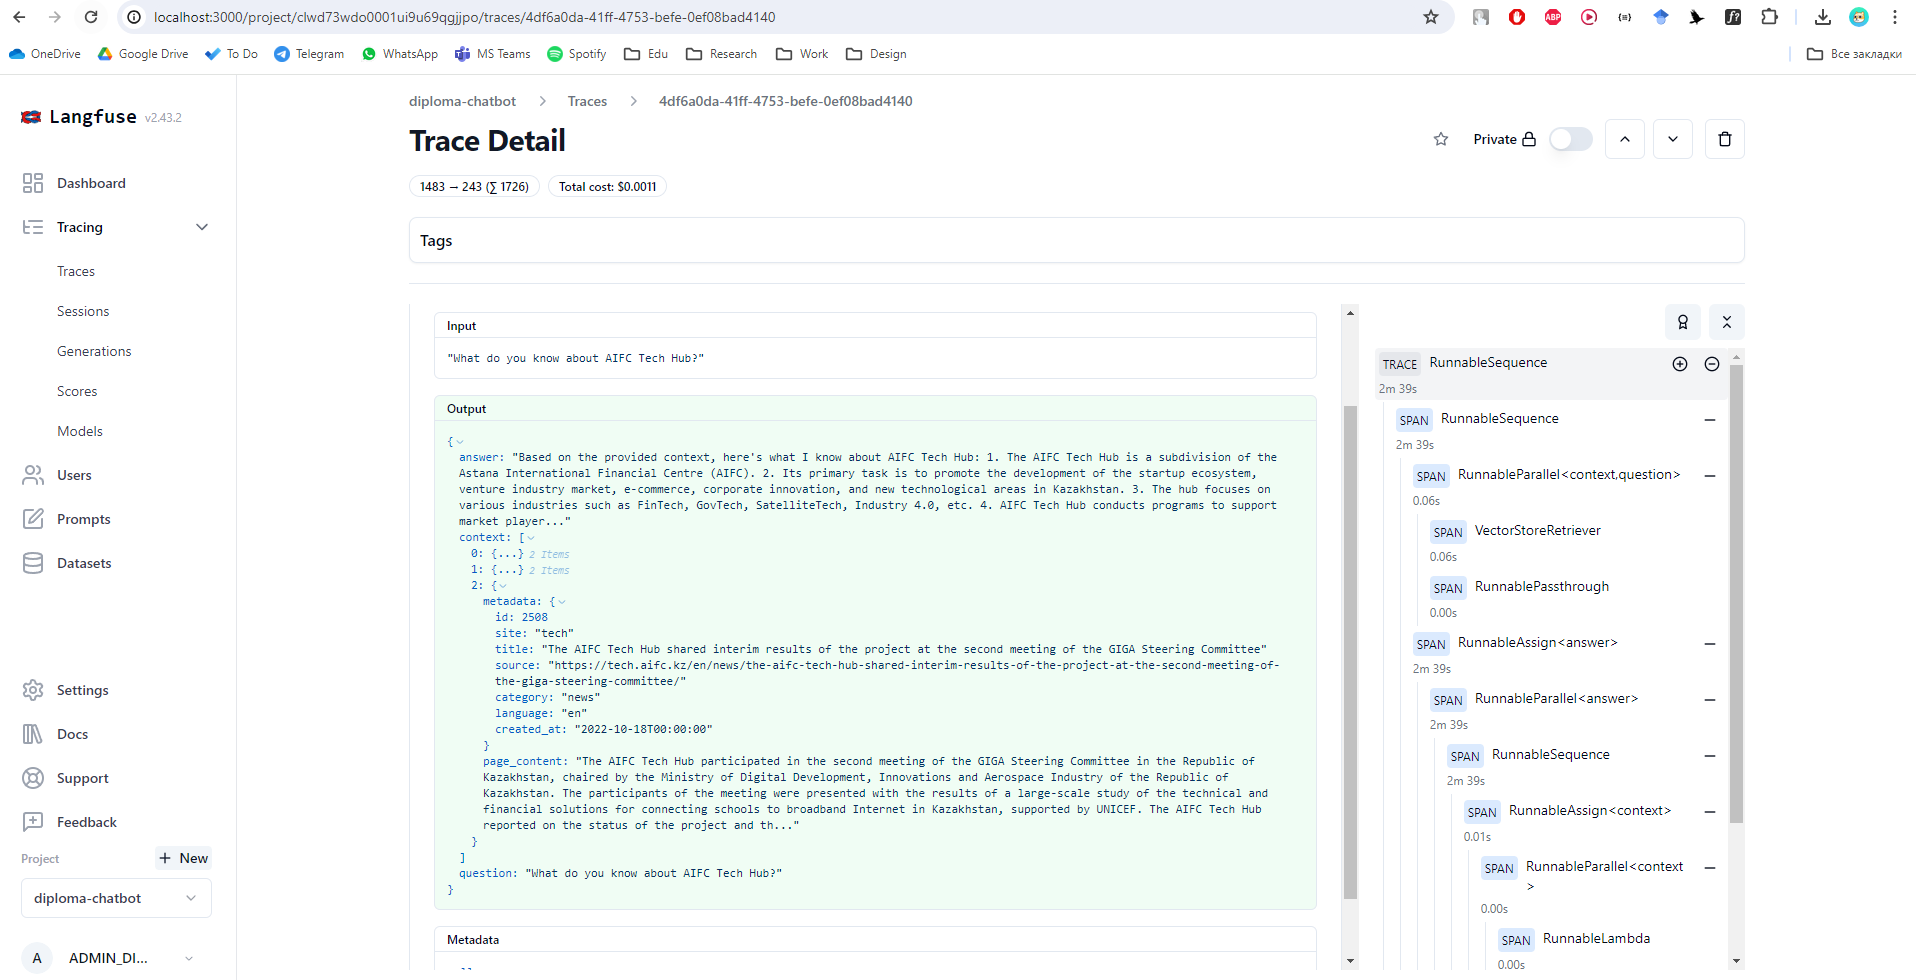
\includegraphics[width=0.7\textwidth]{figures/figure_2_19.png}
% \\
% \parbox[t]{\textwidth}{\vspace{1ex}\large\hspace*{7.5mm}}
\captionsetup{style=figureStyle}
\caption{Langfuse example with user question and retrieved documents from the database}\label{fig.2.19}
\end{figure}

\begin{figure}[h]
\centering
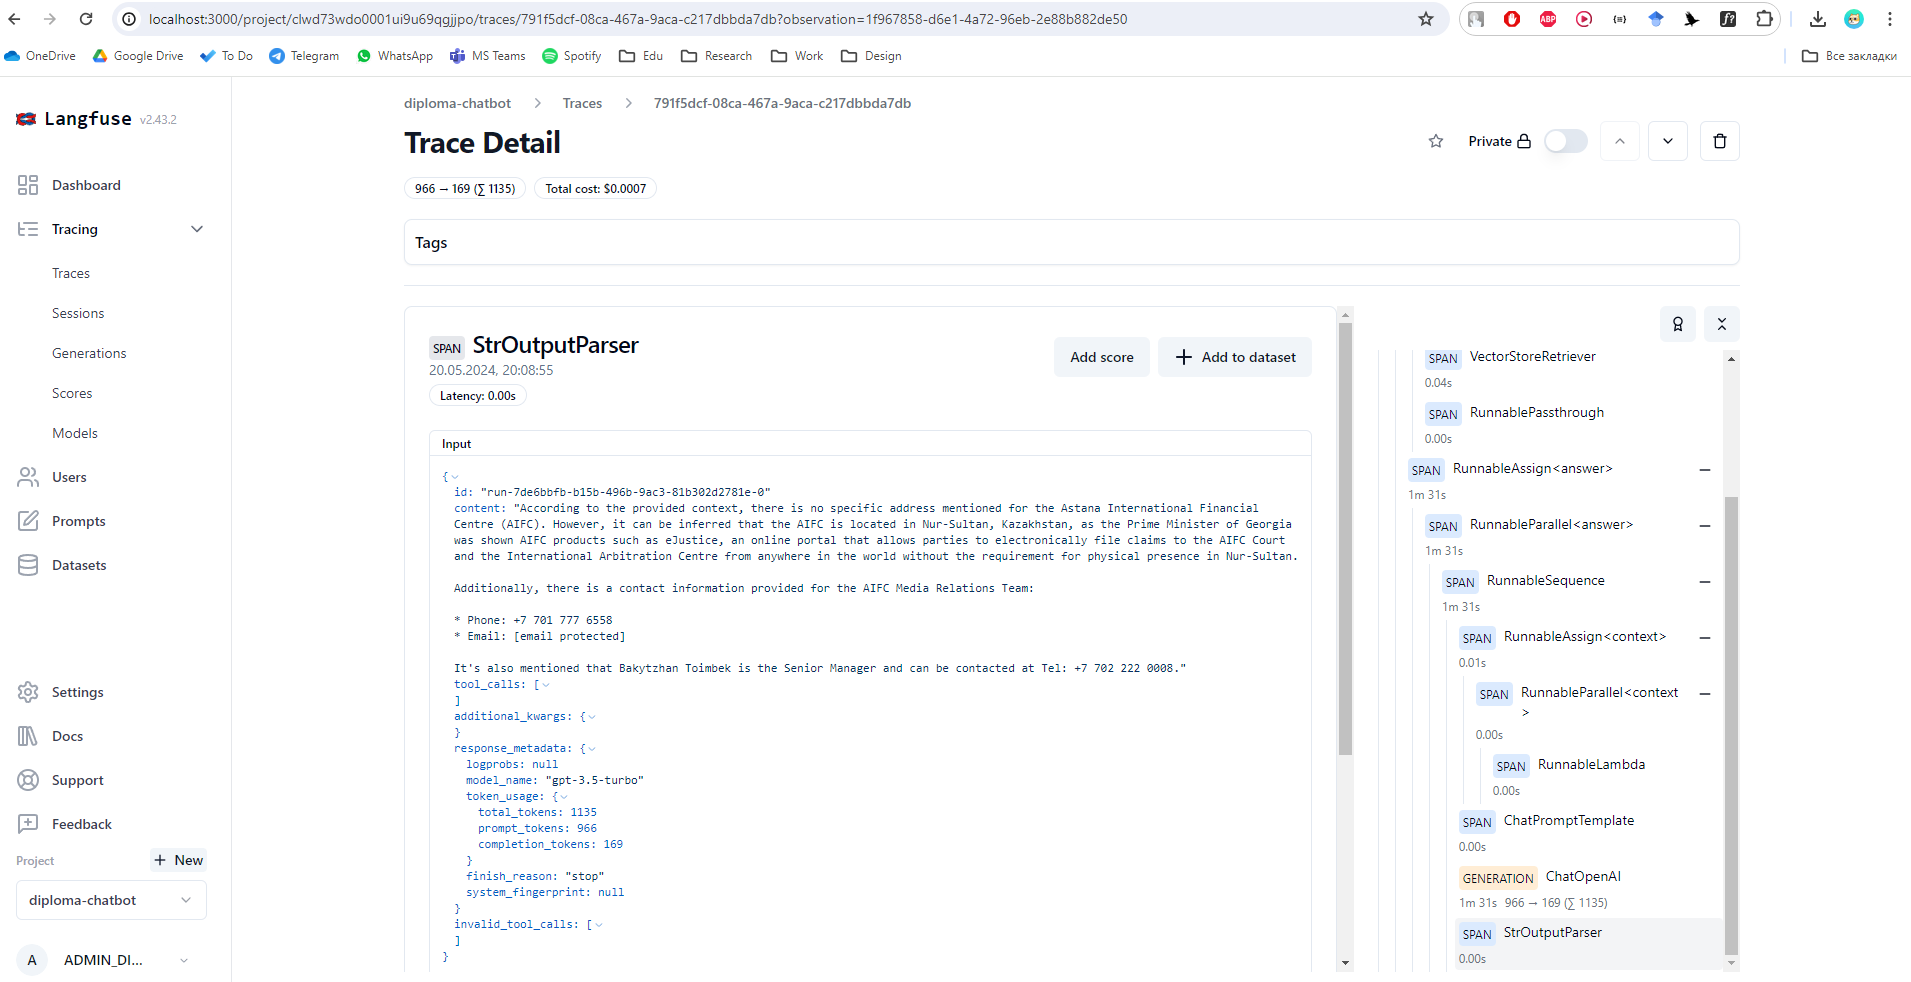
\includegraphics[width=1.0\textwidth]{figures/figure_2_20.png}
% \\
% \parbox[t]{\textwidth}{\vspace{1ex}\large\hspace*{7.5mm}}
\captionsetup{style=figureStyle}
\caption{Langfuse example with LLM-generated output}\label{fig.2.20}
\end{figure}

\begin{figure}[h]
\centering
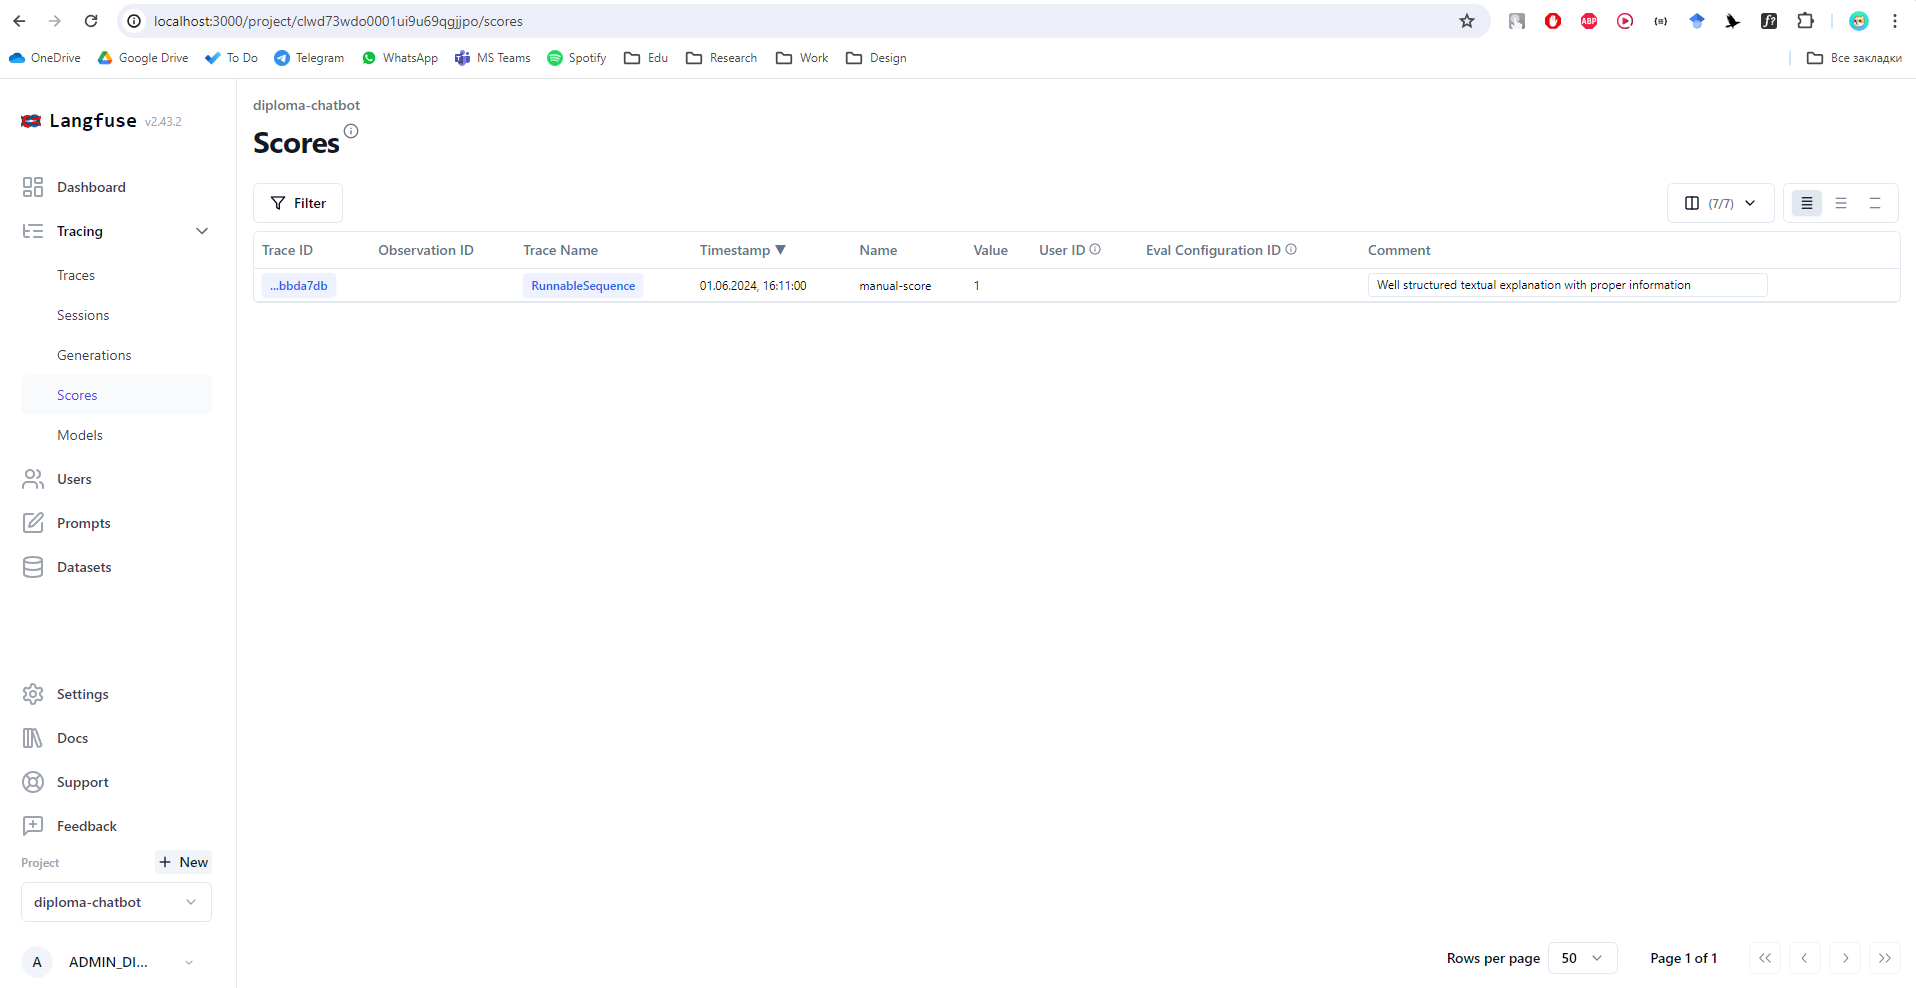
\includegraphics[width=1.0\textwidth]{figures/figure_2_21.png}
% \\
% \parbox[t]{\textwidth}{\vspace{1ex}\large\hspace*{7.5mm}}
\captionsetup{style=figureStyle}
\caption{Langfuse example of traceback scoring}\label{fig.2.21}
\end{figure}

\begin{figure}[h]
\centering
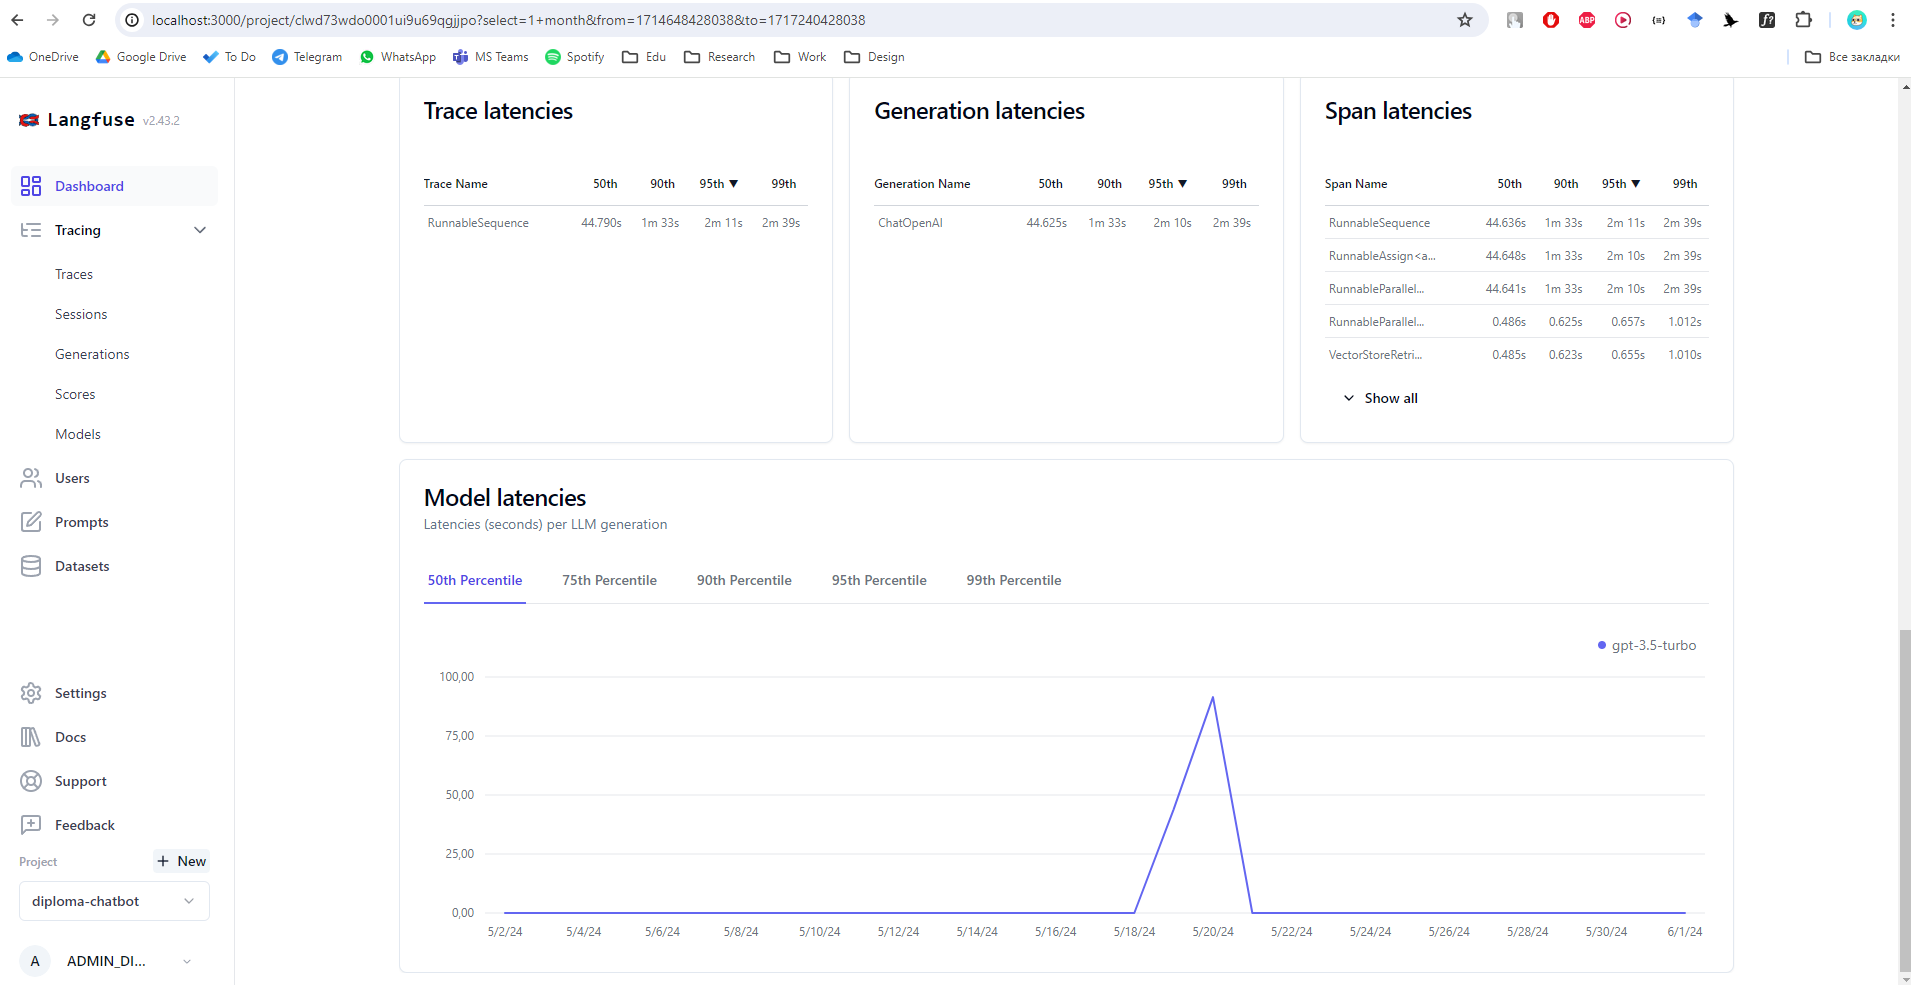
\includegraphics[width=1.0\textwidth]{figures/figure_2_22.png}
% \\
% \parbox[t]{\textwidth}{\vspace{1ex}\large\hspace*{7.5mm}}
\captionsetup{style=figureStyle}
\caption{Langfuse example with latency tracebacks}\label{fig.2.22}
\end{figure}

\begin{figure}[h]
\centering
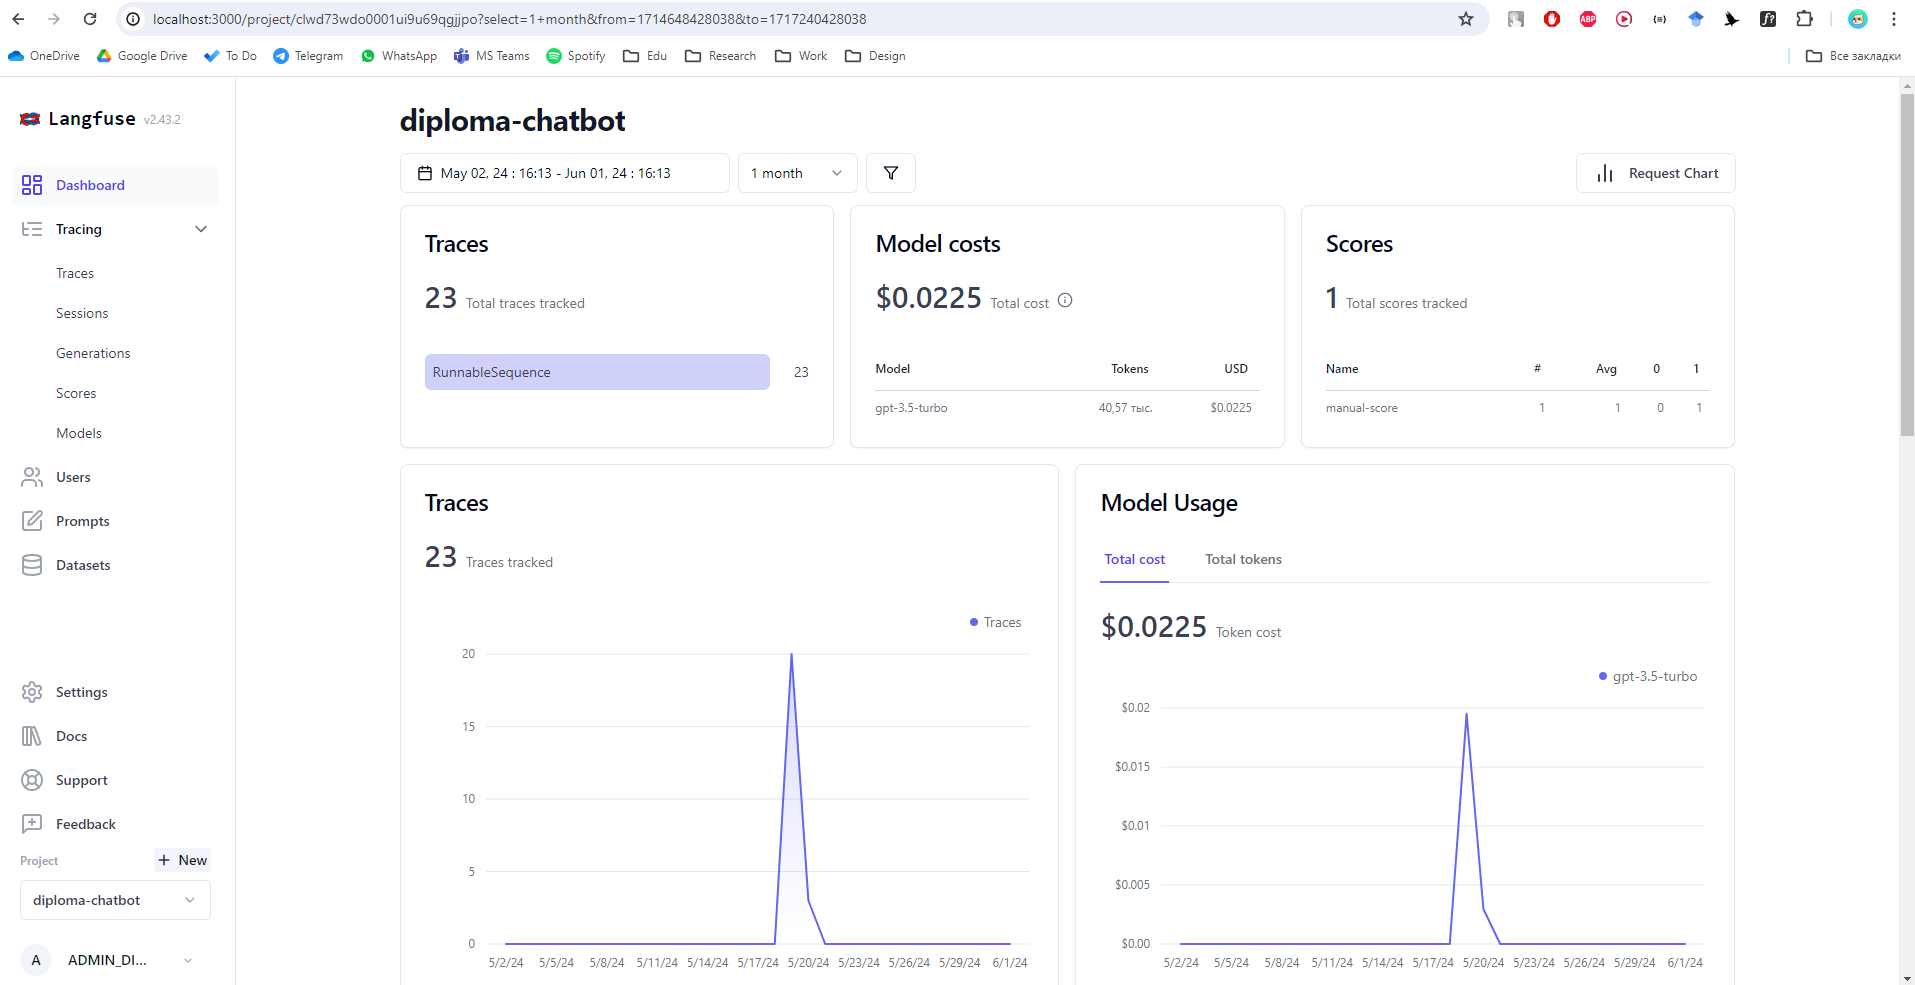
\includegraphics[width=1.0\textwidth]{figures/figure_2_23.png}
% \\
% \parbox[t]{\textwidth}{\vspace{1ex}\large\hspace*{7.5mm}}
\captionsetup{style=figureStyle}
\caption{Langfuse example with price tracebacks}\label{fig.2.23}
\end{figure}

\begin{figure}[h]
\centering
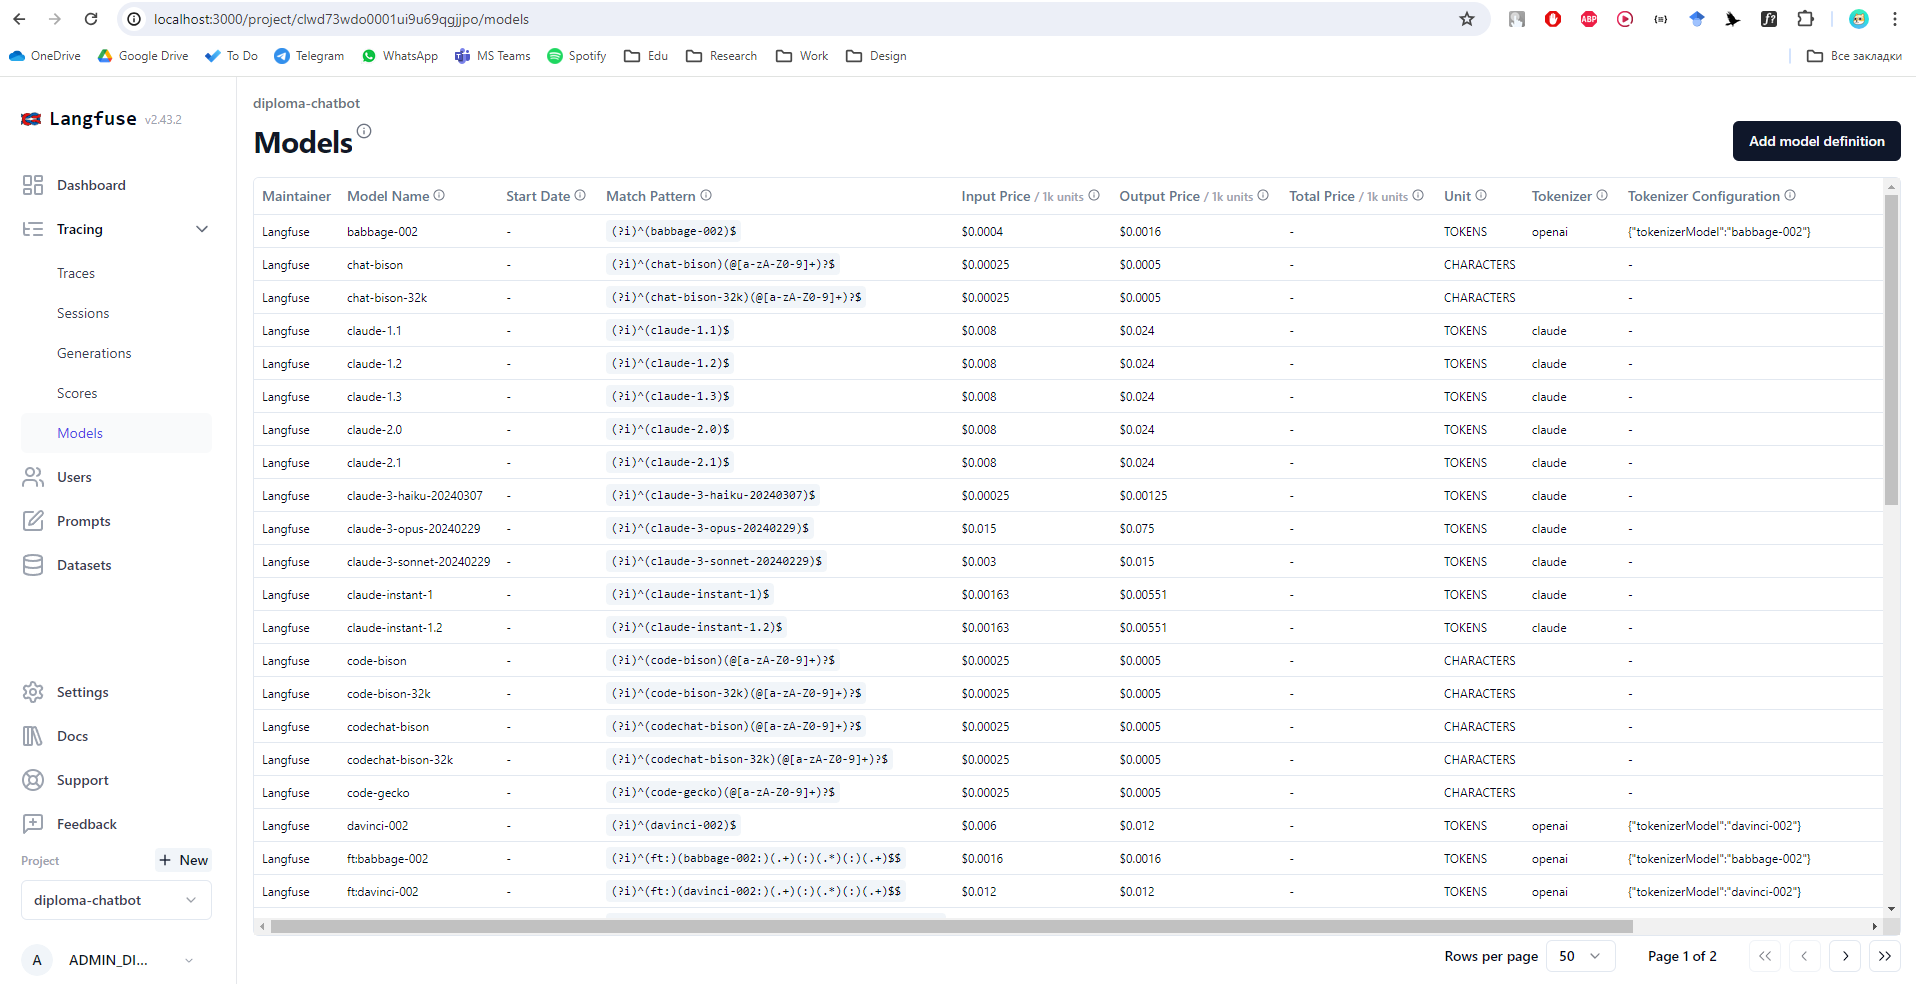
\includegraphics[width=1.0\textwidth]{figures/figure_2_24.png}
% \\
% \parbox[t]{\textwidth}{\vspace{1ex}\large\hspace*{7.5mm}}
\captionsetup{style=figureStyle}
\caption{Langfuse example with model-based price calculations}\label{fig.2.24}
\end{figure}

\begin{figure}[h]
\centering
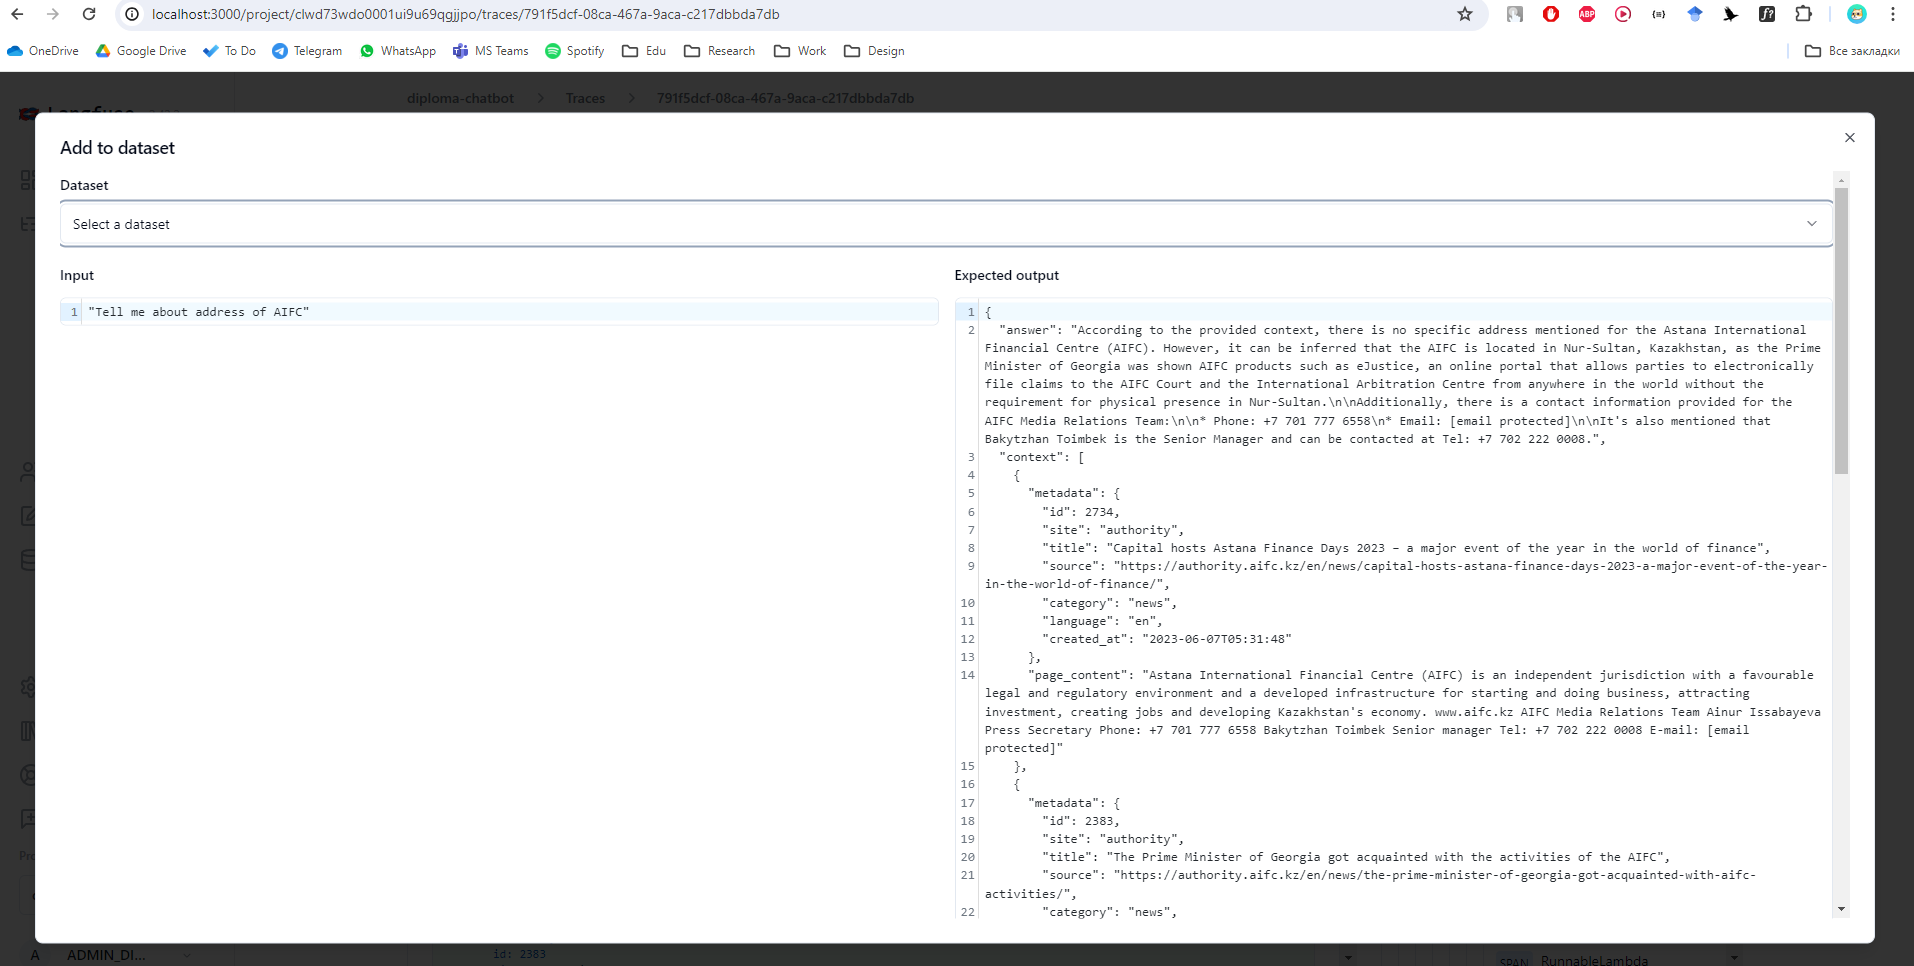
\includegraphics[width=1.0\textwidth]{figures/figure_2_25.png}
% \\
% \parbox[t]{\textwidth}{\vspace{1ex}\large\hspace*{7.5mm}}
\captionsetup{style=figureStyle}
\caption{Langfuse example for generating datasets from tracebacks}\label{fig.2.25}
\end{figure}

\begin{figure}[h]
\centering
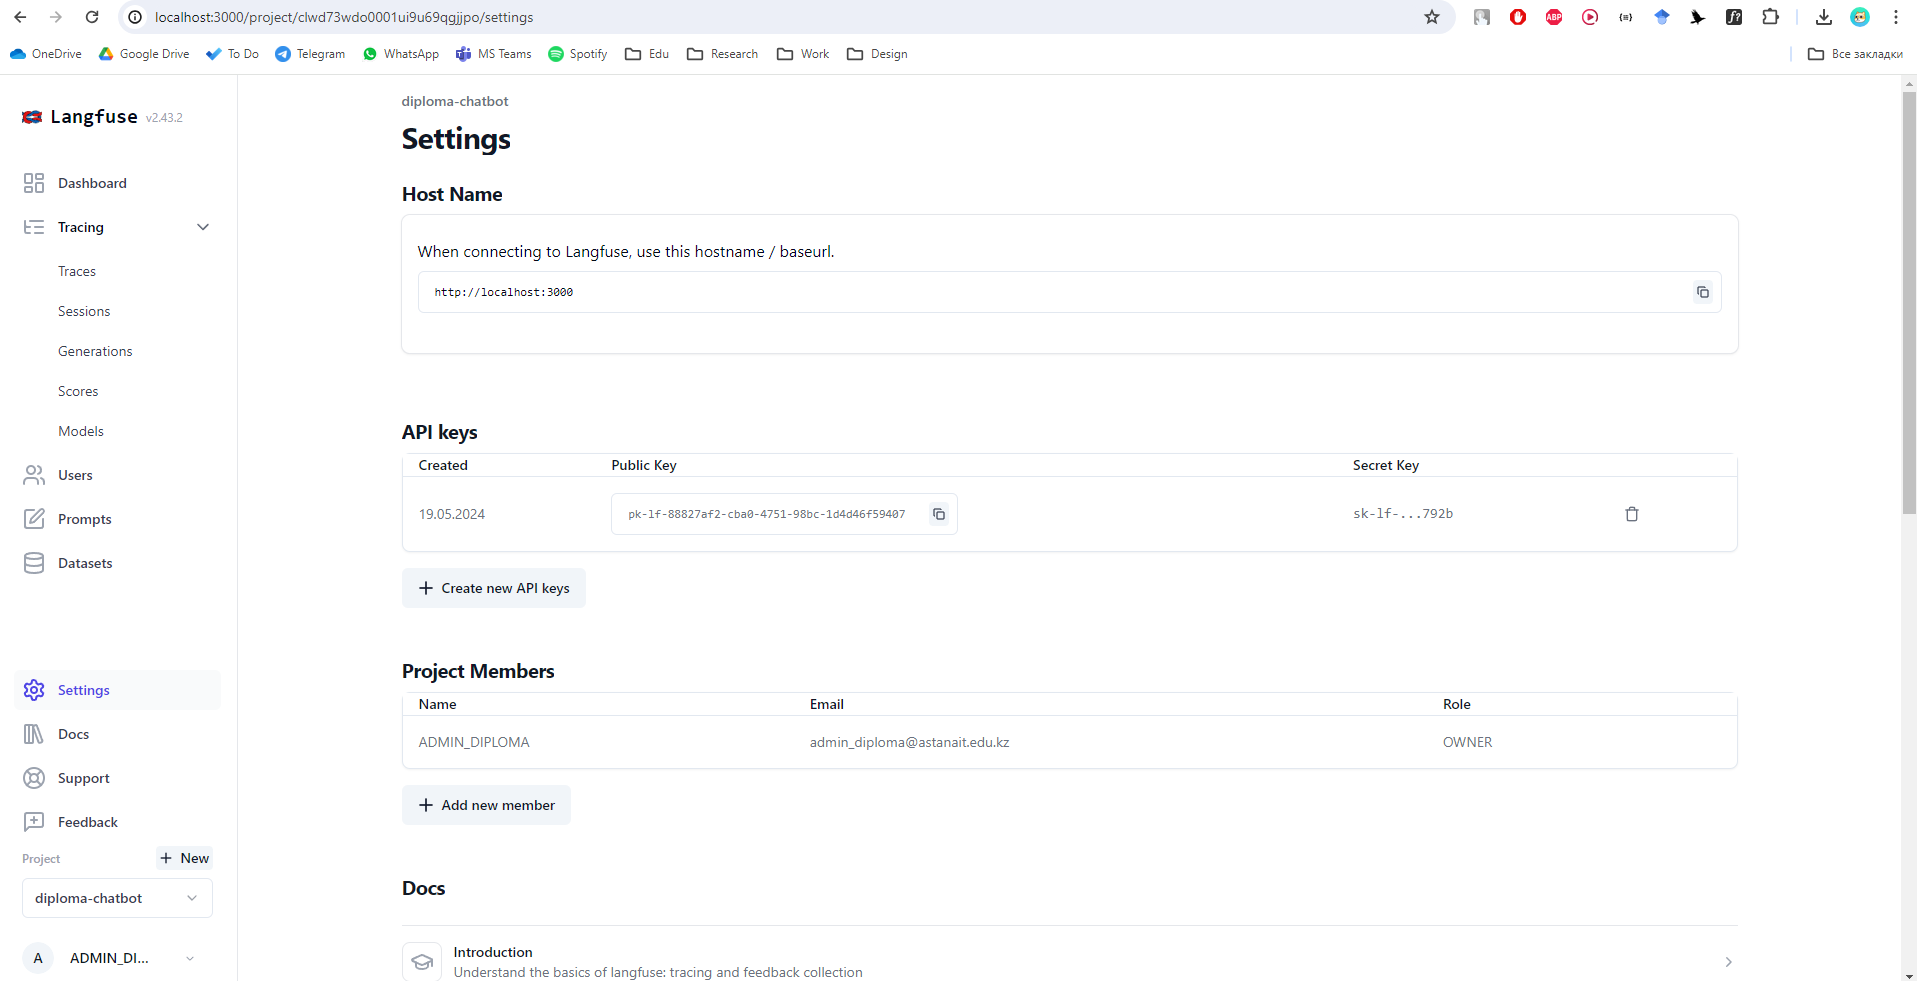
\includegraphics[width=1.0\textwidth]{figures/figure_2_26.png}
% \\
% \parbox[t]{\textwidth}{\vspace{1ex}\large\hspace*{7.5mm}}
\captionsetup{style=figureStyle}
\caption{Langfuse example for API keys configuration}\label{fig.2.26}
\end{figure}

Containerization was utilized for hosting Langfuse and the database. This approach addresses the issue of specific dependencies not being installed on a particular server or multiple applications conflicting with each other. Containers operate independently in isolation from certain system processes. Docker, along with its Compose specification, was applied for containerization.

% \section[Deployment]{Deployment}
% объяснить про деплоймент теорию. немного и сразу же показать что будет деплоитьмя в докере и пояснить за докер
% тут немного про ngrok рассказаь мб
% времени на nginx не будет поэтому про него только в результатах рассказать
% Appendix D, Docker Containerization, Deployment, Hosting

\clearpage

\section[Frontend service]{Frontend service}
\subsection{Comparison of frontend tools}
% объяснение позиции фронтенда в клиент серверной архитектуре и как обычно его делают (через реакт или любые другие js фреймворки)
The interaction between the frontend and backend is an integral component of any web application or platform. Usually, this process is implemented via API calls from the frontend to the backend using different HTTP methods. Especially when the frontend receives a response with a status code and objects in the form of JSON. Most frontends are written in JavaScript using the language itself, fetch wrappers given by frameworks, or specialized libraries like Axios.

% ситуация когда у вас только бэкендеры или вообще нету фронтендеров, то тогда надо использовать альтернативы для быстрого фронтенда (jinja templates, gradio, streamlit) - но нужно упомянуть что это временное решение и трудномасштабируемое
However, there are situations where a team lacks frontend developers or similar roles. In such cases, alternative approaches can be utilized, such as:

- Jinja2 templates is based on HTML, it allows for the integrations of complex functionality. These HTML pages can be directly returned as ``TemplateResponse'' or ``HTMLResponse'' from the FastAPI backend.

- Gradio and streamlit libraries enable frontend development via Python language. There are based on the React frontend library and offer pre-made components with state management. On the other hand, streamlit is more frexible with support of custom components creation. 

- Low-code solutions or other alternative methodologies, which are included in many low-code platforms, can also be evaluated for frontend development.

However, it is critical to note that some solutions may not be appropriate or easily scalable for large companies. The choice of frontend development tools should be based on what is popular and supported within a specific workplace.

% описание архитектуры, принцип работы, показ визуальных частей
% объяснение что такое стримлит что под капотом там реакт компоненты но они ререглеряться и про состояния потом объяснить про структуру фронтеда и визуальные его части как дергает апи
\subsection{General overview and explanation of frontend part}
As a result, for this project, it was decided to use the Streamlit library due to its numerous advantages and features mentioned above. All the main code snippets are provided in Appendix C. Firstly, main.py serves as the central file, initially checking for the presence of a JWT token in the browser cookies. If the token is absent, it redirects to a page with a login and registration form, as demonstrated in figures 2.27 and 2.28.

\begin{figure}[h]
\centering
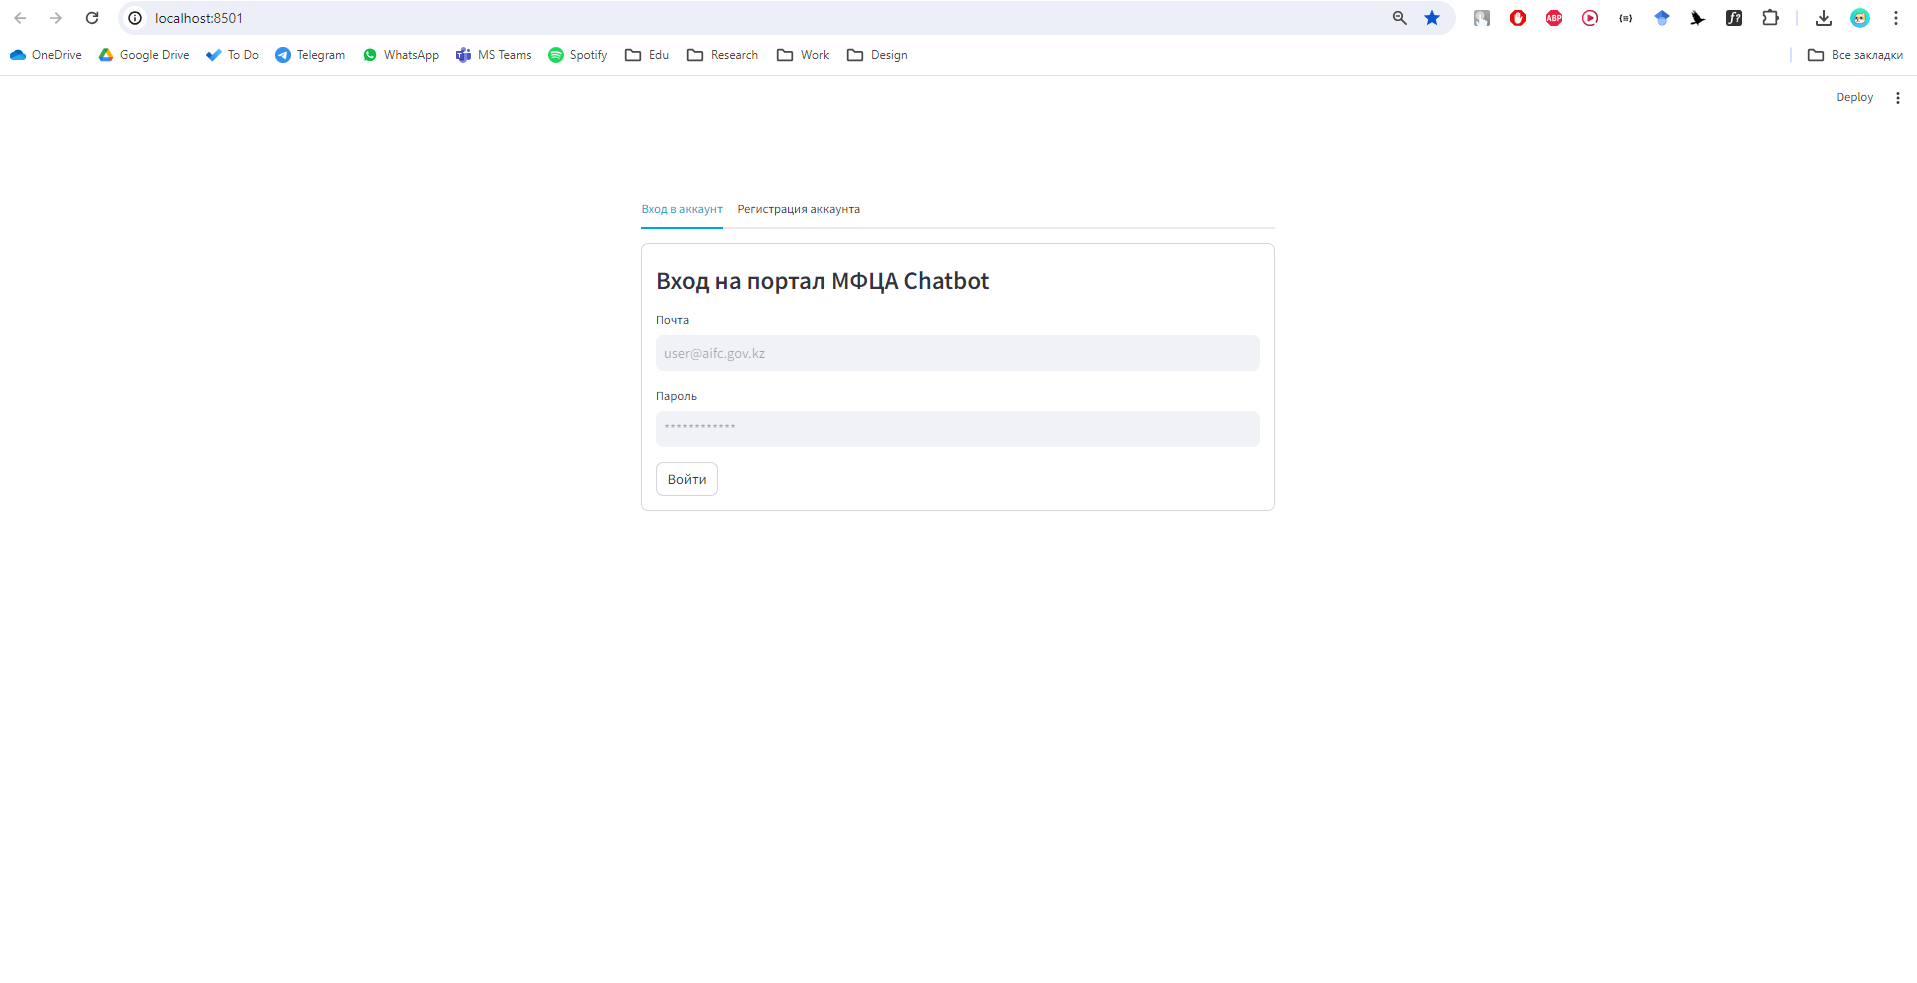
\includegraphics[width=0.55\textwidth]{figures/figure_2_27.png}
% \\
% \parbox[t]{\textwidth}{\vspace{1ex}\large\hspace*{7.5mm}}
\captionsetup{style=figureStyle}
\caption{Login form}\label{fig.2.27}
\end{figure}

\begin{figure}[h]
\centering
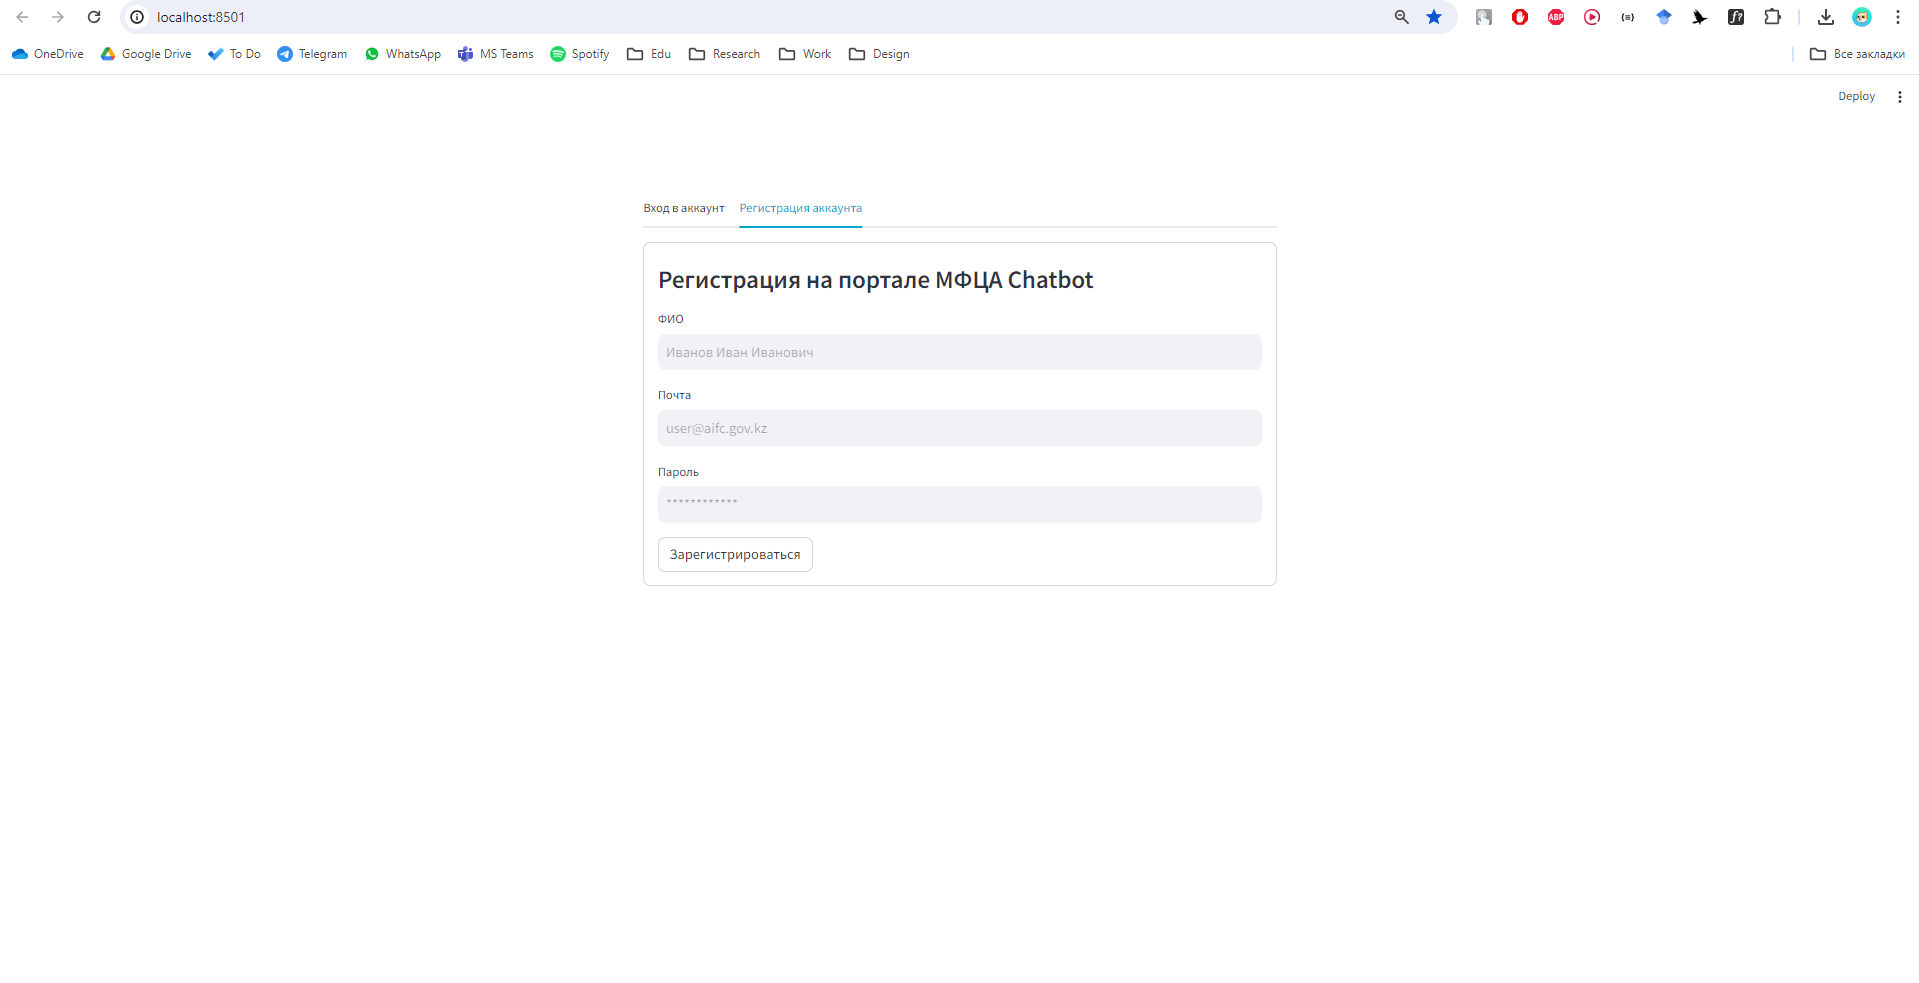
\includegraphics[width=1.0\textwidth]{figures/figure_2_28.png}
% \\
% \parbox[t]{\textwidth}{\vspace{1ex}\large\hspace*{7.5mm}}
\captionsetup{style=figureStyle}
\caption{Register form}\label{fig.2.28}
\end{figure}

Secondly, if the user successfully logs in or registers, the page will re-render and redirect to the chatbot page. This page presents several key elements, such as a sidebar panel and the chat window itself. In the sidebar panel, users can view their information, create a new chat, select a chat, and navigate through the chat list with pagination. Clicking on a chat UUID button opens the chat window, which includes several components, as displayed in figure 2.29: a dialogue panel with the bot and message history, a label indicating the current selected chat, an input panel for queries or messages, options for selecting data sources, language preferences for sources, and a brief note about the system.

\begin{figure}[h]
\centering
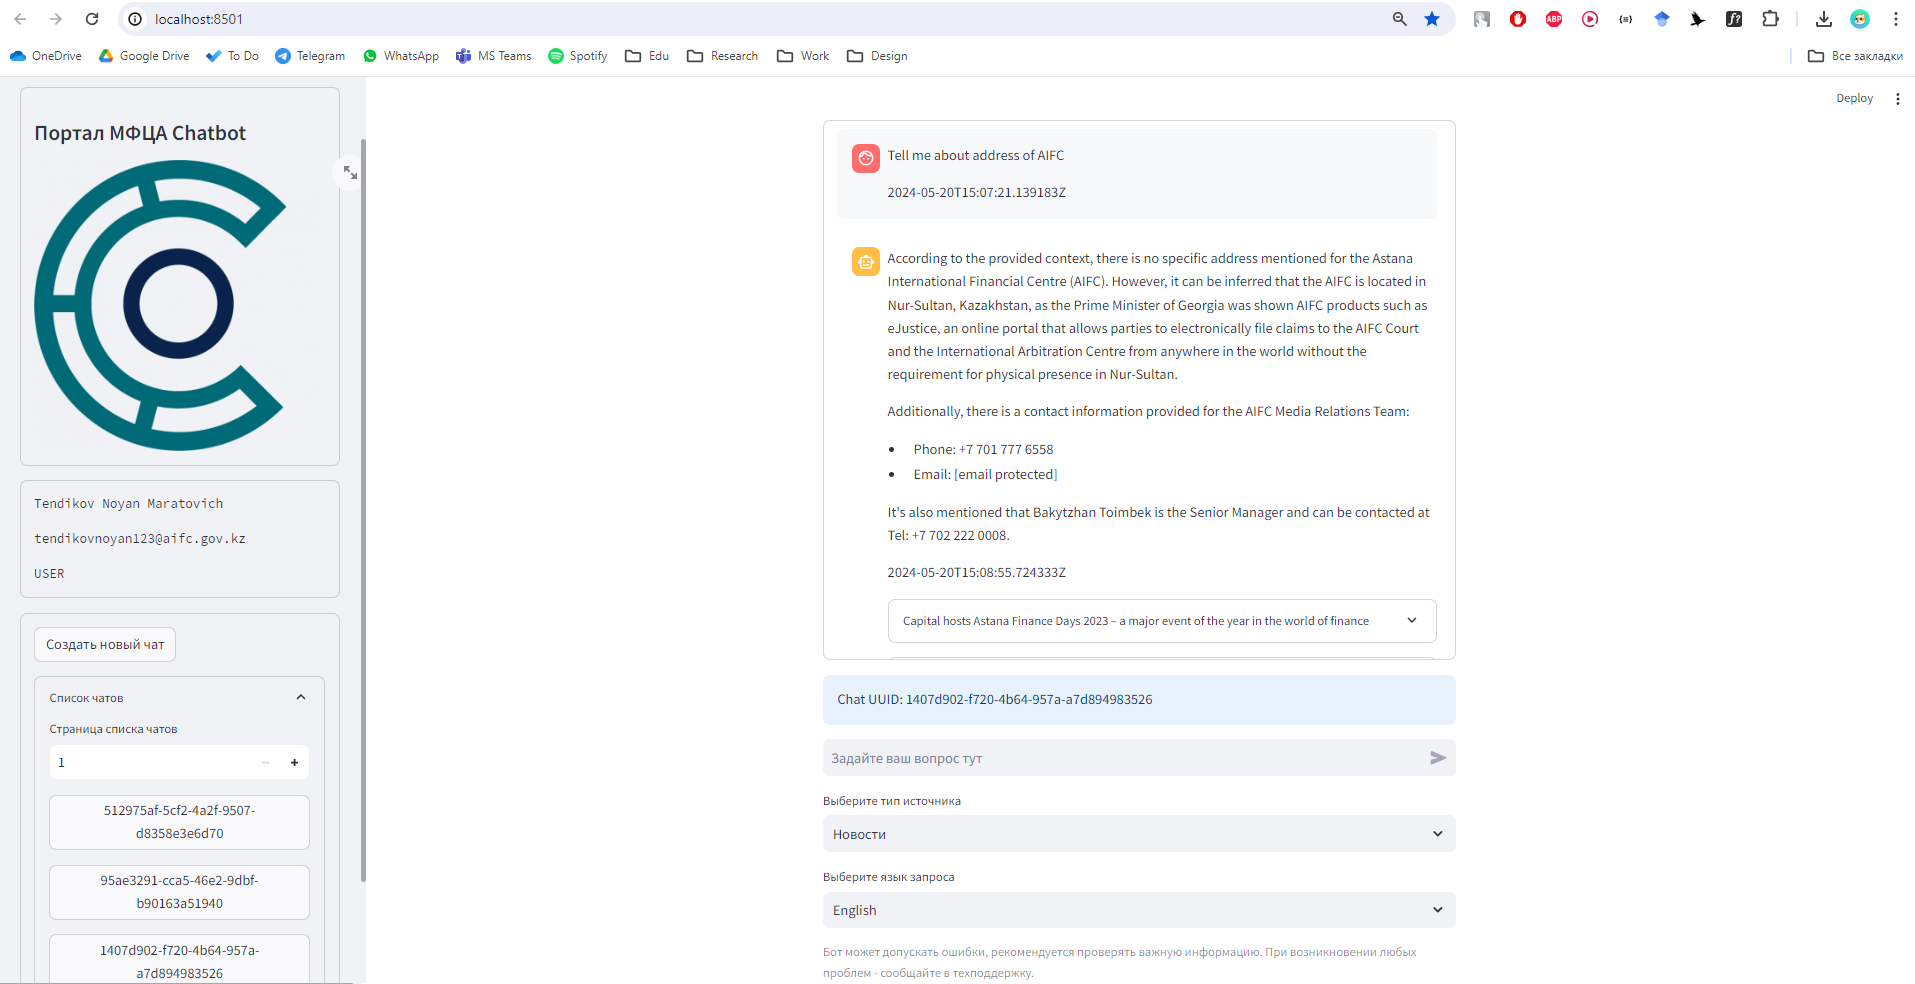
\includegraphics[width=0.8\textwidth]{figures/figure_2_29.png}
% \\
% \parbox[t]{\textwidth}{\vspace{1ex}\large\hspace*{7.5mm}}
\captionsetup{style=figureStyle}
\caption{Example of chatbot dialog}\label{fig.2.29}
\end{figure}

Thirdly, within the chat history with the bot, in addition to the standard responses to questions, several data sources used to formulate the response are displayed. Users can click on these sources to access more detailed information, as indicated in figure 2.30.

\begin{figure}[h]
\centering
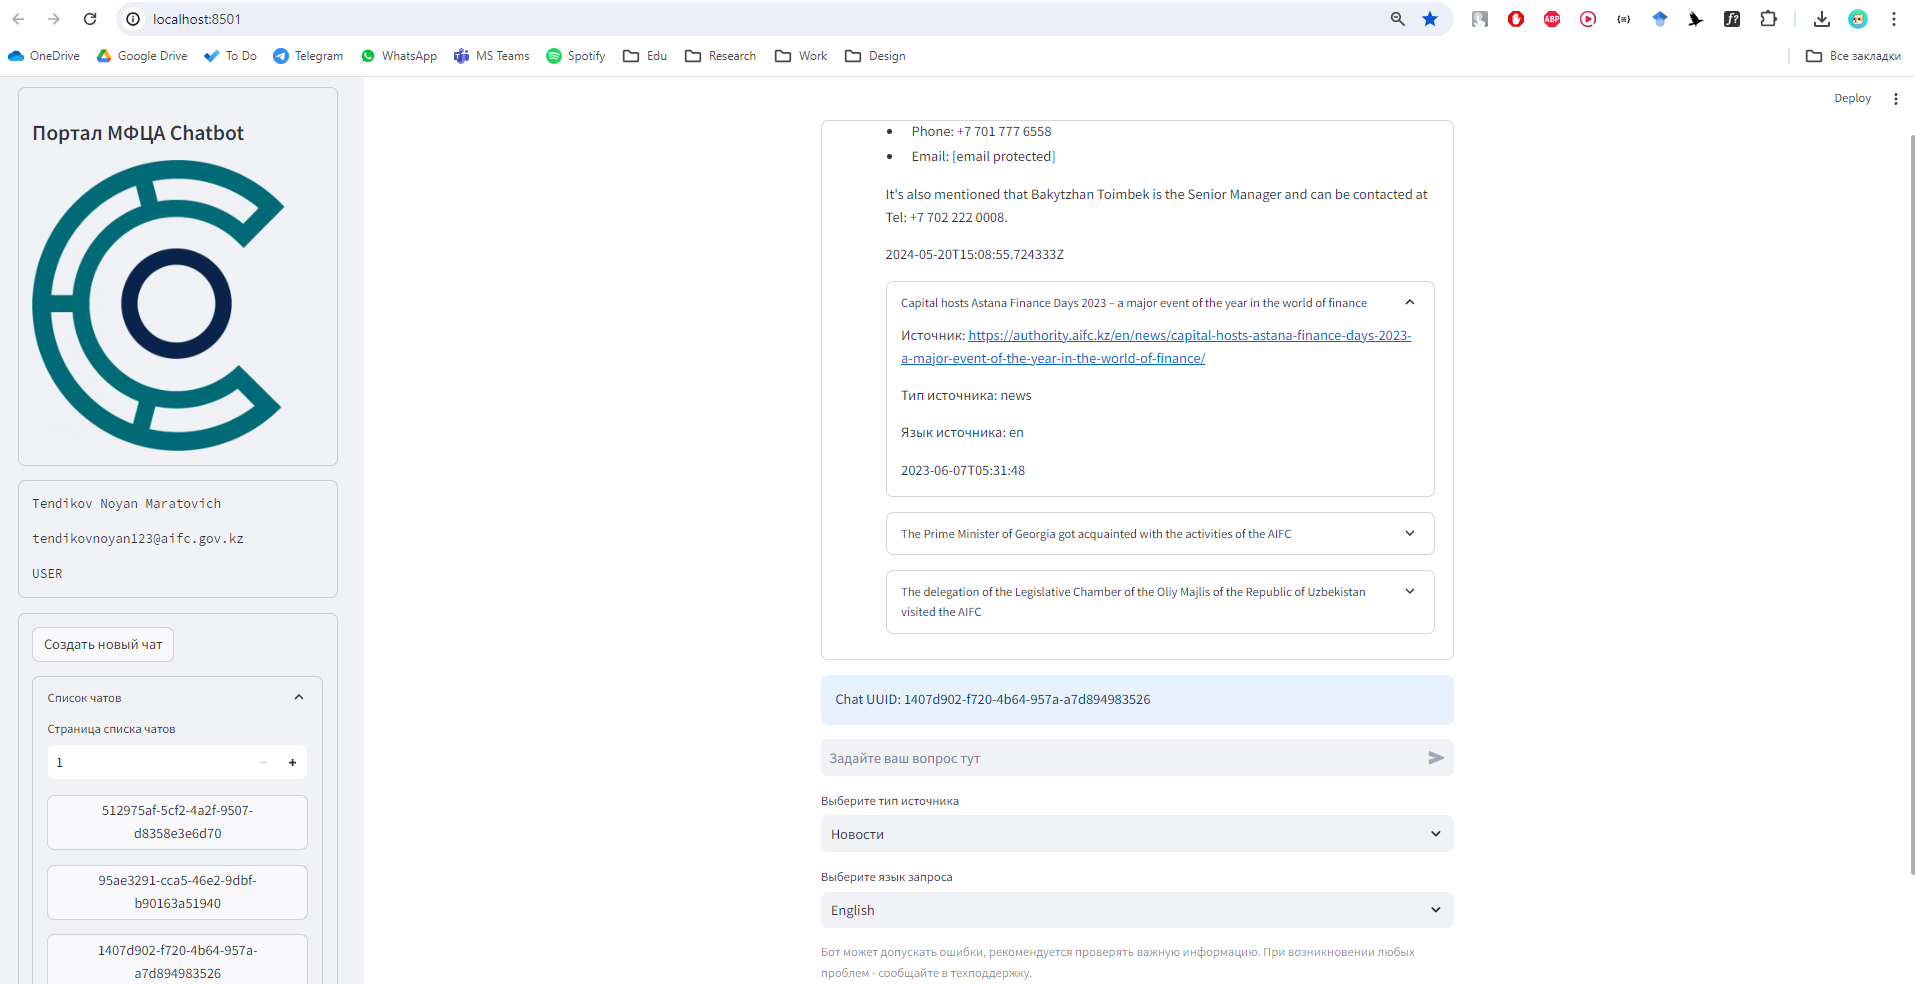
\includegraphics[width=1.0\textwidth]{figures/figure_2_30.png}
% \\
% \parbox[t]{\textwidth}{\vspace{1ex}\large\hspace*{7.5mm}}
\captionsetup{style=figureStyle}
\caption{Example of detailed information with sources}\label{fig.2.29}
\end{figure}

Lastly, the frontend part currently implements only the basic core functionality and does not aim to utilize all backend endpoints, due to the fact that certain endpoints are only administrative or insignificant.

\clearpage

\chapter*[Conclusion and results]{CONCLUSION}
% Небольшое общее вводное подведение итогов
% Сильные и слабые (downsides) стороны работы + оценить перспективы темы развития исследований
% Research and implement the MLOps methodology by organizing procedures of development, testing, deployment, hosting pipeline, and ensuring replicable workflow throughout the entire lifecycle of the product.
% \section[Theoretical part]{Theoretical part}
From a theoretical perspective, this thesis has explored and examined several aspects of the MLOps field. It has provided a comprehensive analysis of key concepts and methodologies within this domain:
\begin{itemize}
    %----------
    \item Determined that MLOps is an adjacent field that is either a part of DS or a direction within it, focusing on integrating DevOps paradigms into machine learning development processes.
    %----------
    \item Studied that MLOps provides a solution to the research replication crisis and aims at the practical implementation of various aspects.
    %----------
    \item Analyzed data pipeline processes and standards for data extraction and preparation as data-driven products.
    %----------
    \item Identified key aspects of improving team or company interactions through emphasizing clear methodologies and the step-by-step process of working with stakeholders.
    %----------
\end{itemize}

% Construct an API web service based on technological trends, architectural solutions, and security design methods.
% \section[Practical part]{Practical part}
The practical part was oriented on the developing a fully functional and secure web service based on MLOps principles. It incorporated best practices for automation, version control, and deployment, ensuring robust and scalable solutions:
\begin{itemize}
    %----------
    \item Implemented a compact pipeline for web scraping data from AIFC websites using the httpx and bs4 libraries.
    %----------
    \item The extracted data was loaded into a local PostgreSQL database with the PGVector addon, where it was stored as numerical values in a vector space as embeddings for search ranking.
    %----------
    \item Deployed a locally pre-trained open-source LLM, Llama 3 with 8 billion parameters, using llama cpp python that provides local API interaction identical to OpenAI's specification version 1. The LangChain framework was also utilized for prompt development and LLM integration, with local monitoring via Langfuse.
    %----------
    \item Docker containers were used to ensure ease of deployment across various server devices or dedicated resources.
    %----------
    \item Created a secure backend with data validation, authorization, and authentication in a modular monolithic architecture.
    %----------
    \item Developed a simple frontend using the Streamlit library in order to make ready to production application.
\end{itemize}

% \section[Recommendations for future work]{Recommendations for future work}
As a result of this project, the following list of recommendations and potential improvements has been identified to enhance the project's practical and theoretical aspects:

- It is necessary to delve deeper into the theory of MLOps from a management perspective based on statistical data within Kazakhstan. This includes identifying which companies apply similar methodologies, conducting surveys on these methodologies, and comparing the approaches of real-life case studies. Additionally, it would be beneficial to compare these findings with solutions available in the market and determine future directions by comparing the MLOps or DS markets in Kazakhstan with CIS (Commonwealth of Independent States) partners.

- Web scraping part requires the data extraction process to ensure regular and periodic data retrieval using tools like Airflow, Luigi, Celery, or Cron, as shown in figure 2.31. Additionally, implement DVC and GitLFS to control changes, version data extracts, and other artifacts over time. Furthermore, integrating Selenium or Playwright is necessary to enable the scraping of not only static sites but also dynamic pages. The framework Scrapy should also be considered, which consistently applies an OOP (Object Oriented Programming) approach instead of separated functions, improving codebase readability and maintainability in the practical component.

\begin{figure}[h]
\centering
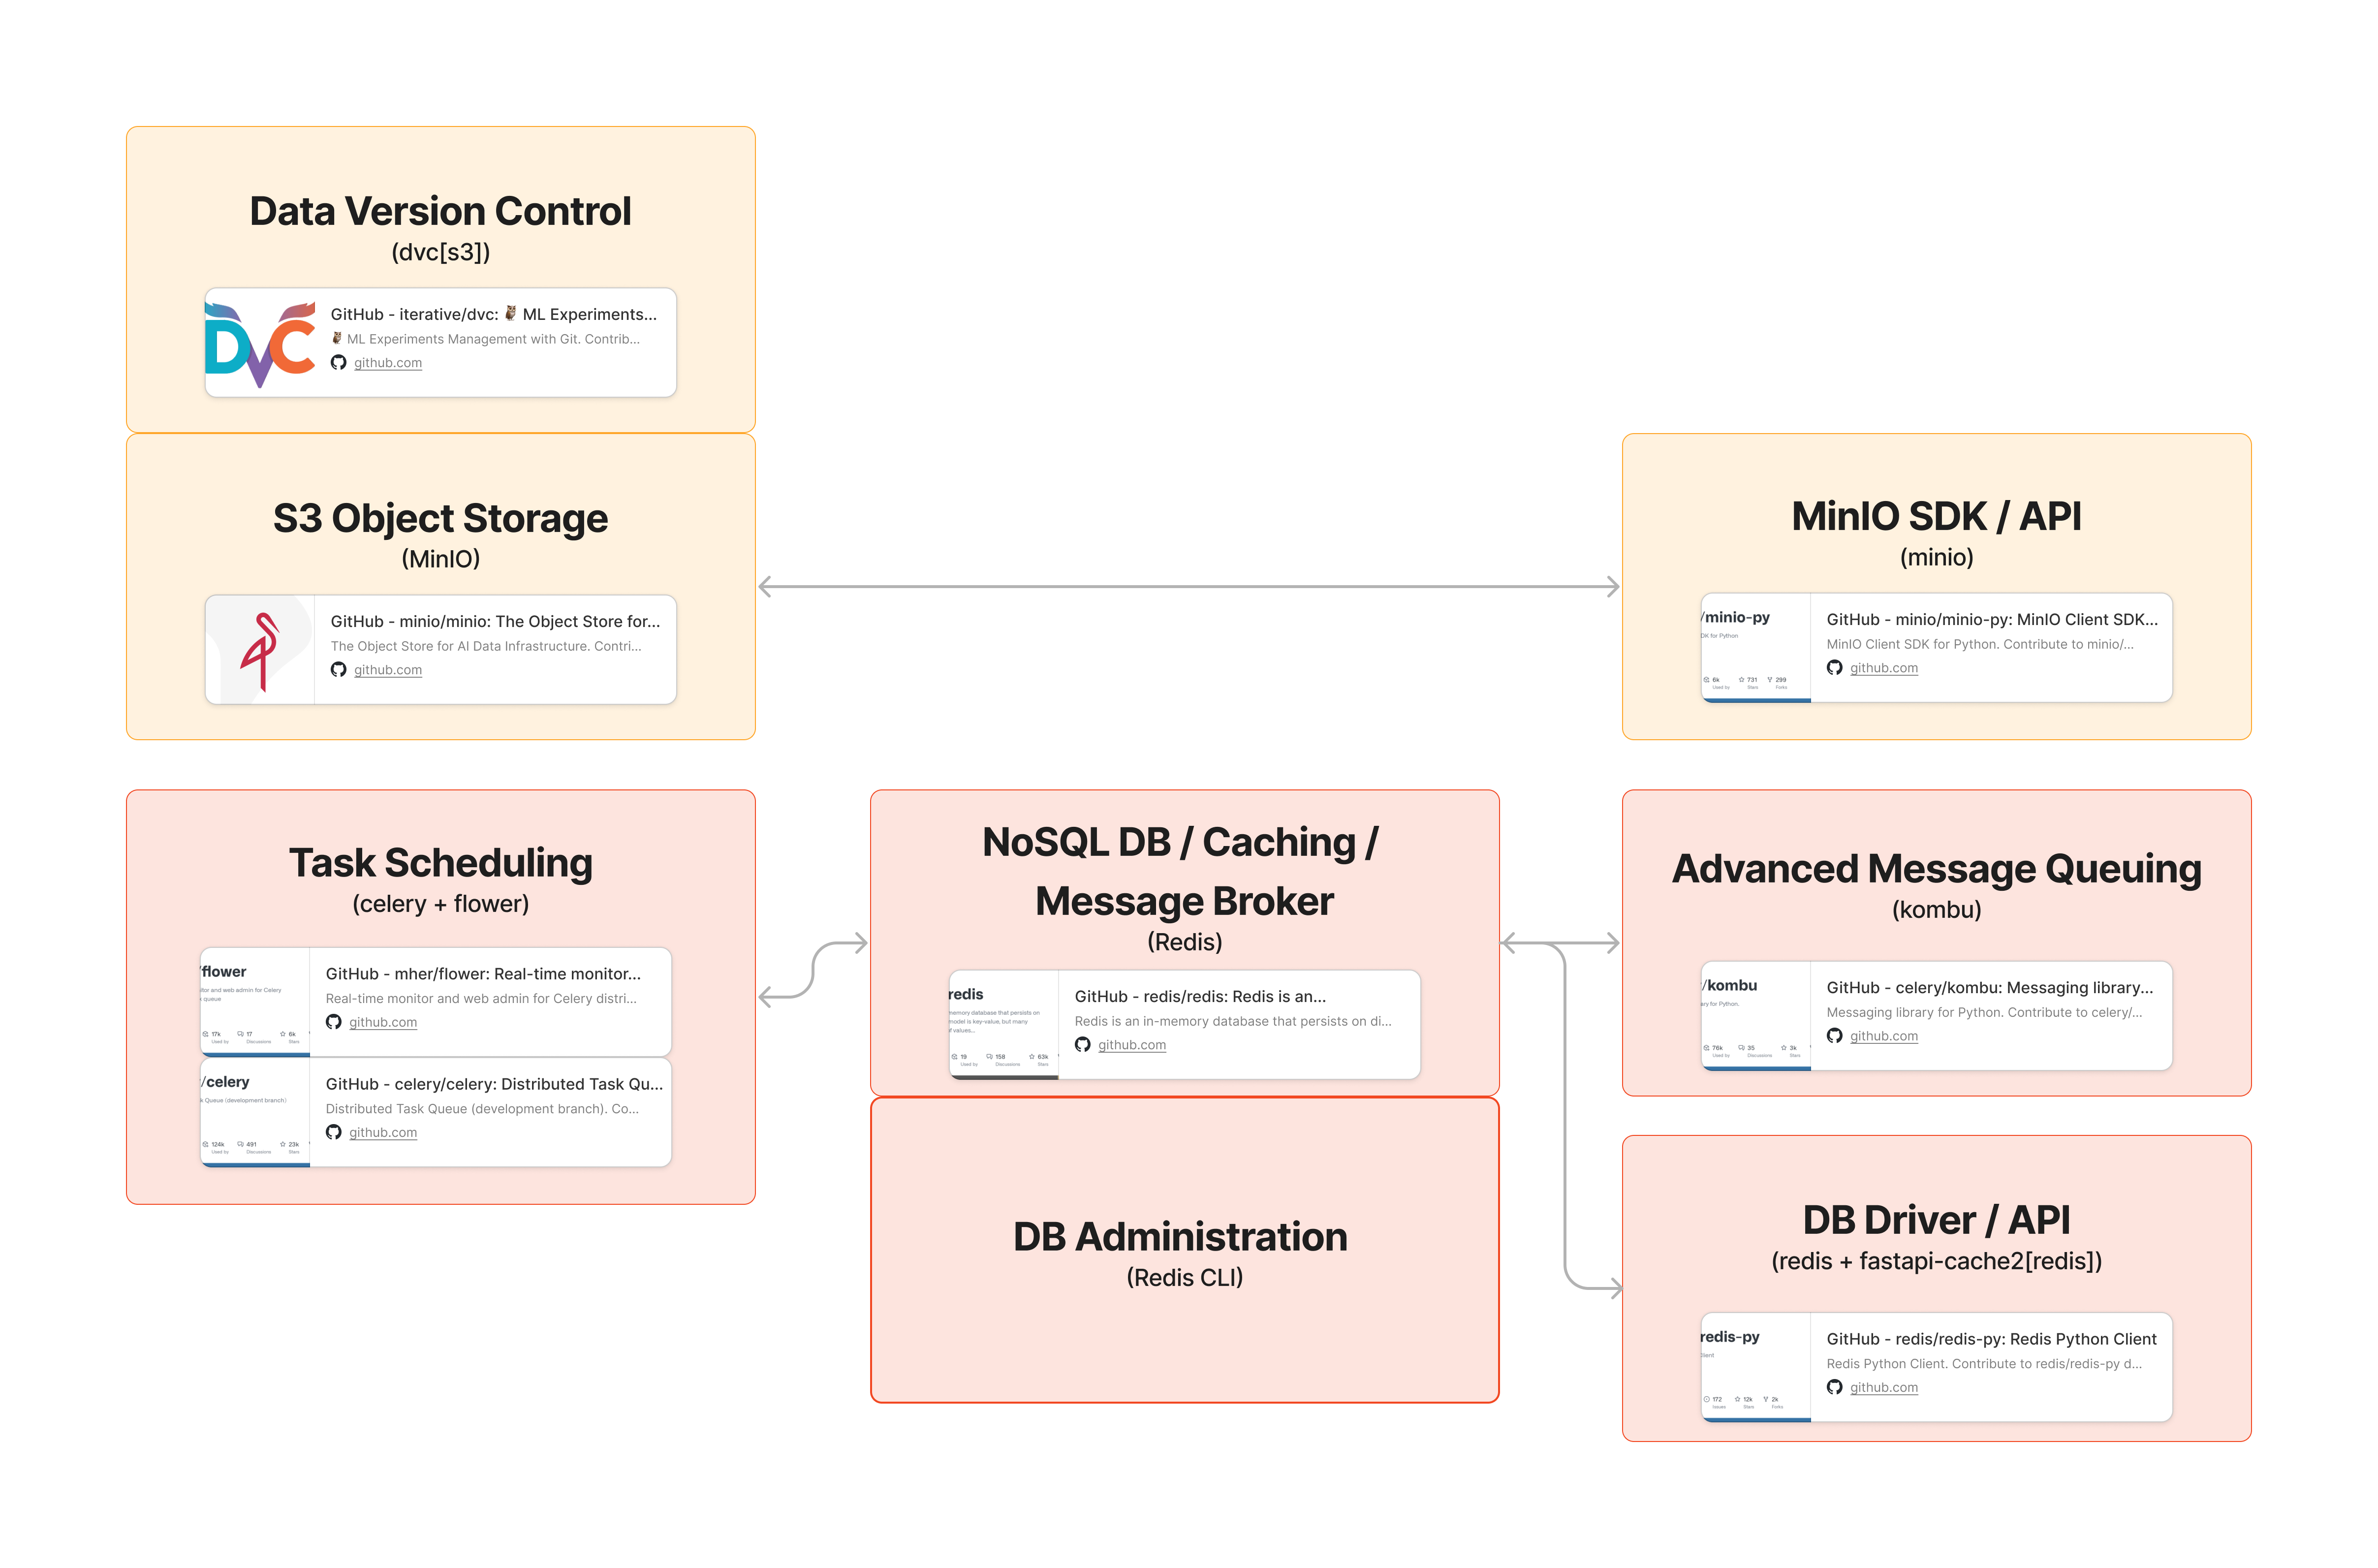
\includegraphics[width=1.0\textwidth]{figures/figure_2_31.png}
% \\
% \parbox[t]{\textwidth}{\vspace{1ex}\large\hspace*{7.5mm}}
\captionsetup{style=figureStyle}
\caption{Possible additional elements to the practical part of web scraping}\label{fig.2.31}
\end{figure}

- Project deployment should consider the deployment toolkit used by major companies, such as Kubernetes for containers orchestration, and automate processes with Ansible. However, these things require more server resources for the testing environment and subsequent practical experiments.
